\documentclass{report}
\usepackage[utf8]{inputenc}
\usepackage{amssymb}
\usepackage{amsmath}
\usepackage{hyperref}
\usepackage{tcolorbox}
\usepackage{bm}
\tcbuselibrary{theorems}
\usepackage{physics}
\usepackage{graphicx}



% Things I use, but too lazy to find how again

%%%%%%%%%%%%%%%%%%%%%%%%%%%%%%%%%%%%%%%%%%%%%%%%%%%%
% Make a hyperlink to another section:
% \hyperref[sec:hello]{Word of text} (set link to hello)

% \section{Hello World} 
% \label{sec:hello} (define a label for the section
%%%%%%%%%%%%%%%%%%%%%%%%%%%%%%%%%%%%%%%%%%%%%%%%%%%%
% Make an unordered list:
% \begin{itemize}
%   \item 
%   \item
% \end{itemize}
%%%%%%%%%%%%%%%%%%%%%%%%%%%%%%%%%%%%%%%%%%%%%%%%%%%%
% Make an ordered list:
% \begin{enumerate}
%   \item 
%   \item
% \end{itemize}
%%%%%%%%%%%%%%%%%%%%%%%%%%%%%%%%%%%%%%%%%%%%%%%%%%%%
% Make a matrix
%\begin{bmatrix}
%        x_1y_1 & x_1y_2 & \dots  & x_1y_m \\
%        x_2y_1 & x_2y_2 & \dots  & x_2y_m \\
%        \vdots & \vdots & \ddots & \vdots \\
%        x_ny_1 & a_{m2} & \dots  & x_ny_m \\
%   \end{bmatrix}
%%%%%%%%%%%%%%%%%%%%%%%%%%%%%%%%%%%%%%%%%%%%%%%%%%%%
% Make an equation:
% \begin{equation}
% ...
% \end{equation}
%%%%%%%%%%%%%%%%%%%%%%%%%%%%%%%%%%%%%%%%%%%%%%%%%%%%
% Theorems:
%\begin{mytheo}{Title}{NameOfTheorem}
% ...
%\end{mytheo}
%%%%%%%%%%%%%%%%%%%%%%%%%%%%%%%%%%%%%%%%%%%%%%%%%%%%

% N'th order linear equation
% $$y^{(n)}(t) + ... + p_1(t)y'(t) + p_0(t)y(t) = 0$$
%%%%%%%%%%%%%%%%%%%%%%%%%%%%%%%%%%%%%%%%%%%%%%%%%%%%

\newtcbtheorem[number within=section]{mytheo}{Theorem}
{colback=orange!5,colframe=red!35!black,fonttitle=\bfseries}{th}



\hypersetup{
    pdftitle={Differential Equations},
    pdfpagemode=FullScreen,
    linkbordercolor = {red},
}




\title{Differential Equations}
\author{Arun Khanna}
\date{}

\begin{document}

\maketitle
\tableofcontents

\chapter{First-order case}
\section{Types of Differential Equations}
Differential equations come in many types. This is a reference to look back into if you forget.
\section{Order of a differential equation}
The order of a differential equation is simply the highest derivative term in it, once it has been simplified as much as possible. For example:
$$y'' + 5y + 3 = 0$$
is a second order differential equation.

\section{}



\chapter{Existence of Solutions in Linear Differential Equations}
\section{Introduction}
Linear differential equations have interesting properties that allow us to solve them in convenient ways.

What does it mean to be linear anyway? For matrices, a linear transformation is simplify defined to be a transformation such that the even spacing of the grid-lines is preserved. However, generally, a function or transformation is defined to be linear if and only if it satisfies the following properties.

\begin{mytheo}{Linearity of a transformation}{lin}
    A transformation $T$ is defined to be linear if for inputs $\mathbf{v_1}$ and $\mathbf{v_2}$
    \begin{enumerate}
        \item $T(\mathbf{v_1}+\mathbf{v_2}) = T(\mathbf{v_1}) + T(\mathbf{v_2})$
        \item $T(c\mathbf{v_1}) = cT(\mathbf{v_1})$, where $c$ is a scalar constant
   \end{enumerate}
\end{mytheo}

A fascinating result of calculus is that derivatives are linear because they satisfy these two properties! Thus we can examine the linearity (or lack thereof) of differential equations, which are just equations connecting the various derivatives of the function together.

What does it mean to say that a differential equation is linear? It means that given two functions $y_1(t)$ and $y_2(t)$ satisfying the differential equation, that $y(t) = c_1y_1(t) + c_2y_2(t)$ should also satisfy the differential equation. It turns out that this condition is equivalent to having a differential equation in the form of:

\begin{mytheo}{Linearity of homogeneous differential equations}{lin_diff}
    A homogeneous differential equation is linear if and only if:
    $$y^{(n)}(t) + ... + p_1(t)y'(t) + p_0(t)y(t) = 0$$
\end{mytheo}


where all the coefficients of the derivatives of y are only functions of t and not y. For example, this would NOT be a linear differential equation:

$$y'' + 2yy' = 0$$
because of the $2y$ coefficient on $y'$.

What does having no coefficients dependent on y have anything to do with linearity? We know that all the derivative terms ($y^(n), ..., y'', y', y)$ must satisfy the definition of linearity because the derivative is a linear operator. However, if the coefficient is dependent on y in any way, adding two different potential solutions $y_1, y_2$ will NOT give us the same thing as adding up the individual solutions. We can see that in the example above:
$$(y_1+y_2)''+2(y_1+y_2)(y_1+y_2)'+3 = y_1'' + y_2'' + 2y_1y_1'+2y_1y_2' +2y_2y_1'+2y_2y_2'$$
$$=(y_1''+2y_1y_1')+ (y_2''+2y_2y_2')+2y_2y_1+2y_1y_2$$

Notice how taking $y = y_1+y_2$ and plugging it into the equation gives us the same thing as summing the individual results of plugging in $y_1$ and $y_2$, but with the additional garbage of $2y_2y_1+2y_1y_2$

\begin{mytheo}{Existence and Uniqueness Theorem}{Ex&Un}
    Given an n'th order linear differential equation
    $$y^{(n)}(t) + ... + p_1(t)y'(t) + p_0(t)y(t) = g(t)$$
    and n initial conditions at a time period $t_0$ inan interval $I$ where $p_{n-1}(t)$, $\dots$, $p_1(t)$, and $p_0(t)$ is continuous
    
    $y(t_0) = a_0$, $y'(t_0) = a_1$, \dots, $y^{(n)}(t_0) = a_n$
    
    there exists only one unique solution $y(t) = \phi(t)$ over the interval I.
    
\end{mytheo}


\section{Principle of Superposition}

\begin{mytheo}{Principle of Superposition}{super}
 If we have a homogeneous linear differential equation of the form:
 $$y^{(n)}(t) + ... + p_1(t)y'(t) + p_0(t)y(t) = 0$$
 and n solutions, $y_1(t)$, $y_2(t)$, $\dots$, $y_n(t)$, then any linear combination $c_1y_1(t) + c_2y_2(t) + \dots + c_ny_n(t)$ is also a solution.
\end{mytheo}


Why?
Well, a homogeneous equation of degree $m$ is in the form:
$$L[y] = y^{(n)}(t) + ... + p(t)y'(t) + q(t)y(t) = 0$$
We know that since this is linear, $L[y_i+y_j] = L[y_i] + L[y_j]$ and $L[cy_i] = cL[y_i]$ for a constant $c$.

If $y_1, ..., y_n$ are solutions, they must all satisfy $L[y_i] = 0$. Thus,
$$L[c_1y_1+c_2y_2+...+c_ny_n] = c_1L[y_1] + c_2L[y_2] + ... + c_nL[y_n] = 0 + 0 + ... + 0 = 0$$
Thus, the linear combination satisfies the condition to be a solution for this differential equation.



\section{Unique Homogeneous Solution and the Wronskian}
In this section, we will consider second order homogeneous equations for simplicity, however, the results apply in general.

By \hyperref[th:Ex&Un]{The Existence and Uniqueness Theorem}, we know that for an n'th order linear homogeneous differential equation with n initial conditions that there exists one unique solution. How do we go about finding this one unique solution?

Say that we've found two solutions $y_1(t)$ and $y_2(t)$ to the differential equation:

$$y'' + p_1(t)y' + p_0(t)y = 0$$

$$\text{with } y(t_0) = a_0 \text{ and } y'(t_0) = a_1$$

By \hyperref[th:super]{superposition}, we know that any linear combination of $y_1(t)$ and $y_2(t)$ is a solution.
$$y(t) = c_1y_1(t) + c_2y_2(t)$$
By our initial conditions:
$$y(t_0) = c_1y_1(t_0) + c_2y_2(t_0) = a_0$$
$$y'(t_0) = c_1y'_1(t_0) + c_2y'_2(t_0) = a_1$$

Since the \hyperref[th:Ex&Un]{The Existence and Uniqueness Theorem} tells us there is only one solution satisfying the initial constraints, we should be able to get unique values for the coefficients of the equation $c_1$ and $c_2$. Representing the series of equations in matrix form:
$$
\begin{bmatrix}
    y_1(t_0) & y_2(t_0) \\
    y_1'(t_0) & y_2'(t_0) \\
\end{bmatrix}
\begin{bmatrix}
    c_1 \\
    c_2 \\
\end{bmatrix}
=
\begin{bmatrix}
    a_0 \\
    a_1 \\
\end{bmatrix}
$$

The only way we are able to get values for $c_1$ and $c_2$ that satisfy this equation is if the matrix 
$\begin{bmatrix}
    y_1(t_0) & y_2(t_0) \\
    y_1'(t_0) & y_2'(t_0) \\
\end{bmatrix}$,
also known as the \textbf{Fundamental Matrix} is invertible. An equivalent condition to invertibilitity of a matrix is that its determinant is non-zero(columns are linearly independent). Thus provided that

$$\text{det}\left(\begin{bmatrix}
    y_1(t_0) & y_2(t_0) \\
    y_1'(t_0) & y_2'(t_0) \\
\end{bmatrix}\right)
\neq 0
$$
we can always find a solution for the coefficients $c_1$ and $c_2$
$$
\begin{bmatrix}
    c_1 \\
    c_2 \\
\end{bmatrix}
=
\begin{bmatrix}
    y_1(t_0) & y_2(t_0) \\
    y_1'(t_0) & y_2'(t_0) \\
\end{bmatrix}^{-1}
\begin{bmatrix}
    a_0 \\
    a_1 \\
\end{bmatrix}
$$

The determinant of the fundamental matrix is called the \textbf{Wronskian} and has a number of interesting properties. 

Thus, we can conclude that in general:

\begin{mytheo}{Unique Homogeneous Solution}{unHomSol}
 Given a homogeneous equation of the form:
  $$y^{(n)}(t) + ... + p_1(t)y'(t) + p_0(t)y(t) = 0$$
  and $n$ solutions $y_1(t)$, $y_2(t)$, $\dots$, $y_n(t)$ such that there exists a $t_0$ where the determinant of the fundamental matrix (the Wronskian) is non-zero:
  $$\text{det}\left(\begin{bmatrix}
    y_1(t_0) & y_2(t_0) & \dots  & y_n(t_0) \\
    y_1'(t_0) & y_2'(t_0) & \dots  & y_n'(t_0) \\
    \vdots & \vdots & \ddots & \vdots \\
    y_1^{(n)}(t_0) & y_2^{(n)}(t_0) & \dots  & y_n^{(n)}(t_0) \\
    \end{bmatrix}\right)
    \neq 0
    $$
 The general unique solution to the differential equation is in the form of:
 $$\phi(t) = c_1y_1(t) + c_2y_2(t) + \dots + c_ny_n(t)$$
 where $c_1, \dots, c_n$ can be determined given $n$ conditions of the form:
 $y(t_0) = a_0$, $y'(t_0) = a_1$, $\dots$, $y^{(n-1)}(t_0) = a_n$ by 
 $$
\begin{bmatrix}
    c_1 \\
    c_2 \\
    \vdots \\
    c_n
\end{bmatrix}
=
\begin{bmatrix}
    y_1(t_0) & y_2(t_0) & \dots  & y_n(t_0) \\
    y_1'(t_0) & y_2'(t_0) & \dots  & y_n'(t_0) \\
    \vdots & \vdots & \ddots & \vdots \\
    y_1^{(n)}(t_0) & y_2^{(n)}(t_0) & \dots  & y_n^{(n)}(t_0) \\
    \end{bmatrix}^{-1}
\begin{bmatrix}
    a_0 \\
    a_1 \\
    \vdots \\ 
    a_n
\end{bmatrix}
$$
\end{mytheo}

\section{Linear Independence and the Wronskian}
\section{Linear Dependence}
What does it mean for a function to be \textbf{linearly dependent} on another function? 

Recall what linear dependence means for vectors. When we have two vectors that are linearly dependant, we can represent one vector as a scaled version of the other:

[Insert Picture]

Algebraically, for two vectors $\bm{\vec{v_1}}$ and $\bm{\vec{v_2}}$ are \textbf{linearly independent} when:
$$\bm{\vec{v_1}} = c\bm{\vec{v_2}}$$
for some constant $c$

\textbf{Linear dependence} between two vectors occurs when this is not true, it is impossible to recreate one of the two linearly dependent vectors by just scaling the other one:

[Insert Picture]

Algebraically, for two vectors $\bm{\vec{v_1}}$ and $\bm{\vec{v_2}}$ are \textbf{linearly independent} when:
$$\bm{\vec{v_1}} \neq c\bm{\vec{v_2}}$$
for any constant $c$

When dealing with functions, the definitions of linearly dependence and independence are really similar:

\begin{mytheo}{Linear Dependence and Independence of functions}{lin_func}
    Two functions $f(t)$ and $g(t)$ are \textbf{linearly independent} on an interval $I$ if and only if for every $t$ in $I$, the result of one function can be represented as a scalar multiple of the other function:
    $$\bm{f(t)} = c\bm{g(t)} \text{ for all $t \in I$}$$
    This is equivalent to saying (as most textbooks present it):
    $$c_1\bm{f(t)} + c_2\bm{g(t)} = 0 \text{ for all $t \in I$}$$
    for non-zero constants $c_1$ and $c_2$
    
    Similarly, \textbf{linear dependence} is defined as when these conditions are not met, i.e.:
    $$\bm{f(t_0)} \neq c\bm{g(t)} \text{ for a $t_0 \in I$}$$
    or:
    $$c_1\bm{f(t_0)} + c_2\bm{g(t_0)} = 0 \text{ for a $t_0 \in I$}$$
    for only constants $c_1$ and $c_2$ equal to 0
    
\end{mytheo}

These definitions apply similarly in higher dimensions, linear independence of $n$ functions is the same thing as all of the $n$ functions being linearly independent to one another.

\section{Wronskian and Linear Independence}
How does the Wronskian relate to linear independence of functions?

Fascinatingly, finding the Wronskian of any two functions can tell us directly if the two functions are linearly independent:

\begin{mytheo}{Wronskian and linear independence}{wronLinInd}
    Consider two functions $f(t)$ and $g(t)$ defined as continuous on some interval $I$. If the Wronskian of these two functions is non-zero for a $t_0$ in the interval $I$, then the two functions are \textbf{linearly independence}. 
    
    $$W(f(t),g(t))(t_0) = \text{det}\left(\begin{bmatrix}
    f(t_0) & g(t_0) \\
    f'(t_0) & g'(t_0) \\
    \end{bmatrix}\right)
    \neq 0 $$
    $$\implies c_1\bm{f(t_0)} + c_2\bm{g(t_0)} = 0$$ 
    for a $t_0 \in I$ only for constants $c_1=c_2=0$ (linear independence).
\end{mytheo}
  
\hyperref[sec:prWronLinInd]{The proof can be found in the appendix}


Note that the implication is in only one way. This is important!! In general, if the Wronskian is zero for all $t \in I$, that does \textbf{not} necessarily mean that functions are linearly dependant. 
    
An example of this occurring are the functions $f(t) = t^3$ and $g(t) = |t|t^2$ over the interval $-\infty < t < \infty$. These functions are linearly independent over the interval, but the Wronskian is in fact 0 everywhere!!
\\ \\
By using basic logic principles, the contrapositive of a true implication is also true. Therefore, linearly dependent functions have a Wronskian zero everywhere in the interval in which they are defined to be linearly dependant:
    
\begin{mytheo}{Linear dependence and the Wronskian}{wronLinDep}
    Consider two functions $f(t)$ and $g(t)$ defined as continuous on some interval $I$. If the functions are \textbf{linearly dependent} for all $t \in I$, then the Wronskian is zero everywhere.
    
    $$c_1\bm{f(t)} + c_2\bm{g(t)} = 0$$ 
    for non-zero constants $c_1$ and $c_2$ (linear dependence)
    
    $$ \implies W(f(t),g(t))(t) = \text{det}\left(\begin{bmatrix}
    f(t) & g(t) \\
    f'(t) & g'(t) \\
    \end{bmatrix}\right)
    = 0 \text{, for all $t \in I$}$$
\end{mytheo}


\section{Abel's Theorem}
Let's go back to the case of second order homogeneous linear differential equations. Say we have the equation:
$$y''(t) + p_1(t)y'(t) + p_0(t)y(t) = 0$$
For any two solutions $y_1(t)$ and $y_2(t)$ which may be fundamental solutions or not, Abel's theorem yields an extremely powerful result:

\begin{mytheo}{Abel's Theorem}{abel_thm}
    Say we have a second order homogeneous linear differential equation of the form 
    $$y''(t) + p_1(t)y'(t) + p_0(t)y(t) = 0$$
    over an interval $I$ where the coefficients are continuous and the first and second derivatives of $y(t)$ are continuous and defined.
    In addition, say we have two solutions $y_1(t)$ and $y_2(t)$ that satisfy these constraints.
    
    According to Abel's theorem, the Wronskian of any two solutions will precisely be:
    
    $$W(y_1(t), y_2(t))(t) = \text{det}\left(\begin{bmatrix}
    y_1(t) & y_2(t) \\
    y_1'(t) & y_2'(t) \\
    \end{bmatrix}\right)$$
    $$= c(y_1(t),y_2(t))\exp{\left[-\int{p_1(t)dt}\right]}$$
    where $c$ is a constant that depends on $y_1(t)$ and $y_2(t)$ but not $t$.
\end{mytheo}

\hyperref[sec:abel]{The proof can be found in the appendix.}
\newline


This theorem tells us that the Wronskian of any two solutions to a second-order linear homogeneous differential equation differ only by a constant multiple.


One consequence of Abel's theorem is that if the Wronskian is non-zero at one point in the interval $I$, it is non-zero everywhere. Similarly, if the Wronskian is zero at one point, it is zero everywhere. This is because $c$ determines whether or not the Wronskian will be zero or non-zero at a point $t_0 \in I$ since the exponential term will always be non-zero. Since $c$ is universally defined in the interval (not dependent on $t$), it will be 0 or non-zero. 

This leads us to another important result:

\begin{mytheo}{Wronskian for two solutions}{wron_two_sol}
    The Wronskian for any two solutions of a second order linear homogeneous differential equation defined on some interval $I$ is either 0 everywhere on this interval or always non-zero.
    $$
    W(y_1(t), y_2(t))(t) = \text{det}\left(\begin{bmatrix}
    y_1(t) & y_2(t) \\
    y_1'(t) & y_2'(t) \\
    \end{bmatrix}\right) = 0
    $$
    for all $t \in I$
    
    OR
    
    $$
    W(y_1(t), y_2(t))(t) = \text{det}\left(\begin{bmatrix}
    y_1(t) & y_2(t) \\
    y_1'(t) & y_2'(t) \\
    \end{bmatrix}\right) \neq 0
    $$
    for all $t \in I$
\end{mytheo}

This falls directly from Abel's theorem (the constant is either 0 or non-zero on the interval $I$). 

This means that if we find the Wronskian to be 0 at any point $t_0$ in the interval, the Wronskian will be 0 everywhere on the interval. Similarly, if it is non-zero at any point, it will be non-zero everywhere. 

This is a powerful fact! This will be made even more powerful in the next section:

\section{Fundamental Solutions and Linear Dependence}
We know two major things from the previous sections about the Wronskian of two solutions to a homogeneous linear differential equation:
\begin{enumerate}
    \item \hyperref[th:unHomSol]{$W(y_1(t), y_2(t))(t_0)\neq 0 \implies $ $y_1(t)$ and $y_2(t)$ span the solution space}
    \item \hyperref[th:wronLinInd]{$W(y_1(t), y_2(t))(t_0)\neq 0 \implies $ $y_1(t)$ and $y_2(t)$ are linearly independent}
\end{enumerate}

A question that may be asked is whether linear independence and spanning the solution space of two solutions can be connected. This would be a beautiful connection to linear algebra and differential equations, where having linearly independent vectors spans the space we're considering. In fact, there is a connection through the Wronskian:


\begin{mytheo}{Wronskian and Linear Dep of solutions}{WrLinDep}
    Say we have a second order homogeneous linear differential equation of the form 
    $$y''(t) + p_1(t)y'(t) + p_0(t)y(t) = 0$$
    over an interval $I$ where the coefficients are continuous and the first and second derivatives of $y(t)$ are continuous and defined. 
    In addition say we have found two solutions $y_1(t)$ and $y_2(t)$ for this differential equation.
    
    The Wronskian of $y_1(t)$ and $y_2(t)$ will only be 0 if and only if $y_1(t)$ and $y_2(t)$ are Linearly Dependent. 
    
    In other words:
    
    $$W(y_1(t), y_2(t))(t) = 0 \implies \text{Linear Dependence}$$
    
    $$ \text{Linear Dependence} \implies W(y_1(t), y_2(t))(t) = 0$$
    
\end{mytheo}


\hyperref[sec:PrWrLinDep]{The proof of this can be found in the appendix.}

The converse is also directly implied:

\begin{mytheo}{Wronskian and Linear Ind of solutions}{WrLinIn}
    Say we have a second order homogeneous linear differential equation of the form 
    $$y''(t) + p_1(t)y'(t) + p_0(t)y(t) = 0$$
    over an interval $I$ where the coefficients are continuous and the first and second derivatives of $y(t)$ are continuous and defined. 
    In addition say we have found two solutions $y_1(t)$ and $y_2(t)$ for this differential equation.
    
    The Wronskian of $y_1(t)$ and $y_2(t)$ will only be non-zero if and only if $y_1(t)$ and $y_2(t)$ are Linearly Independent. 
    
    In other words:
    
    $$W(y_1(t), y_2(t))(t_0) \neq 0 \implies \text{Linear Independence}$$
    
   $$ \text{Linear Independence} \implies W(y_1(t), y_2(t))(t_0) \neq 0$$
    
\end{mytheo}


Since the Wronskian being non-zero at some point is equivalent to linear independence for two solutions to a linear homogeneous second-order differential equation:

\begin{mytheo}{Fundamental solutions and Linear Ind}{fund_sol}
    If two solutions to a linear homogeneous second-order differential equation $y_1(t)$ and $y_2(t)$ are linearly independent, they span the solution space for the differential equation.
\end{mytheo}

Thus, all of these facts are equivalent:

\begin{mytheo}{Equivalencies for linearly independent solutions}{EqLinInd}
    For two solutions $y_1(t)$ and $y_2(t)$ on some interval $I$ of the linear homogeneous second-order differential equation:
    $$y''(t) + p_1(t)y'(t) + p_0(t)y(t) = 0$$
    all of the following are equivalent:
    \begin{enumerate}
        \item The Wronskian of the solutions is non-zero at some point $t_0 \in I$ 
        $$W(y_1(t), y_2(t))(t_0) \neq 0 $$
        \item The Wronskian of the solutions is non-zero at \textbf{all points} $t \in I$ 
        $$W(y_1(t), y_2(t))(t) \neq 0 $$
        \item The two solutions are linearly independent:
        $$c_1y_1(t_0) + c_2y_2(t_0) = 0$$
        is only satisfied for $c_1=c_2=0$ at some $t_0 \in I$
        \item The two solutions span the entire solution space for the differential equation:
        $$\phi(t) = c_1y_1(t) + c_2y_2(t)$$
        satisfies the differential equation for all $t \in I$
    
    \end{enumerate}
    
\end{mytheo}


Similarly, the opposite is true:

\begin{mytheo}{Equivalencies for linearly dependent solutions}{EqLinDep}
    For two solutions $y_1(t)$ and $y_2(t)$ on some interval $I$ of the linear homogeneous second-order differential equation:
    $$y''(t) + p_1(t)y'(t) + p_0(t)y(t) = 0$$
    all of the following are equivalent:
    \begin{enumerate}
        \item The Wronskian of the solutions is zero at some point $t_0 \in I$ 
        $$W(y_1(t), y_2(t))(t_0) = 0 $$
        \item The Wronskian of the solutions is zero at \textbf{all points} $t \in I$ 
        $$W(y_1(t), y_2(t))(t) = 0 $$
        \item The two solutions are linearly dependent:
        $$c_1y_1(t) + c_2y_2(t) = 0$$
        is only satisfied for some non-zero $c_1$ and $c_2$ for all $t \in I$
        \item The two solutions \textbf{do not} span the entire solution space for the differential equation:
        $$\phi(t) = c_1y_1(t) + c_2y_2(t)$$
        \textbf{does not} satisfy the differential equation for all $t \in I$
    
    \end{enumerate}
    
\end{mytheo}





\chapter{Linear Differential Equation with Constant Coefficients}
\section{Introduction}

Let's zoom into the specific case of linear homogeneous differential equations with constant coefficients:

That is a differential equation in the form of:
$$y^{(n)}(t) + ... + a_1y'(t) + a_0y(t) = 0$$

In this section we will mostly consider second order differential equations, since they are significantly easier to solve, however, the results apply in general for any $n^th$ degree polynomial.

So let us look at that case:
$$y''(t) + a_1y'(t) + a_0y$$

What happens if we try a solution in the form of $y(t) = Ce^{rt}$?

When we plug it into our equation and simplify, we get (by the property of taking derivatives of exponents):

$$(Ce^{rt})'' + a_1(Ce^{rt})' + a_0Ce^{rt} = 0$$
$$(r^2cCe^{rt}+a_1rCe^{rt}+a_0Ce^{rt} = 0$$
Taking out $Ce^{rt}$, 
$$(r^2+a_1r+a_0)e^{rt} = 0$$

Since, $e^{rt}$ is always greater than 0, we can divide by both sides to get an expression for $r$:

$$r^2+a_1r+a_0 = 0$$

To recap, for the differential equation above $y(t) = Ce^{rt}$ is a solution for any $r$ that satisfies the polynomial equation above!

This holds in general:

\begin{mytheo}{A Constant Coefficients Solution}{constSol}
    For an n'th order differential equation with constant coefficients in the form:
    $$y^{(n)}(t) + ... + a_1y'(t) + a_0y(t) = 0$$
    
    $y(t) = Ce^{rt}$ will be a solution as long as it satisfies the following polynomial equation:
    
    $$r^n+\dots+a_1r+a_0=0$$
    
    The polynomial is called the \textbf{characteristic polynomial} of the differential equation above.
\end{mytheo}
The proof can be found in the appendix.

From the chapter above, we showed that in order for us to have the complete solution a linear differential equation of $n$'th degree, we need $n$ linearly independent solutions. Since $y(t) = Ce^{rt}$ is always a solution to the differential equation, it will help us find the fundamental solution. 
In the sections below, we will consider finding the complete solution to the linear differential equation with constant coefficients in the following cases for the roots of the characteristic polynomial:
\begin{enumerate}
    \item Roots are real and unique
    \item Roots are complex
    \item Some Roots are repeated
\end{enumerate}


\section{Real Unique Roots}

The following theorem is important:

\begin{mytheo}{Linear Independence of Exponentials of Different Degrees}{expLinInd}
    Consider two functions $y_1(t) = e^{r_1t}$ and $y_2(t) = e^{r_2t}$ such that $r_1 \neq r_2$. 
    \\
    \\
    The functions $y_1(t) = e^{r_1t}$ and $y_2(t) = e^{r_2t}$ has a Wronskian that is always non-zero and are linearly independent.
\end{mytheo}

\hyperref[sec:prExpLinInd]{The proof is in the appendix.}

If we have the differential equation, 
$$y^{(n)}(t) + ... + a_1y'(t) + a_0y(t) = 0$$
and the following characteristic polynomial equation:

$$r^n+\dots+a_1r+a_0=0$$

Say that we solve this polynomial equation and get $n$ real unique roots such that $r_1 \neq r_2 \neq \dots r_n$. 

Then we know that $y_1(t) = Ce^{r_1t}, y_2(t) = Ce^{r_2t}, \dots y_n(t)Ce^{r_nt}$ are all \hyperref[th:constSol]{solutions to the differential equation}. We also know that all of these solutions are \hyperref[th:expLinInd]{linearly independent since $r_1 \neq r_2 \neq \dots r_n$}. Because of these facts, we know that the following function:
$$\phi(t) = c_1e^{r_1t}+c_2e^{r_2t}+\dots c_ne^{r_nt}$$

must be the \hyperref[th:EqLinInd]{fundamental solution the differential equation since it is the combination of $n$ linearly independent solutions for a $n$'th order linear differential equation.}

Thus:

\begin{mytheo}{Complete Solution to Linear Differential Equation with Real Unique Roots}{compSolReUn}
    For a linear differential equation with constant coefficients in the form:
    $$y^{(n)}(t) + ... + a_1y'(t) + a_0y(t) = 0$$
    If we solve the characteristic polynomial:
    $$r^n+\dots+a_1r+a_0=0$$
    and get $n$ real unique roots $r_1 \neq r_2 \neq \dots r_n$, the fundamental solution is:
    
    $$\phi(t) = c_1e^{r_1t}+c_2e^{r_2t}+\dots c_ne^{r_nt}$$

\end{mytheo}


\section{Complex Roots}
\label{sec:comRoot}
If we have a polynomial of the form:
$$y^{(n)}(t) + ... + a_1y'(t) + a_0y(t) = 0$$
and instead of getting unique real roots, we get complex roots of the form $a+bi$, we could proceed as we did before and have solutions:
$$e^{(a_1+b_1i)t}, e^{(a_2+b_2i)t}, \dots, e^{(a_n+b_ni)t}$$

This would in fact be valid. However, there is a way we can take this equation and turn it into a form that is significantly easier to both visualize and easier to apply to actual physical solutions.

First, we need to introduce Euler's formula:

\begin{mytheo}{Euler's Formula}{euler}
    We can express the exponential of an imaginary number with sines and cosines using Euler's formula.
    
    $$e^{bit} = \cos(bt) + i\sin(bt)$$
\end{mytheo}

Another important theorem in algebra is the complex conjugate root theorem:

\begin{mytheo}{Complex Conjugate Root Theorem}{comConjRoot}
    For any $n$'th degree polynomial in the form:
    $$r^n+\dots+a_1r+a_0=0$$
    If the complex number $r_1=a+bi$ is a root, then another root has to be $r_2 = a-bi$. 
    In other words, if one complex number is a root of a polynomial, then it is neccessarily the case that the complex conjugate of that root is another root (complex conjugates always come in pairs).
\end{mytheo}

Both of these theorems hold true in general and are given without proof.

By the \hyperref[th:comConjRoot]{Complex Conjugate theorem}, if $r_1=a+bi$ is a solution to the characteristic polynomial $r_2 = a-bi$ must also be a solution.

Thus when $y_1(t) = e^{(a+bi)t}$ is a solution to a linear homogeneous differential equation with constant coefficients, $y_2(t) = e^{(a-bi)t}$ also must be (since they both solve the same characteristic polynomial).

Because of \hyperref[th:euler]{Euler's formula} we can represent these solutions as:
$$y_1(t) = e^{at}(\cos{bt}+i\sin{bt}$$
$$y_2(t) = e^{at}(\cos{bt}-i\sin{bt}$$

Because of superposition $y_3(t) =\frac{1}{2}y_1(t)+\frac{1}{2}y_2(t)$ is also a solution:

$$y_3(t) = \frac{1}{2}e^{at}(\cos{bt}+i\sin{bt})+ \frac{1}{2}e^{at}(\cos{bt}-i\sin{bt})$$
$$=e^{at}(\frac{1}{2}\cos{bt} + \frac{1}{2}\cos{bt})$$
$$=e^{at}\cos{bt}$$

Similarly, $y_4(t)=-\frac{1}{2}iy_1(t) + \frac{1}{2}iy_2(t)$ is also a solution:
$$y_4(t) = -\frac{1}{2}ie^{at}(\cos{bt}+i\sin{bt})  \frac{1}{2}e^{at}(\cos{bt}-i\sin{bt})$$
$$ie^{at}(-\frac{1}{2}i\sin{bt} - \frac{1}{2}i\sin{bt})$$
$$-e^{at}(i^2\sin{bt})$$
$$e^{at}(\sin{bt})$$


\label{sinLin}
These two solutions formed by taking linear combinations of the complex solutions are real and furthermore they are \hyperref[sec:prSinLin]{linearly independent!}

Thus,

\begin{mytheo}{Real Solutions from Complex roots}{realFromComplex}
    If we have a differential equation in the form 
    $$y^{(n)}(t) + ... + a_1y'(t) + a_0y(t) = 0$$
    with the characteristic polynomial:
    $$r^n+\dots+a_1r+a_0=0$$
    if we solve this polynomial and get a complex pair of conjugate roots $r_1 = a+bi$ and $r_2 = a-bi$, we can represent two \textbf{real} solutions for the original differential equation as:
    $$y_1(t) = e^{at}(\cos{bt})$$
    $$y_2(t) = e^{at}(\sin{bt})$$
\end{mytheo}

\section{Repeated Roots}
What happens when we solve our characteristic equation and get a repeated root, i.e. $r_1=r_2$ solves our equation. Then we no longer have the $n$ linearly independent solutions we need to span our solution space anywhere.

The proof of the following theorem is long, but definitely worth looking at:


\begin{mytheo}{Linearly Independent Solutions with Repeated Roots}{linIndRep}
    If we have a differential equation in the form 
    $$y^{(n)}(t) + ... + a_1y'(t) + a_0y(t) = 0$$
    with the characteristic polynomial:
    $$r^n+\dots+a_1r+a_0=0$$
    If we solve this equation and end up getting two roots $r_i=r_j$ such that there are less than $n$ equations of the form $y(t) = e^{rt}$. 
    If $r_i$ is a repeated once in the characteristic solution, then we can find two linearly independent solutions:
    $$y_i(t) = e^{r_it}$$
    $$y_j(t) = te^{r_it}$$
    
    This applies in general. If $r_i$ is repeated $n$ times, all of the following are linearly independent solutions:
    $$y_1(t) = e^{r_it}$$
    $$y_2(t) = te^{r_it}$$
    $$\vdots$$
    $$y_n(t) = t^ne^{r_it}$$
\end{mytheo}

\label{repRoot}
\hyperref[sec:PrRepRoot]{The "proof" is presented in the appendix} for the specific case of second-order differential equation. 

Note that this means that for any homogeneous differential equation with constant coefficients, we can \textbf{always} find the solutions quite easily if we know the roots of the polynomial. Finding the roots, however may end up being very difficult (especially since there is no general formula for polynomials of degree 5 and above).


\section{Application: Spring-Mass System and Damping}
\subsection{Simple Harmonic Motion}
Consider a physics example of a mass attached to a theoretically mass-less spring with a spring-constant of $k$.

[insert picture]

When we pull the spring to the right by a small $\delta x$, by Hooke's law, the restoring force to its original force is proportial to the distance stretched. The direction is in the opposite direction of stretching. Thus,
$$F = -kx$$
This is equivalent to (by Newton's 2nd Law):
$$m\dv[2]{x}{t} = -kx$$
Further simplify we get:
$$\dv[2]{x}{t} + \frac{k}{m}x = 0$$

which is a second order differential equation with constant coefficients. We can solve this by finding the roots of the characteristic polynomial:

$$r^2+\frac{k}{m} = 0$$
$$r = 0 \pm \sqrt{-\frac{k}{m}}$$

Thus we have a complex root. We know from \hyperref[sec:comRoot]{the section above} that two solutions to this are:

$$y_1(t) = e^0\cos(\sqrt{\frac{k}{m}}t) = \cos(\sqrt{\frac{k}{m}}t)$$
$$y_2(t) = e^0\sin(\sqrt{\frac{k}{m}}t) = \sin(\sqrt{\frac{k}{m}}t)$$

and that in fact any linear combination of these two solutions will also be a solution.

$$y(t) = c_1\cos(\sqrt{\frac{k}{m}}t) + c_2\sin(\sqrt{\frac{k}{m}}t)$$

The following theorem can help simplify this even more:

\begin{mytheo}{Adding sines and cosines of same frequency}{sinPlusCosin}
    The linear combination of a sine and cosine function of the same frequency is itself a cosine function with a phase shift $\phi$:
    $$a\cos(\omega t) + b\sin(\omega t) = A\cos(\omega t - \phi)$$
    where $$A = \sqrt{a^2+b^2}$$ and $$\phi = \tan^{-1}(b/a)$$
\end{mytheo}
\hyperref[sec:prSinPlusCosin]{Two proofs are given in the appendix.}

Thus, an equivalent form is:
$$y(t) = A\cos(\sqrt{\frac{k}{m}} t - \phi)$$

In both representations of the solution, the constants can be determined by the initial conditions ($c_1, c_2$ in the first case and $A, \phi$ in the second).

Thus, the solution look something like this:

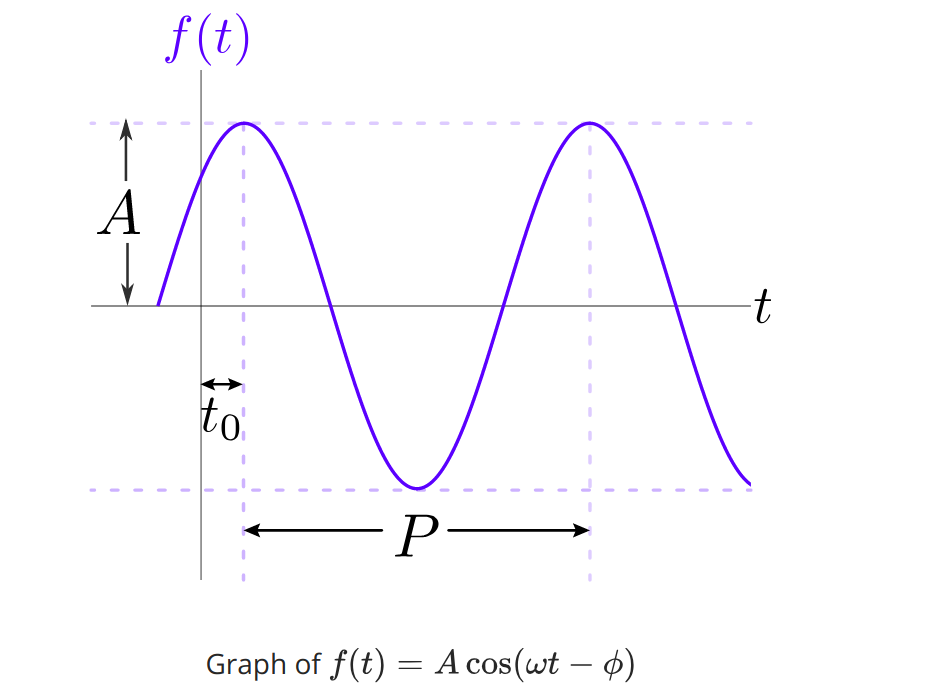
\includegraphics[scale=0.4]{cos_phase.png}


\subsection{Damping}

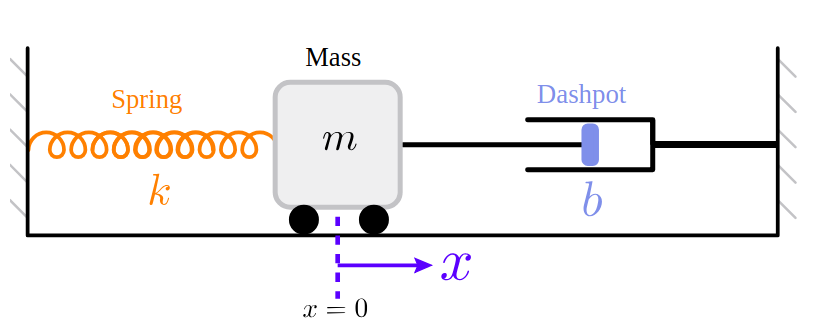
\includegraphics[scale=0.4]{spring-mass.png}


If we introduce some external force such as friction that opposes the direction the mass is travelling and is proportional to velocity, we get another equation:

$$F = -kx(t) - bv(t)$$

Which simplifying is:

$$\dv[2]{x(t)}{t} + \frac{b}{m}\dv{x(t)}{t} + \frac{k}{m}x(t) = 0$$

This gives us the characteristic polynomial:
$$r^2 + \frac{b}{m}r + \frac{k}{m} = 0$$

To get the roots we can use the quadratic formula to get:
$$r = \frac{-\frac{b}{m} \pm \sqrt{(\frac{b}{m})^2-4\frac{k}{m}}}{2}$$
$$ = -\frac{b}{2m} \pm \frac{1}{2}\sqrt{\left(\frac{b}{m}\right)^2-4\frac{k}{m}}$$
$$ = -\frac{b}{2m} \pm \sqrt{\left(\frac{b}{2m}\right)^2-\frac{k}{m}}$$

Let's rename some constants to make solving this easier:

$$\rho = \frac{b}{2m}$$
$$\omega_n = \sqrt{\frac{k}{m}}$$
$$\omega_d = \sqrt{\rho^2 - \omega_n^2}$$

The reason we named $\sqrt{\frac{k}{m}}$ the natural frequency, is that this would be the angular frequency of the cosine function if there was no oscillation. Plugging these values in our equation:
$$r = -\rho \pm \sqrt{\rho^2-\omega_n^2}$$

Thus our complex solution will be:
$$y(t) = e^{-\rho \pm \sqrt{\rho^2-\omega_n^2}t}$$

However, using the methods we described in the section above, we can better understand what is going on when evaluating three different cases (two distinct real roots, complex roots and repeated roots)

\subsubsection{Underdamped Case}
Let's consider the case when the discriminant is less than 0 
$$\omega_d = \rho^2-\omega_n^2 < 0$$.
Thus, we should get complex roots:

$$r = -\rho \pm i\omega_d$$

We know from our \hyperref[th:realFromComplex]{previous discussion of the case where our roots are complex}, that two real solutions to our original differential equation are:

$$y_1(t) = e^{-\rho t}(\cos(\omega_d t))$$
$$y_2(t) = e^{-\rho t}(\sin(\omega_d t))$$

Thus, the complete solution is any linear combination of these two cases:
$$y(t) = c_1e^{-\rho t}(\cos(\omega_d t)) + c_2e^{-\rho t}(\sin(\omega_d t))$$
Which we can simplify to:
$$y(t) = e^{-\rho t}(c_1\cos(\omega_d t) + c_2\sin(\omega_d t))$$
$$=Ae^{-\rho t}\cos(\omega_d t - \phi)$$

Visually, this function should begin as a cosine function oscillating with an exponentially decreasing amplitude.


\subsubsection{Critically Damped Case}
Now let's consider the case where the discriminant is 0. Thus,

$$\omega_d = \rho^2-\omega_n^2 = 0$$.

Solving our characteristic equation, we get the repeated root:
$$r = -\rho$$

What should our complete solution be in this case? We can look to our \hyperref[th:linIndRep]{previous discussion on repeated roots} in the characteristic polynomial to see that two linearly independent solutions should be:


$$y_1(t) = e^{-\rho t}$$
$$y_2(t) = te^{-\rho t}$$

Thus our complete solution is any linear combination of these solutions:

$$y = c_1e^{-\rho t} + c_2te^{-\rho t} $$


This will tend to 0 fairly quickly because of the two exponentials.


\subsubsection{Overdamped Case}
Let's consider the case when the discriminant is greater than 0 
$$\omega_d = \rho^2-\omega_n^2 > 0$$.

Since the discriminant is positive, we get two distinct real solutions:
$$r_1 = -\rho + \omega_d$$
$$r_2 = -\rho - \omega_d$$

Thus our two linearly independent solutions will be:
$$y_1(t) = e^{-(\rho - \omega_d)t}$$
$$y_2(t) = e^{-(\rho + \omega_d)t}$$

We know that $\rho > \omega$ so both of these functions exhibit exponential decay. Thus, the complete solution should also exhibit exponential decay:

$$y(t) = c_1e^{-(\rho - \omega_d)t} + c_2e^{-(\rho + \omega_d)t}$$

\subsection{Summary}
For a spring-mass system we have 4 different cases:
\newline


\begin{tabular}{ c c c c}
 \textbf{Situation} & \textbf{Case} & \textbf{Roots} & \textbf{Solution} \\
 \hline
 No Damping & $b=0$ & Complex Roots $\pm i\omega_n$ & $A\cos(\omega_nt - \phi)$ \\ 
 Underdamped & $b^2 < 4mk$ & Complex Roots $-\rho \pm i\omega_n$ &  $Ae^{-\rho t}\cos(\omega_d t - \phi)$\\  
 Critically Damped & $b^2 = 4mk$ & Repeated Root $-\rho$ & $(c_1 + c_2t)e^{-\rho t}$  \\
 Overdamped & $b^2 > 4mk$ & Real Roots $-\rho \pm \omega_d$  & $c_1e^{-(\rho - \omega_d)t} + c_2e^{-(\rho + \omega_d)t}$ \\
\end{tabular}


where:

$$\rho = \frac{b}{2m}$$
$$\omega_n = \sqrt{\frac{k}{m}}$$
$$\omega_d = \sqrt{\rho^2 - \omega_n^2}$$

This is easier to understand visually:

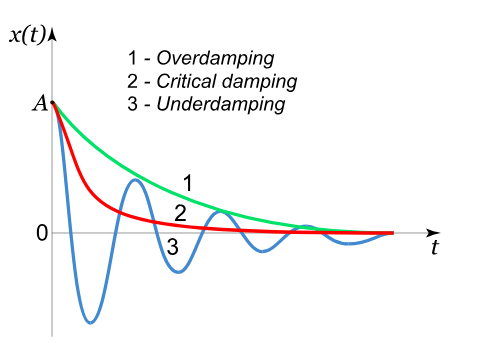
\includegraphics[scale=0.5]{damping.png}


\chapter{Solving Non-homogeneous Linear Differential Equations}
\section{Introduction}
In the previous sections, we mostly focused on the homogeneous case of linear differential equations. In this case we will focus on non-homogeneous equations, that is, there is a term in the differential equation that is only dependent on the independent variable. Thus, we will be considering equations in the form:


$$y''(t) + p_1(t)y'(t) + p_0(t)y(t) = g(t)$$

where $y(t)$ is twice differentiable on an interval $I$ and $p_1(t), p_0(t) and g(t)$ are defined and continuous in this interval.

You can imagine $g(t)$ to be some external force that doesn't depend on our original system (only on time). We will use this fact to study the effect of putting an external force on the spring-mass-dashpot system we talked about before.

\section{Finding the Non-Homogeneous Solution}

The following theorem gives us the method of finding a non-homogeneous solution for a differential equation:

\begin{mytheo}{Non-homogeneous Linear Solution}{nhSol}
 For a non-homogeneous solution of the form
 $$y^{(n)}(t) + ... + p_1(t)y'(t) + p_0(t)y(t) = g(t)$$
 where the coefficients are continuous over an interval $I$, the solution is of the form
 $$\phi(t) = y_h(t) + y_p(t)$$
 where $y_h(t)$ is the complete solution to homogeneous differential equation:
 $$y^{(n)}(t) + ... + p_1(t)y'(t) + p_0(t)y(t) = 0$$
 and $y_p(t)$ is just any particular solution to the original non-homogeneous differential equation.
\end{mytheo}

\hyperref[sec:prNhSol]{The proof is given in the appendix}

This theorem is saying that in order for us to find the solution to a non-homogeneous differential equation we simply need to:
\begin{enumerate}
    \item Find the solutions to the homogeneous case
    \item Find just one function that satisfies our initial non-homogeneous differential equation
    \item Add these solutions together
\end{enumerate}


\section{Non-homogeneous Equation with Constant Coefficients and Exponential Response}

Consider the case we did in the chapter above, a differential equation with constant coefficients. However, this time, let's add a an exponential term only dependant on $t$, so our equation will look like:

$$y^{(n)}(t) + ... + a_1y'(t) + a_0y(t) = be^{\omega t}$$

where $b$ is just a constant value.

As we discussed in the section above, the complete solution to this differential equation is the complete set of all homogeneous solutions plus one particular solution:
$$y(t) = y_h(t) + y_p(t)$$

Using the methods we discussed in the previous chapter, we can solve for the homogeneous solution by finding the roots of the characteristic polynomial for the homogeneous differential equation:

$$y^{(n)}(t) + \dots + a_1y'(t) + a_0y(t) = 0$$

However, how do we go about finding one particular solution?

What happens if we try plugging in $ce^{\omega t}$ as our solution, where $c$ is just an arbritrary constant. Thus we should get:

$$(ce^{\omega t})^{(n)} + \dots + a_1(ce^{\omega t})' + a_0(ce^{\omega t}) = be^{\omega t}$$

Using the fact that the derivative of an exponent is itself and the linearity of the derivative operator, we see that:
$$(\omega^n + \dots + a_1\omega + a_0)ce^{\omega t} = be^{\omega t}$$

We know that $e^{\omega t}$ is never 0 so we can divide both sides by it:
$$(\omega^n + \dots + a_1\omega + a_0)c = b$$

If we suppose that $\omega^n + \dots + a_1\omega + a_0 \neq 0$ (which is in fact a big assumption), we see that we can solve for c:

$$c = \frac{b}{\omega^n + \dots + a_1\omega + a_0}$$

Thus, we have found a particular solution!:

$$y_p(t) =  \frac{b}{\omega^n + \dots + a_1\omega + a_0}e^{\omega t}$$

If we represent the characteristic polynomial as a function:

$$P(r) = r^n + \dots + a_1r + a_0$$

We see that the denominator of our solution is just the characteristic polynomial evaluated at $\omega$.

Thus more compactly, the particular solution is:

$$y_p(t) = \frac{b}{P(\omega)} e^{\omega t}$$
if $P(\omega) \neq 0$



Thus:

\begin{mytheo}{Exponential Response Formula}{ERF}
    For a non-homogeneous differential equation in the form:
    $$y^{(n)}(t) + \dots + a_1y'(t) + a_0y(t) = be^{\omega t}$$
    and the characteristic polynomial
    $$P(r) = r^n + \dots + a_1r + a_0$$
    
    A particular solution to this differential equation is:
    
    $$y_p(t) = \frac{b}{P(\omega)} e^{\omega t}$$
    if $P(\omega) \neq 0$
    
 
\end{mytheo}

What do we do in the specific case of a $\omega_0$ where $P(\omega_0) = 0$? We can evaluate the limit as we approach the value the particular solution

$$y_p(t) = \lim_{\omega \to \omega_0}\frac{b}{P(\omega)} e^{\omega t}$$

We can use L'Hopital's Rule to help evaluate this limit when it is in fact indeterminate $P(\omega_0) = 0$.

L'Hopital's Rule (not stated formally) says that if the function composed of the division of two other functions is indeterminant at some point $x_0$ we can evaluate the limit at the derivatives of both of these functions instead provided the functions are differentiable.

Thus,
if $P(\omega_0) = 0$, but $P'(\omega_0) \neq 0$, then:

$$y_p(t) = \lim_{\omega \to \omega_0}\frac{b}{P(\omega)} e^{\omega t} = \frac{b}{P'(\omega)} te^{\omega t}$$

If $P'(\omega_0) = 0$ also, but the second derivative is non-zero then:

$$y_p(t) = \lim_{\omega \to \omega_0}\frac{b}{P(\omega)} e^{\omega t} = \frac{b}{P''(\omega)} t^2e^{\omega t}$$


and so on.

Thus:

\begin{mytheo}{Generalized Exponential Response Formula}{GERF}
    For a non-homogeneous differential equation in the form:
    $$y^{(n)}(t) + \dots + a_1y'(t) + a_0y(t) = be^{\omega t}$$
    and the characteristic polynomial
    $$P(r) = r^n + \dots + a_1r + a_0$$
    
    At the first non-zero value of $P(r)$ evaluated at $\omega$ (say at the m'th derivative), $P^{m}(\omega) \neq 0$ then we can always find a particular solution by:
    
    $$y_p(t) = \frac{b}{P^{(m)}(\omega)} t^me^{\omega t}$$
    if $P^{(m)}(\omega) \neq 0$
    and all the lower derivatives $P(\omega), P'(\omega), \dots, P^{(m-1)} = 0$
    
 
\end{mytheo}

\section{Complexification for sines and cosines}

The method above only works for exponentials. However, by using Euler's formula:

$$\cos(\omega t) + i\sin(\omega t) = e^{i\omega t}$$

we can use the same method for sinusoidal functions.

Imagine that we have the differential equation:

$$y^{(n)}(t) + \dots + a_1y'(t) + a_0y(t) = b\cos(\omega t)$$

Say that we make a new function such that:
$$z(t) = y(t) + iq(t) $$

In other words: $y(t) = \Re[z(t)]$

Thus, plugging it into the LHS of the equation we get:

$$z(t)^{(n)}(t) + \dots + a_1z'(t) + a_0z(t)$$
$$=(y(t) + iq(t))^{(n)} + \dots + a_1(y(t) + iq(t))' + a_0(y(t) + iq(t))$$

which by linearity gives us:

$$y^{(n)}(t) + \dots + a_1y'(t) + a_0y(t) + i(q^{(n)}(t) + \dots + a_1q'(t) + a_0q(t))$$

Hmm... The first part of this expression looks a lot like the differential equation we originally were trying to solve and if we plug in our original value for it, we get:

$$b\cos(\omega t) + i(q^{(n)}(t) + \dots + a_1q'(t) + a_0q(t))$$

Remember we arbitrarily introduce the function $q(t)$ so we can set the value of it to whatever we want. Say we set $q^{(n)}(t) + \dots + a_1q'(t) + a_0q(t))$ to $\sin(\omega t)$:

We get:

$$b(\cos(\omega t) + i\sin(\omega t))$$

which by Euler's formula is:

$$be^{i\omega t}$$

Thus,
$$z^{(n)}(t) + \dots + a_1z'(t) + a_0z(t) = be^{i\omega t}$$

where $y(t) = \Re[z(t)]$

We know how to solve for $z_p(t)$ using the methods we discussed above! We just need to get the real part of it to solve for our original differential equation.

We can apply the same procedure for a differential equation where instead of cosine, we had sine. We would just solve the complexified equation and take the imaginary part of the solution.

This gives us the method of complexification:

\begin{mytheo}{Complexification}{complexification}
    For a non-homogeneous differential equation with constant coefficien569+ts, if we have a sinusoidal input in the form:
    $$y^{(n)}(t) + \dots + a_1y'(t) + a_0y(t) = b\cos(\omega t)$$
    or 
    $$y^{(n)}(t) + \dots + a_1y'(t) + a_0y(t) = b\sin(\omega t)$$
    We can find a particular solution for these cases if we solve a different differential equation:
    $$z^{(n)}(t) + \dots + a_1z'(t) + a_0z(t) = be^{i\omega t}$$
    which we can solve using the \hyperref[th:GERF]{Generalized ERF.}
    
    To find the solutions for our differential equation we take Real or Imaginary part of the solution $z_p(t)$. Thus in the first case with cosine:
    $$y_p(t) = \Re{z_p(t)}$$
    In the second case with sine:
    $$y_p(t) = \Im{z_p(t)}$$
\end{mytheo}

\section{Constant Coefficients with a Polynomial Response}
Let's say that we're given the differential equation

$$y^{(n)}(t) + \dots + c_1y'(t) + c_0y(t) = a_0t^n + a_1t^{n-1} + \dots a_n$$

(Notice that I switched $a_0 \dots a_n$ with $c_n \dots  c_0$. I did this because of convention in a lot of textbooks)

It turns out that we can find the solution for this case:

\begin{mytheo}{Polynomial Response}{polyResp}
    Given a non-homogeneous differential equation with constant coefficients of the form:
    $$y^{(n)}(t) + \dots + c_1y'(t) + c_0y(t) = a_0t^n + a_1t^{n-1} + \dots a_n$$
    
    A particular solution will take the form:
    
    $$y_p(t) = A_0t^n + \dots + A_n$$
    if $c_0 \neq 0$:
    
    If $c_0=0$, then the form will be:
    
    $$y_p(t) = t(A_0t^n + \dots + A_n)$$
    if $c_1 \neq 0$:
    
    If both $c_0=c_1=0$, then the particular solution will be:
    $$y_p(t) = t^2(A_0t^n + \dots + A_n)$$
    if $c_2 \neq 0$:

    This process continues on. Thus when we have $c_0 = c_1 = \dots = c_s = 0$, the form of a particular solution is:
    $$y_p(t) = t^{s+1}(A_0t^n + \dots + A_n)$$
    if $c_{s+1} \neq 0$:
    
\end{mytheo}

\hyperref[sec:prPolyResp]{The proof of this is given in the appendix.}


After we know the form of a particular solution, it is relatively straightforward to go about finding the actual coefficients. We can just plug it into our equation and relate like terms together.

\section{Method of Undetermined Coefficients}
We might run into a specific case of a differential equation where the response is in fact a sum or product of an exponential and polynomial. How do we deal with those cases to find a particular solution?

Let's start with sums:

This theorem applies in general (doesn't require terms to be polynomials or exponentials):

\begin{mytheo}{Particular Solution to Sum of different responses}{sumResp}
    Given a differential equation in the form of:
    $$y^{(n)}(t) + \dots + c_1y'(t) + c_0y(t) = g_1(t) + \dots + g_m(t)$$
    and given that we have a particular solution for the differential equations:
    $$y^{(n)}(t) + \dots + c_1y'(t) + c_0y(t) = g_1(t)$$
    $$\vdots$$
    $$y^{(n)}(t) + \dots + c_1y'(t) + c_0y(t) = g_m(t)$$
    which we will denote as $y_1(t), \dots, y_m(t)$ respectively.
    
    A particular solution to the original differential equation can be found by taking the sum of these particular solutions:
    $$y_p(t) = y_1(t) + \dots + y_m(t)$$
    
\end{mytheo}

The proof of this fact is relatively simple and relies on the linearity of the problem (almost exactly the same proof as for homogeneous differential equations).


\section{Method of Variation of Parameters}
The method of variation of parameters allows us a method for determining the solution to an non-homogeneous n'th order linear differential equation, provided we know all of the homogeneous solutions.

\begin{mytheo}{Variation of Parameters}{var}
    Say we have a differential equation of the form:

    $$y^{(n)}(t) + \dots + p_1(t)y'(t) + p_0(t)y(t) = g(t)$$

    Say that the n solutions to the homogeneous are:
    $y_1(t), y_2(t), \dots, y_n(t)$ respectively.
    
    We can always find a particular solution to the non-homogeneous differential equation above by:
    
    $$y_p(t) = u_1(t)y_1(t) + u_2(t)y_2(t) + \dots + u_n(t)y_n(t)$$
    
    where the functions $u_1(t), \dots, u_n(t)$ can be determined by computing the derivatives by:
    
    
$$
\begin{bmatrix}
    u_1'(t) \\
    u_2'(t) \\
    \vdots \\ 
    u_n'(t)
\end{bmatrix}
=
\begin{bmatrix}
    y_1(t) & y_2(t) & \dots  & y_n(t) \\
    y_1'(t) & y_2'(t) & \dots  & y_n'(t) \\
    \vdots & \vdots & \ddots & \vdots \\
    y_1^{(n)}(t) & y_2^{(n)}(t) & \dots  & y_n^{(n)}(t) \\
\end{bmatrix}^{-1}
\begin{bmatrix}
    0 \\
    0 \\
    \vdots \\ 
    g(t)
\end{bmatrix}
$$
Once we have the derivatives, we can integrate to find the actual functions $u_1(t), \dots, u_n(t)$
\end{mytheo}

\hyperref[sec:prVar]{The (lengthy) proof is in the appendix.}

This gives us a general way to solve for a particular solution of any non-homogeneous linear differential equation given we know the homogeneous solutions! 

\section{Application: Resonance}
Imagine a spring-mass system we discussed earlier without damping. What if we applied a sinusoidal force to our oscillator?

Thus,
$$F = -kx + A\cos(\omega t)$$
$$\dv[2]{x}{t} + \frac{k}{m}x = A\cos(\omega t)$$

This is a non-homogeneous differential equation. If we use the ERF to solve for a particular solution, we get:

$$x_p(t) = \frac{A\cos(\omega t)}{(k/m)^2-\omega^2}$$

if $\frac{k}{m} \neq \omega$

However, something interesting happens as $\omega$ is in fact the natural frequency $\frac{k}{m}$. We can see that as it approaches this value, we get higher and higher values for x. We can use l'Hopital's rule to determine the exact value of this limit which is:

$$\lim_{\omega \to k/m}(\frac{A\cos(\omega t)}{(k/m)^2-\omega^2}) = \frac{At\sin(\omega t)}{2\omega}$$


Notice that now the response is in fact a sinusoidal function with increasing amplitude!

This phenomenon is called \textbf{pure resonance}





\chapter{Linear Systems of Differential Equations}
\section{Introduction}
Linear systems of differential equations become important when we want to model rates of change that depend on multiple variables and those variables further depend on other variables.

For example (and oversimplifying greatly), the rate of change in the population of wolfs in a forest may depend on the current population of wolfs and the population of their prey (such as deer). The rate of change in the deer population also depends on the population of predators and the current population of deer. Therefore we could model the system as:

$$x' = ax + by$$
$$y' = cx + dy$$

This can also be thought of in matrix form:

$$
\begin{bmatrix}
    x' \\
    y' \\
\end{bmatrix}
=
\begin{bmatrix}
    a & b \\
    c & d \\
\end{bmatrix}
\begin{bmatrix}
    x \\
    y \\
\end{bmatrix}
$$

We will discuss how to solve such matrices and understand the long term behaviour of systems like these.

In this chapter we will use the convention that for each variable $x_i$, we will not put $(t)$ afterward to represent a function (even though it is in fact a function).

\section{Existence of Solutions}
In this section, we will consider the system of differential equation as follows:

$$x_1' = F_1(x_1, \dots, x_n)$$
$$\vdots$$
$$x_n' = F_2(x_1, \dots, x_n)$$

We define a \textbf{solution} to this differential equation when we have:

$$x_1 = \phi_1(t)$$
$$\vdots$$
$$x_n = \phi_n(t)$$

defined on some interval $I$ where the solutions are differential and satisfy the initial system of equations.

There is an Existence and Uniqueness Theorem for systems of differential equations as well:

\begin{mytheo}{Existence and Uniqueness Theorem for System}{exUnSys}
    For the system of differential equation:
    $$x_1' = F_1(x_1, \dots, x_n)$$
    $$\vdots$$
    $$x_n' = F_2(x_1, \dots, x_n)$$
    
    If $F_1, \dots F_n$  and all of the partial derivatives of $F_1, \dots F_n$ with respect to $x_1, \dots x_n$ ($n^2$ total partial derivatives) are continuous on some region $R$ of $t, x_1, \dots, x_n$. 
    
    Furthermore say that at some point in R, say
    $t_0, x_1^0, \dots x_n^0$, some initial constraint is satisfied:
    $$x_1(t_0) = x_1^0$$
    $$\vdots$$
    $$x_n(t_0) = x_n^0$$
    
    Then there must exist a unique solution on some interval I for which $x_1 = \phi_1(t), \dots, x_n = \phi_n(t)$ such that both the initial system and the initial conditions are satisfied.
    
\end{mytheo}

The proof of this theorem is not given.

Note one thing: the partial derivatives of $F_1, \dots, F_n$ with respect to $t$ are irrelevant in deciding if we can find a solution or not.


Just like in the case of $n'th$ order differential equations, there are both linear can non-linear cases.

A \textbf{linear} system of differential equations is one where each function $F_1, \dots, F_n$ are combinations of $x_1, \dots, x_n$ such that the coefficients only depend on time. Thus a linear system of equations looks like:


$$x_1' = p_{11}(t)x_1 + \dots + p_{1n}(t)x_n +g_1(t)$$
$$\vdots$$
$$x_n' = p_{n1}(t)x_1 + p_{nn}(t)x_n + g_n(t)$$

We will be dropping the $(t)$ for the functions $p_11(t), \dots, p_nn(t)$ and $g_1(t), \dots, g_n(t)$ in future discussions.

Another way of viewing linear systems is that we can represent them in matrix form:


$$
\begin{bmatrix}
    x_1' \\
    \vdots \\
    x_n' \\
\end{bmatrix}
=
\begin{bmatrix}
    p_{11} &  \dots & p_{1n} \\
    \vdots & \ddots & \vdots \\
    p_{n1} &  \dots & p_{nn} \\
\end{bmatrix}
\begin{bmatrix}
    x_1 \\
    \vdots \\
    x_n \\
\end{bmatrix}
+
\begin{bmatrix}
    g_1 \\
    \vdots \\
    g_n \\
\end{bmatrix}
$$

which is also:

$$\mathbf{x}' = \mathbf{Px} + \mathbf{g}$$

where bold letters represent matrices

If $\mathbf{g} = \mathbf{0}$, we call it a \textbf{homogeneous} system of differential equation and if it is non-zero it is \textbf{non-homogeneous}.


If $p_{11}, \dots, p_{nn}$ and $g_1, \dots, g_n$ are continuous, then there exists a unique solution for some initial conditions.

Why?
Since the partial derivatives of all of the $F_1, \dots, F_n$ of a linear system of differential equation are in fact $p_11, \dots p_nn$, we can just check the continuity of these functions to satsisfy the Existence and Uniqueness Theorem.



Let's consider the case of a linear, homogeneous system:


$$\mathbf{x}' = \mathbf{Px}$$


(Note on convention:
We will denote solutions by $\mathbf{x}^{(1)}, \dots \mathbf{x}^{(n)}$. In addition, the solution vectors components will be labelled as:

$$\mathbf{x}^{(j)} = 
\begin{bmatrix}
    x_1^{(j)} \\
    \vdots \\
    x_n^{(j)} \\
\end{bmatrix}
$$
)

The following theorem is very similar to that of superposition for $n$'th order differential equations:

\begin{mytheo}{Sum of Two Homogeneous Solutions}{sysSum}
    If $\mathbf{x}^{(1)}$ and $\mathbf{x}^{(2)}$ are both solutions to the some homogeneous system in the form of
    $$\mathbf{x}' = \mathbf{Px}$$
    than any linear combination of these two solutions is also a solution.
    $$\mathbf{x}^{(3)} = c_1\mathbf{x}^{(1)} + c_2\mathbf{x}^{(2)}$$
\end{mytheo}


This applies again, just like the $n$'th order case because taking derivatives is a linear operator.

This begs the question we had in the $n$'th order case, how do we know we have enough solutions to span the solution space?

Just like before, we know that we have enough solution vectors $\mathbf{x}^{(1)}, \dots, \mathbf{x}^{(n)}$ if and only if for any $n$ set of initial conditions $x_1(t_0) = x_1^0, \dots, x_n(t_0) = x_n^0$ we can find a unique solution.

By the principle of superposition, we know that any solution can be composed of a linear combination of other solutions.

Imagine if we could find some solutions $\mathbf{x}^{(1)}. \dots, \mathbf{x}^{(n)}$ such that we could always find a linear combination such that we solve for the unique solution for \textbf{any} initial value problem:

$$
\begin{bmatrix}
    \vert & & \vert \\
    \mathbf{x}^{(1)}(t_0) & \dots & \mathbf{x}^{(n)}(t_0) \\
    \vert & & \vert \\
\end{bmatrix}
\begin{bmatrix}
    c_1 \\
    \vdots \\
    c_n \\
\end{bmatrix}
=
\begin{bmatrix}
    x_1^0 \\
    \vdots \\
    x_n^0 \\
\end{bmatrix}
$$

If $\mathbf{x}^{(1)}. \dots, \mathbf{x}^{(n)}$ are in fact our basis solutions than we should be able to find a unique $c_1, \dots, c_n$ that solve this system:

$$
\begin{bmatrix}
    c_1 \\
    \vdots \\
    c_n \\
\end{bmatrix}
=
\begin{bmatrix}
    \vert & & \vert \\
    \mathbf{x}^{(1)}(t_0) & \dots & \mathbf{x}^{(n)}(t_0) \\
    \vert & & \vert \\
\end{bmatrix}^{-1}
\begin{bmatrix}
    x_1^0 \\
    \vdots \\
    x_n^0 \\
\end{bmatrix}
$$


Let's put some names to things:

$$\mathbf{X(t)} = 
\begin{bmatrix}
    \vert & & \vert \\
    \mathbf{x}^{(1)}(t) & \dots & \mathbf{x}^{(n)}(t) \\
    \vert & & \vert \\
\end{bmatrix}
$$

$$
\mathbf{c} = 
\begin{bmatrix}
    c_1 \\
    \vdots \\
    c_n \\
\end{bmatrix}
$$

$$
\mathbf{x^0} =
\begin{bmatrix}
    x_1^0 \\
    \vdots \\
    x_n^0 \\
\end{bmatrix}
$$

Therefore, the following theorem must hold:


\begin{mytheo}{Fundamental Set of Solutions}{fundSys}
For a system of linear differential equations:

$$\mathbf{x'} = \mathbf{Px}$$

If we solve for $n$ solutions 
$\mathbf{x}^{(1)}, \dots, \mathbf{x}^{(n)}$ such that:

$$\mathbf{X(t)} = 
\text{det}\left(\begin{bmatrix}
    \vert & & \vert \\
    \mathbf{x}^{(1)}(t_0) & \dots & \mathbf{x}^{(n)}(_0t) \\
    \vert & & \vert \\
\end{bmatrix}\right)
\neq 0
$$

then the solutions $\mathbf{x}^{(1)}, \dots, \mathbf{x}^{(n)}$ form \textbf{fundamental set of solutions} such that we can we can solve for any unique solution to an IVP by taking a linear combination of these solutions. In addition, the matrix formed by taking the columns of the $n$ solutions is called the \textbf{Wronskian}.

\end{mytheo}

Notice how the Wronskian appears again! This time, instead of using the matrix formed by taking the derivatives of a set of solutions over again, it is formed by just putting the solutions as column vectors.

Another interesting parallel to the $n'th$ order differential equation case is:

\begin{mytheo}{Wronskian General Form}{wronAbelSys}
    For a system of differential equations defined in some interval $I$ in the form:
    $$\mathbf{x'} = \mathbf{Px}$$
    
    For any $n$ solutions $\mathbf{x}^{(1)}, \dots, \mathbf{x}^{(n)}$
    
    the Wronskian will satisfy the following differential equation:
    
    $$\dv{W}{t} = (p_11 + \dots + p_nn)W$$
    
    Solving this gives us the general form of the Wronskian:
    
    $$W = c\exp{\int{p_{11} + \dots + p_{nn})dt}}$$
\end{mytheo}
This is a parallel to Abel's Theorem!!

\hyperref[sec:wronAbelSys]{The proof of this for a system of two equations is given in the appendix.}

This directly implies the following:

\begin{mytheo}{Wronskian over interval for solutions}{wronOverI}
    For any set of solutions $\mathbf{x}^{(1)}, \dots, \mathbf{x}^{(n)}$, the Wronskian is either always 0 or never 0.
\end{mytheo}


















\section{Homogeneous Solutions of a System of Differential Equation}
How do we go about finding the solutions to a homogeneous system of differential equations in the form of a system:

$$\mathbf{x'} = \mathbf{Px}$$

Since we see the expression $x'$ on the left and $x$ on the right, we might guess that this has something vaguely to do with exponentials.

Let's try guessing something of the form:

$$\mathbf{x} = \mathbf{v}e^{\lambda t}$$

where $\mathbf{v}$ is just some vector.

Plugging this in, we get:

$$(\mathbf{v}e^{\lambda t})' = \mathbf{Pv}e^{\lambda t}$$

Since $\mathbf{v}$ is just a constant, we can simplify this to:

$$\mathbf{v}\lambda e^{\lambda t} =  \mathbf{Pv}e^{\lambda t}$$

Since $e^{\lambda t}$ is never 0, we can divide both sides by it:

$$\mathbf{v}\lambda =  \mathbf{Pv}$$

Rearranging terms, we have:

$$\mathbf{Pv} = \lambda\mathbf{v}$$

From linear algebra, we know that this can be solved by the eigenvectors and eigenvalues of $\mathbf{P}$!

Thus, our solutions are constrained by values:

$$\text{det}(\mathbf{P} - \lambda\mathbf{I}) = 0$$

Taking the determinant of the expression above gives us some polynomial of $n$'th degree in $\lambda$, and thus we have 3 different cases:

\begin{enumerate}
    \item Eigenvalues are are all real and unique.
    \item Eigenvalues are in complex conjugate pairs
    \item Eigenvalues are repeated
\end{enumerate}

\subsection{Real and Unique Eigenvalues}
If all the eigenvalues are real and unique, then we have $n$ linearly independent eigenvectors associated with each eigenvalue. Therefore, we can find $n$ linearly independent solutions:


$$ \mathbf{x_1}(t)=\mathbf{v_1}e^{\lambda_1 t}$$
$$\vdots$$
$$ \mathbf{x_n}(t)=\mathbf{v_n}e^{\lambda_n t}$$

We can put these solutions as columns and take the determinant to verify that the Wronskian is in fact non-zero everywhere.

Thus, we have a fundamental set of solutions!!

Our general solution will be in the form:

$$ \mathbf{x}(t) = c_1\mathbf{v_1}e^{\lambda_1 t} + \dots + \mathbf{v_n}e^{\lambda_n t}$$



\subsection{Complex Conjugate Pairs of Eigenvalues}
Suppose we get complex eigenvalues for the following system:

$$(\mathbf{P} - \lambda\mathbf{I})\mathbf{v} = \mathbf{0}$$

Let's take the complex conjugate of both sides:

$$\overline{(\mathbf{P} - \lambda\mathbf{I})\mathbf{v}} = \overline{\mathbf{0}}$$

If $\mathbf{P}$ is real, this simplifies to:

$$(\mathbf{P} - \overline{\lambda}\mathbf{I})\overline{\mathbf{v}}= \mathbf{0}$$

which is another eigenvalue, eigenvector pair. Thus, the following holds:

\begin{mytheo}{Complex Eigenvectors and Eigenvalues come in pairs}{compEigen}
    If the eigenvalue of some matrix is complex, $\lambda_1 = a + ib$, for some real $a,b$ and the eigenvector associated with this eigenvector is $\mathbf{v_1}$, then there we can always find a second eigenvalue, eigenvector combination 
    $$\lambda_2 = \overline{\lambda_1} = a - ib$$
    $$\mathbf{v_2} = \overline{\mathbf{v_1}}$$
\end{mytheo}


Thus, if we have the solution:

$$\mathbf{x_1}(t)=\mathbf{v_1}e^{(a+bi) t}$$
then another solution is formed by:
$$\mathbf{x_2}(t)=\overline{\mathbf{v_1}}e^{(a-bi) t}$$

We also know that the real and imaginary part of a number is:

$$\Re{x} = \frac{x+\overline{x}}{2}$$
$$\Im{x} = \frac{x-\overline{x}}{2i}$$

In our case:
$$\Re{\mathbf{x_1}(t)} = \frac{\mathbf{x_1}(t)+\overline{\mathbf{x_1}(t)}}{2}=\frac{\mathbf{x_1}(t)+\mathbf{x_2}(t)}{2}$$

and:
$$\Im{\mathbf{x_1}(t)} = \frac{\mathbf{x_1}(t)-\overline{\mathbf{x_1}(t)}}{2i}=\frac{\mathbf{x_1}(t)-\mathbf{x_2}(t)}{2i}$$

Notice that since the real and imaginary parts of the solution of $\mathbf{x_1}(t)$ are in fact linear combinations of two solutions, they are in fact solutions themselves!! They also end up being real solutions.

Thus:
\begin{mytheo}{Solution to Complex Eigenvalues}{compEigenvals}
    Say we are solving the equation:
    $$\mathbf{x'} = \mathbf{Px}$$
    and we plug in a solution of the form:
    $$\mathbf{x} = \mathbf{v}e^{\lambda t}$$
    and solve for the corresponding eigenvalue equation and get a complex conjugate pair for the eigenvalues and eigenvectors.
    
    We can find two solutions to this complex pair by taking the real and imaginary part of one solution formed by the complex eigenvalue-eigenvector pair:
    
    $$\mathbf{x_1(t)} = \Re{\mathbf{v_1}e^{\lambda_1 t}}$$
    $$\mathbf{x_2(t)} = \Im{\mathbf{v_1}e^{\lambda_1 t}}$$
    
    where both $\lambda_1$ and $\mathbf{v_1}$ are complex
\end{mytheo}

\subsection{Repeated Eigenvalues}
\label{sec:repEigen}
What happens when we get some repeated eigenvalues?

Well, there are two situations that can arise. One is where we still can get out linearly independent eigenvectors out of the same repeated eigenvalue.

So for example, if we have the matrix $\lambda\mathbf{I}$:
$$
\begin{bmatrix}
    \lambda & 0  \\
    0 & \lambda  \\
\end{bmatrix}
$$

There is just one eigenvalue $\lambda$. However, there are two linearly indepedent eigenvectors that can be formed 

$$
\mathbf{v_1}
=
\begin{bmatrix}
    1 \\
    0 \\
\end{bmatrix},
\mathbf{v_2}
=
\begin{bmatrix}
    0 \\
    1 \\
=\end{bmatrix},
$$

Thus, in this case, we can proceed as before as we did in the real and unique eigenvalue case.

However, what if we get a matrix like:

$$
\begin{bmatrix}
    1 & 1  \\
    0 & 1  \\
\end{bmatrix}
$$

In this case, there is only one eigenvalue, $\lambda = 1$. However, we \textbf{cannot} extract multiple linearly independent eigenvectors. There is only one eigenvector in this case:

$$
\mathbf{v_1}
=
\begin{bmatrix}
    1 \\
    0 \\
\end{bmatrix},
$$

What should we do in this case to find another linearly independent solution?


Say we have the system:

$$\mathbf{x'} = \mathbf{Px}$$

Say that we extracted one eigenvalue and one non-zero eigenvector, but we're trying to find another solution. We know for sure, that one solution can be given by:

$$\mathbf{x_1}(t) = \mathbf{v_1}e^{\lambda_1 t}$$

For the second solution let's try just multiplying by $t$:

$$\mathbf{x_2}(t) \stackrel{?}{=} \mathbf{v_1}te^{\lambda_1 t}$$


Plugging this into our original system, we get:

$$(\mathbf{v_1}te^{\lambda_1 t})' = \mathbf{P}\mathbf{v_1}te^{\lambda_1 t}$$

Using the chain rule and eigenvector properties, we get:

$$\mathbf{v_1}e^{\lambda_1 t} + \lambda_1\mathbf{v_1}te^{\lambda_1 t} = \lambda_1 \mathbf{v_1}te^{\lambda_1 t}$$

which gives us:
$$\mathbf{v_1}e^{\lambda_1 t} = 0$$
which after simplifying more gives us:
$$\mathbf{v_1} = 0$$

This is contradiction, since we assumed $\mathbf{v_1}$ was non-zero to begin with! Thus, our guess was incorrect :(


Hmm..., looking at how the "solution" failed above, we see that on the LHS that there is both a $te^{\lambda_1 t}$ and $e^{\lambda_1 t}$ component. Thus, let's try to guess:


$$\mathbf{x_2}(t) \stackrel{?}{=} \mathbf{v_1}te^{\lambda_1 t} + \mathbf{v_2}e^{\lambda_1 t}$$

where $\mathbf{v_2}$ is an arbitrary vector.

Plugging this into our original system, we get:


$$(\mathbf{v_1}te^{\lambda_1 t} + \mathbf{v_2}e^{\lambda_1 t})' = \mathbf{P}(\mathbf{v_1}te^{\lambda_1 t} + \mathbf{v_2}e^{\lambda_1 t})$$

Simplifying this expression using the chain rule:

$$\mathbf{v_1}e^{\lambda_1 t} + \lambda_1\mathbf{v_1}te^{\lambda_1 t} + \lambda_1\mathbf{v_2}e^{\lambda_1 t} = \mathbf{P}\mathbf{v_1}te^{\lambda_1 t} + \mathbf{P}\mathbf{v_2}e^{\lambda_1 t}$$

Using the fact that $\mathbf{P}\mathbf{v_1} = \lambda_1\mathbf{v_1}$:

$$\mathbf{v_1}e^{\lambda_1 t} + \lambda_1\mathbf{v_1}te^{\lambda_1 t} + \lambda_1\mathbf{v_2}e^{\lambda_1 t} = \lambda_1\mathbf{v_1}te^{\lambda_1 t} + \mathbf{P}\mathbf{v_2}e^{\lambda_1 t}$$

We can subtract both sides by  $\lambda_1\mathbf{v_1}te^{\lambda_1 t}$, to get:

$$\mathbf{v_1}e^{\lambda_1 t} + \lambda_1\mathbf{v_2}e^{\lambda_1 t} = \mathbf{P}\mathbf{v_2}e^{\lambda_1 t}$$

Moving terms and switching sides:
$$\mathbf{P}\mathbf{v_2}e^{\lambda_1 t} - \lambda_1\mathbf{v_2}e^{\lambda_1 t} = \mathbf{v_1}e^{\lambda_1 t}  $$

Since $e^{\lambda_1 t}$ is always greater than 0, we can divide both sides by it:
$$\mathbf{P}\mathbf{v_2} - \lambda_1\mathbf{v_2} = \mathbf{v_1} $$

We can factor out $\mathbf{v_2}$:

$$(\mathbf{P}-\lambda_1\mathbf{I})\mathbf{v_2} = \mathbf{v_1} $$

Also, since $\mathbf{v_1}$ satisfies:

$$(\mathbf{P}-\lambda_1\mathbf{I})\mathbf{v_1} = 0$$

Plugging in the expression for $v_1$ in the above expression:

$$(\mathbf{P}-\lambda_1\mathbf{I})(\mathbf{P}-\lambda_1\mathbf{I})\mathbf{v_2} = 0$$
$$(\mathbf{P}-\lambda_1\mathbf{I})^2\mathbf{v_2} = 0$$


Thus, if we can solve for $\mathbf{v_2}$ using the expression above, we can in fact solve for another linearly independent solution! The vector $\mathbf{v_2}$ is in fact called a \textbf{generalized eigenvector} to the matrix $P$.


It turns out that we can continue this process if the multiplicity of the eigenvalues is greater than 2:

\begin{mytheo}{Repeated Eigenvalues}{repEig}
    Given the system of linear differentiable equations:
    
    $$\mathbf{x'} = \mathbf{Px}$$
    
    If we solve for the eigenvalues of $P$ and get $k$ repeats (multiplicity of $k$), but $< k$ linearly independent eigenvectors, we can find linearly independent solutions by computing the generalized eigenvectors defined by:
    $$(\mathbf{P}-\lambda\mathbf{I})^j\mathbf{v_j} = \mathbf{0} $$
    $$(\mathbf{P}-\lambda\mathbf{I})^{j-1}\mathbf{v_j} \neq \mathbf{0}$$
    for $j = 1, \dots, k$
    such that:
    $$(\mathbf{P}-\lambda\mathbf{I})\mathbf{v_1} = \mathbf{0}$$
    $$(\mathbf{P}-\lambda\mathbf{I})\mathbf{v_2} = \mathbf{v_1}$$
    $$\vdots$$
    $$(\mathbf{P}-\lambda\mathbf{I})\mathbf{v_k} = \mathbf{v_{k-1}}$$
    
    Once we have the generalized eigenvectors, we can find $k$ linearly independent solutions by:
    $$\mathbf{x_1}(t) = \mathbf{v_1}e^{\lambda t}$$
    $$\mathbf{x_2}(t) = (\mathbf{v_2} + t\mathbf{v_1})e^{\lambda t}$$
    $$\vdots$$
    $$\mathbf{x_k}(t) = \left(\mathbf{v_k} + t\mathbf{v_{k-1}} + \frac{t^2}{2}\mathbf{v_{k-2}} + \dots + \frac{t^{(k-1)}}{(k-1)!}\mathbf{v_1}\right)e^{\lambda t}$$
\end{mytheo}



\section{Visualization of 2x2 solutions and Trace-Determinant Plane}

Let's examine how particular solutions to the eigenvalues of a 2x2 coefficient matrix look geometrically:


\subsection{Nodal sources and sinks and saddle points}

In the case of real eigenvalues, our solution will be in the form:

$$\mathbf{x} = \mathbf{v_1}e^{\lambda_1 t} + \mathbf{v_2}e^{\lambda_2 t}$$

What happens geometrically when both $\lambda_1, \lambda_2 > 0$?

If we plot the solution we see that as time goes on, we are repelled from the center at any starting point:

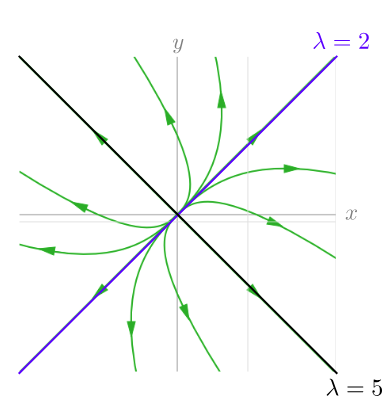
\includegraphics[scale=0.5]{nodal_source.png}

This is called a \textbf{nodal source}

Similarly if $\lambda_1,\lambda_2 < 0$, we get:

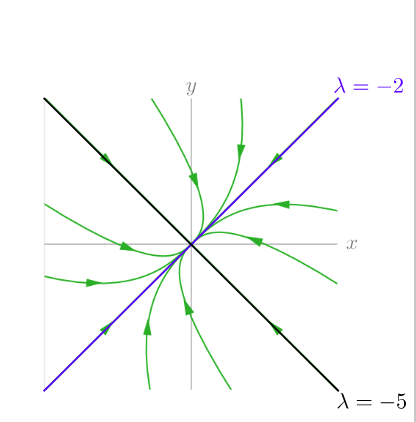
\includegraphics[scale=0.5]{nodal_sink.png}

This is called a \textbf{nodal sink} since as time goes by we go toward the eigenvectors.



If we have opposite signs, we get something called a \textbf{saddle point}:

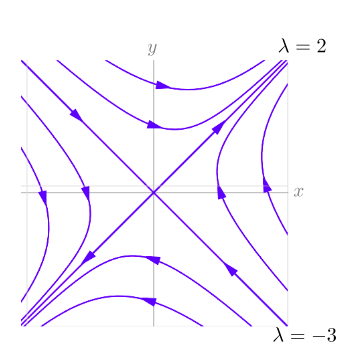
\includegraphics[scale=0.5]{saddle.png}


\subsection{Centers and Spirals}
\label{sec:center}
In this section we will examine the case where we get complex eigenvalues.

\hyperref[sec:prCenter]{The proof of the following fact is given in the appendix.}


In the case of a purely imaginary eigenvalue $\lambda = i\mu$, the complete solution can be described by:

$$
\mathbf{x(t)} = 
\begin{bmatrix}
    A_1\cos(\mu t - \phi_1) \\ 
    A_2\sin(\mu t - \phi_2) \\
\end{bmatrix}
$$

This is just an ellipse! with a center determined by $\phi_1, \phi_2$ and sides $A_1, A_2$. This is called a \textbf{center}:


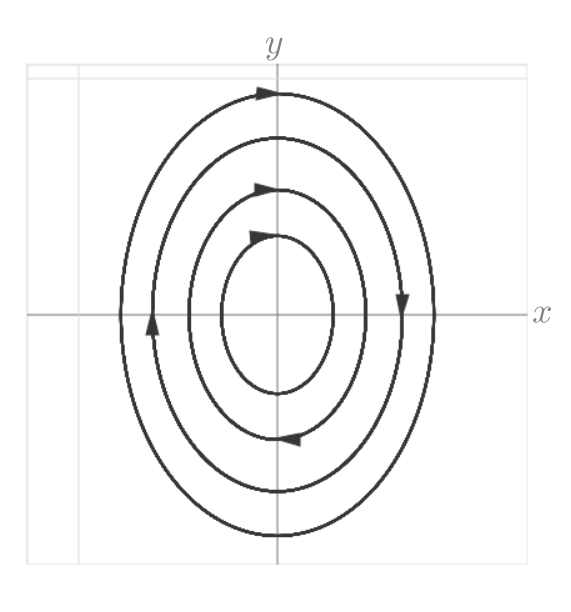
\includegraphics[scale=0.4]{center.png}


What if there is in fact a non-zero real component to the complex eigenvalue?

$$\lambda = r + i\mu$$

Then we have:
$$\mathbf{x(t)} = c_1\Re{\mathbf{v_1}e^{(r+i\mu) t}} + c_2\Im{\mathbf{v_1}e^{(r+i\mu) t}}$$

which is just:


$$\mathbf{x(t)} = e^{rt}[c_1\Re{\mathbf{v_1}e^{i\mu) t}} + c_2\Im{\mathbf{v_1}e^{i\mu t}}]$$


The right side of this expression is identical to before. However, now we have an exponential term to deal with:


$$
\mathbf{x(t)} = 
e^{rt}
\begin{bmatrix}
    A_1\cos(\mu t - \phi_1) \\ 
    A_2\sin(\mu t - \phi_2) \\
\end{bmatrix}
$$

You could think about this as an exponentially increasing or decreasing amplitude for the ellipse. Thus this forms a spiral!

If the eigenvalues are:
$\lambda = r \pm i\mu$ and $r>0$, then we get a \textbf{spiral source}:

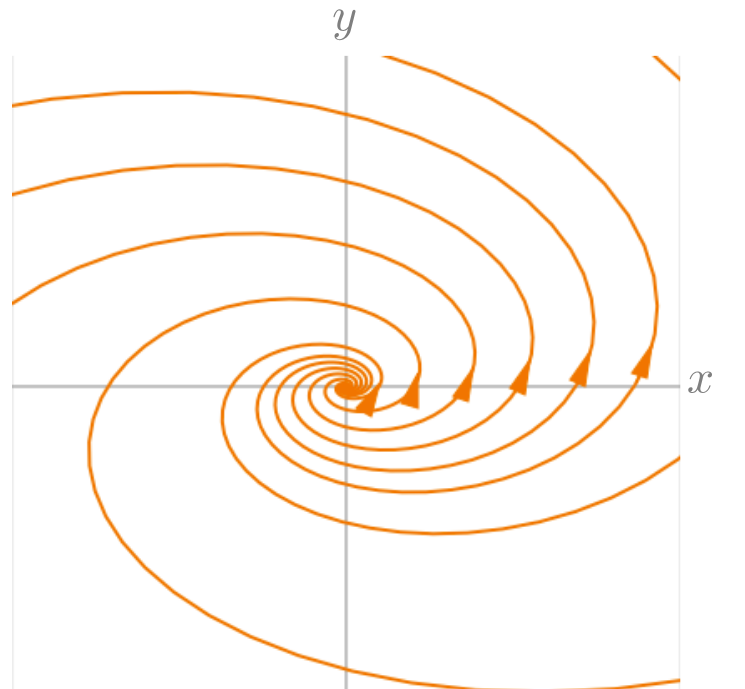
\includegraphics[scale=0.3]{spiral_source.png}


Otherwise if the eigenvalues are:
$\lambda = r \pm i\mu$ and $r<0$, then we get a \textbf{spiral sink}:

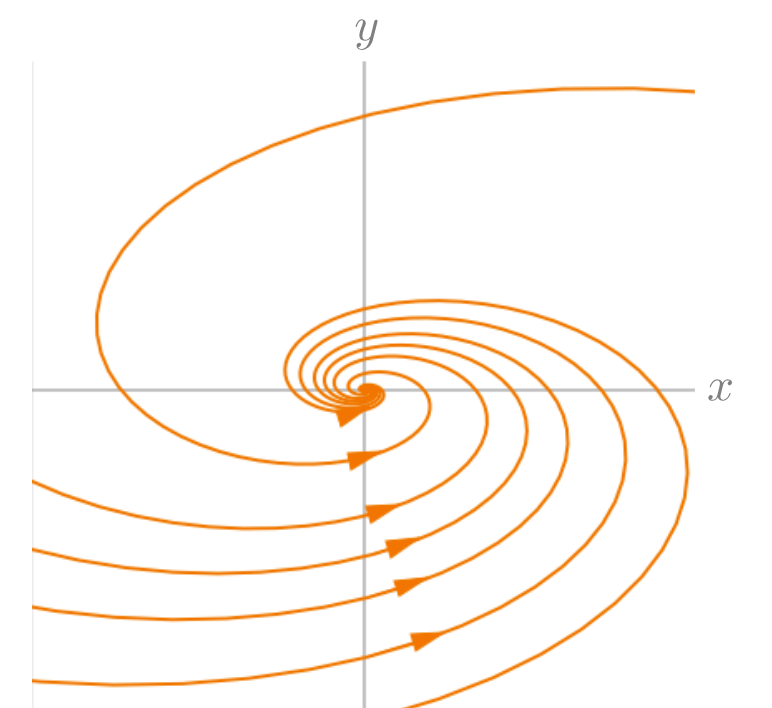
\includegraphics[scale=0.3]{spiral_sink.png}

\subsection{Combs, Degenerate Node and Star Nodes}

What happens when we have one of the eigenvalues to be 0?

We get something like this called a \textbf{comb}. It can be a \textbf{repelling comb} or an \textbf{attracting comb} depending on whether the non-zero eigenvalue is positive or negative respectively (the figure is of attracting comb):.

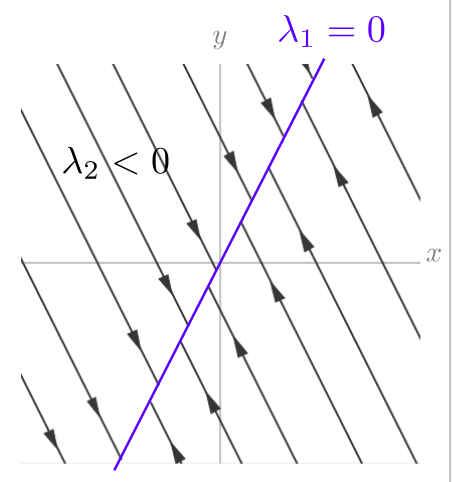
\includegraphics[scale=0.4]{comb.png}

What happens when we have repeated roots?

\hyperref[sec:repEigen]{In our discussion above} we described two cases. One where even though we had $k$ repeated eigenvalues, we were still able to find $k$ linearly independent eigenvectors. It turns out that this is the case when $\mathbf{P} = \lambda I$. Thus the solution will simply be:

$$\mathbf{x}(t) = 
c_1
\begin{bmatrix}
    1 \\
    0
\end{bmatrix}
e^{\lambda t}
+
c_2
\begin{bmatrix}
    1 \\
    0
\end{bmatrix}
e^{\lambda t}
$$

which forms a \textbf{star node} when we plot it:

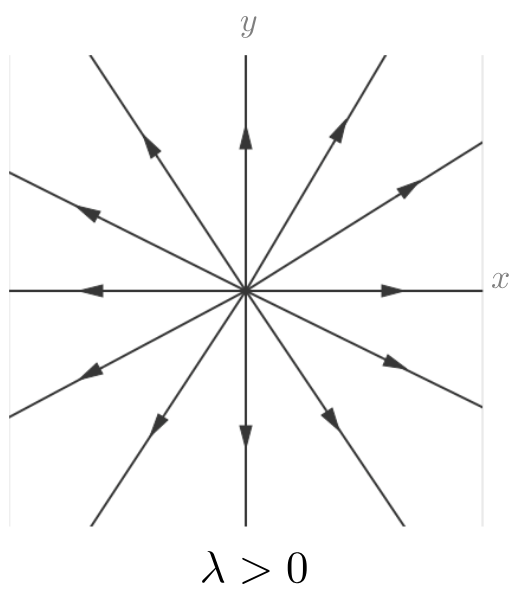
\includegraphics[scale=0.4]{star_node.png}

Notice that this can be attracting or repelling depending on whether or not $\lambda < 0$ or $\lambda > 0$ respectively.

There are some cases, called degenerate cases, where we get repeated eigenvalues without linearly independent eigenvectors. In this case two find the two linearly independent solutions to span the solution space, we need to find the \hyperref[th:repEig]{generalized eigenvectors as described above}.

Thus, the complete solution in this case is given by:

$$\mathbf{x}(t) = c_1\mathbf{v_1}e^{\lambda t} + c_2(t\mathbf{v_1} + \mathbf{v_2})e^{\lambda t}$$

When we plot this out, we see something that looks like it is in between a spiral and a node called a \textbf{degenerate node}:

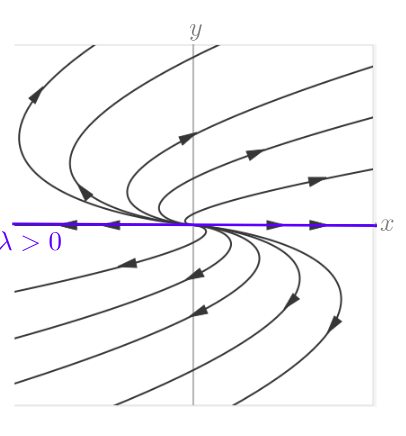
\includegraphics[scale=0.5]{degenerate.png}

This is also attracting or repelling depending on the sign of $\lambda$.


Let's put our results together:


\begin{tabular}{ c c c}
 \textbf{Name} & $\mathbf{\lambda_1, \lambda_2}$  & \textbf{Description} \\
 \hline
 Nodal source/sink & \lambda_1\lambda_2 > 0 & $\lambda_1, \lambda_2$ have same sign \\
 Saddle node & \lambda_1\lambda_2 < 0 & $\lambda_1, \lambda_2$ have different signs\\
 Center & $\lambda_1,\lambda_2 = \pm \mu i$ & $\lambda_1,\lambda_2$ are  purely imaginary \\
 Spiral & $\lambda_1,\lambda_2 =  r \pm \mu i$ & $\lambda_1,\lambda_2$ are complex with a real part \\
 Comb & $\lambda_1 = 0,\lambda_2 \neq 0$ & One $\lambda_1$ is zero while the other is non-zero \\
 Star node & $\lambda_1=\lambda_2$ & Repeated eigenvalue with $\mathbf{P} = \lambda_1\mathbf{I}$
 \\
 Degenerate node & $\lambda_1=\lambda_2$ & Repeated eigenvalue with $\mathbf{P} \neq \lambda_1\mathbf{I}$
\end{tabular}


\subsection{Trace-Determinant Plane}
We know that our 2x2 system looks like
$$
\begin{bmatrix}
    x' \\
    y' \\
\end{bmatrix}
=
\begin{bmatrix}
    p_{11} & p_{12} \\
    p_{21} & p_{22} \\
\end{bmatrix}
\begin{bmatrix}
    x \\
    y \\
\end{bmatrix}
$$

We know that from our previous discussion that the eigenvalues of the matrix $\mathbf{P}$ determine the solution of this system.

The eigenvalues of a matrix can be solved by solving the following equality:

$$\det(\mathbf{P}-\lambda \mathbf{I}) = \mathbf{0}$$

In our case, this is just:

$$
\text{det}\left(
\begin{bmatrix}
    p_{11} - \lambda & p_{12} \\
    p_{21} & p_{22} - \lambda \\
\end{bmatrix}\right) = 0
$$

Using the formula for calculating determinants, we get:

$$( p_{11} - \lambda)(p_{22} - \lambda)- p_{12}p_{21} = 0$$

This simplifies to:

$$\lambda^2 - (p_{11} + p_{22})\lambda + (p_{11}p_{21}- p_{12}p_{21}) = 0$$

Notice that $p_{11} + p_{22}$ is just the trace of the original coefficient matrix $\mathbf{P}$. Also, $p_{11}p_{21}- p_{12}p_{21}$ is just the determinant of the coefficient matrix.

Thus, the eigenvalues of a 2x2 system is just the solutions to the quadratic:

$$\lambda^2-\Tr(\mathbf{P})\lambda + \det(\mathf{\mathbf{P}}) = 0$$

Using the quadratic formula:

$$\lambda = \frac{\Tr(\mathbf{P}) \pm \sqrt{\Tr(\mathbf{P})^2-4\det(\mathbf{P}) }}{2}$$

This means that whether or not the eigenvalues are real, complex, or repeated is determined entirely by the term $\Tr(\mathbf{P})^2-4\det(\mathbf{P})$!

The eigenvalues are real and unique when:

$$\det(\mathbf{P}) < \frac{\Tr(\mathbf{P})^2}{4}$$

They are complex and unique when:

$$\det(\mathbf{P}) < \frac{\Tr(\mathbf{P})^2}{4}$$

They are repeated reals when:

$$\det(\mathbf{P}) = \frac{\Tr(\mathbf{P})^2}{4}$$

We can thereby graph our results on a trace-determinant plane.

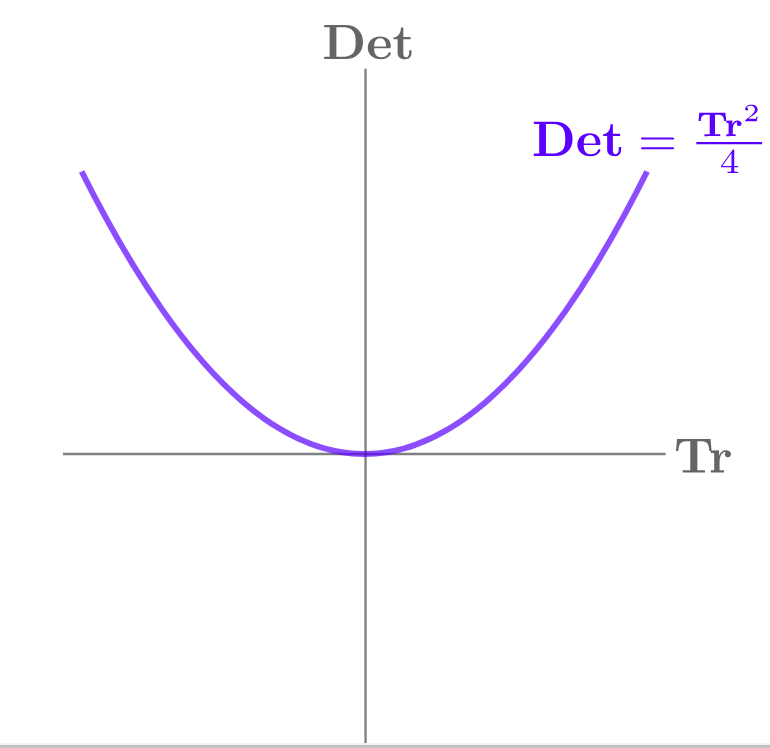
\includegraphics[scale=0.3]{tr-det.png}

If, after we find the trace and determinant of a matrix, it is below the parabola outlined, then we have two unique real roots. If it is on the parabola, we have a repeated root. If it is above the parabola, we have a complex conjugate pair of eigenvalues.


Furthermore, the discriminant of the quadratic expression also tells us the sign of the eigenvalues.

Thus, it is possible to view all the node types on the determinant-trace plane as follows:

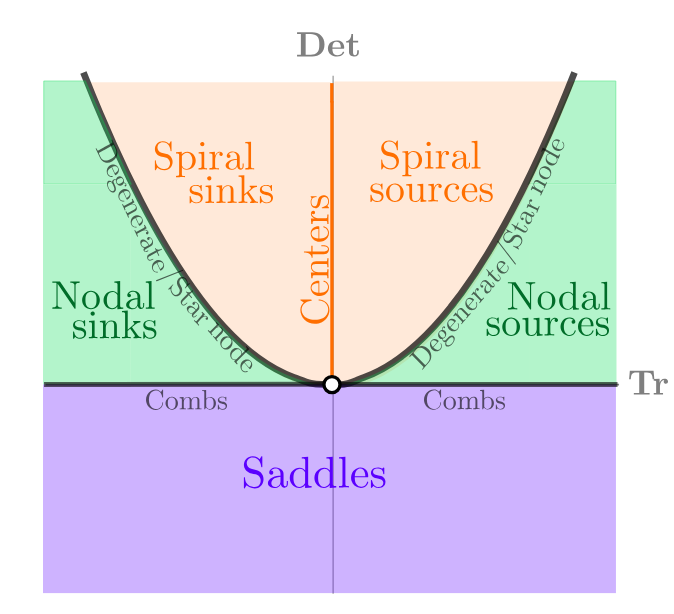
\includegraphics[scale=0.5]{trace_det_full.png}



























\section{Fundamental Matrix and Matrix Exponential}

\section{The Fundamental Matrix}
Say that we've found $n$ solution linearly independent solutions to some system:
$$\mathbf{x'} = \mathbf{Ax}$$


We know from our previous discussion that any solution can in fact be represented as a linear combination of the linearly independent basis solutions:

$$\mathbf{x} = c_1\mathbf{x^{(1)}} + \dots + c_n\mathbf{x^{(n)}}$$

In matrix form this means that any solution is:

Let's consider the matrix formed from the columns of the solutions:


$$
\mathbf{x} =
\begin{bmatrix}
    \vert & & \vert \\
    \mathbf{x}^{(1)} & \dots & \mathbf{x}^{(n)} \\
    \vert & & \vert \\
\end{bmatrix}
\begin{bmatrix}
    c_1 \\
    \vdots \\
    c_n \\
\end{bmatrix}
$$

or 
$$\mathbf{x} = \mathbf{\Psi c}$$

where $\mathbf{\Psi}$ is the \textbf{fundamental matrix} formed by the columns of n linearly independent solutions and $\mathbf{c}$ is the coefficient vector.

How can we find the coefficient vector given some set of initial conditions;

$$\mathbf{x}(t_0) = \mathbf{x^0}$$

Let's use this in the expression above:


$$\mathbf{x}(t_0) = \mathbf{\Psi}(t_0)\mathbf{c} = \mathbf{x^0}$$

We know that that fundamental matrix is inevitable because it is composed of linearly independent vectors. Thus:

$$\mathbf{c} = \mathbf{\Psi}(t_0)^{-1}\mathbf{x^0}$$

And our general solution is given by:

$$\mathbf{x}(t) = \mathbf{\Psi}(t)\mathbf{\Psi}(t_0)^{-1}\mathbf{x^0}$$


If we decide to be clever and pick either a point $t_0$ or another fundamental matrix such that:

$$\mathbf{\Phi}(t_0) = \mathbf{I}$$

Than because $\mathbf{\Phi}(t_0)^{-1} = \mathbf{I}$, our general solution will be:

$$\mathbf{x}(t) = \mathbf{\Phi}(t)\mathbf{x^0}$$

It is possible to always find a $\mathbf{\Phi}$ that satisfies this condition by seeing that:

$$\mathbf{\Phi}(t) = \mathbf{\Psi}(t)\mathbf{\Psi}(t_0)^{-1}$$

Thus:

\begin{mytheo}{Unique Solution to a System}{genSolSys}
    Given a system of homogeneous equations:
    $$\mathbf{x'} = \mathbf{Ax}$$
    with initial conditions:
    $$\mathbf{x}(t_0) = \mathbf{x^0}$$
    
    And given that we have found $n$ linearly independent solutions
    $\mathbf{x^{(1)}}, \dots, \mathbf{x^{(n)}}$  
    
    The unique solution to this differential system of equations is:
    
    $$\mathbf{x}(t) = \mathbf{\Psi}(t)\mathbf{\Psi}(t_0)^{-1}\mathbf{x^0}$$
    
    where:
    $$\mathbf{\Psi}(t)
    =
    \begin{bmatrix}
    \vert & & \vert \\
    \mathbf{x}^{(1)} & \dots & \mathbf{x}^{(n)} \\
    \vert & & \vert \\
    \end{bmatrix}
    $$
\end{mytheo}


\section{Matrix Exponential}
It turns out that it is possible to take exponentials not only of numbers, but of matrices.

What is an exponential? One way to define it is through it's Taylor series:

$$e^{x} = 1 + \sum_{n=1}^\infty \frac{x^n}{n!} = 1 + \frac{x}{1!} + \frac{x^2}{2!} + \dots$$

We can apply this definition with matrices as well. Thus a matrix exponential is defined as:

\begin{mytheo}{Matrix Exponential}{matExp}
    A matrix exponential for a matrix $\mathbf{A}$ is defined as:
    $$e^{\mathbf{A}} = \mathbf{I} + \sum_{n=1}^\infty \frac{\mathbf{A}^n}{n!} = \mathbf{I} + \frac{\mathbf{A}}{1!} + \frac{\mathbf{A}^2}{2!} + \dots$$
\end{mytheo}

It is not too difficult to show \hyperref[sec:prMatExpProp]{(proofs are in the appendix)} that matrix exponentials satisfy some of the properties we are familiar with as exponents:
\label{sec:matExpProp}
\begin{itemize}
    \item Derivative of a matrix exponential:
    $$\dv{e^{\mathbf{A}t}}{t}
    = \mathbf{A}e^{\mathbf{A}t}
    $$
    \item Matrix exponential of a diagonal matrix:
    $$
    \mathbf{D} = 
    \begin{bmatrix}
        d_{1} & & \\
        & \ddots & \\
        & & d_{r} \\
    \end{bmatrix}
    $$
    $$
    e^{\mathbf{D}} = 
    \begin{bmatrix}
        e^{d_{1}} & & \\
        & \ddots & \\
        & & e^{d_{r}} \\
    \end{bmatrix}
    $$
    \item If we have a matrix $\mathbf{A} = \mathbf{S}\mathbf{D}\mathbf{S^{-1}}$
    where $\mathbf{D}$ is a diagonal matrix:
    
    $$e^{\mathbf{\mathbf{S}\mathbf{D}\mathbf{S^{-1}}}} = \mathbf{S} e^{\mathbf{D}}\mathbf{S}^{-1}$$
    
    \item If $\mathbf{AB = BA}$, then $\mathbf{A}e^{\mathbf{B}t} = e^{\mathbf{B}t}\mathbf{A}$
    
    \item  $(e^{\mathbf{A}})^{-1} = e^{-\mathbf{A}}$

    \item If $\mathbf{AB = BA}$, then $e^{\mathbf{A+B}} = e^{\mathbf{A}}e^{\mathbf{B}}$
    
\end{itemize}


From the first property, we can see that the matrix exponential satisfies the properties:

$$(e^{\mathbf{A}t})' = \mathbf{A}e^{\mathbf{A}t}$$

and that at $t=0$:
$$\mathbf{e^{\mathbf{A}*0}} = \mathbf{I}$$


We also know that each column of our fundamental matrix $\mathbf{\Phi}$ is a solution to the differential equation:

$$\mathbf{x}' = \mathbf{Ax}$$

Since each column is a solution, the matrix itself is a solution:

$$\mathbf{\Phi}' = \mathbf{A\Phi}$$

We also know that $\mathbf{\Phi}(t_0) = \mathbf{I}$

If we choose $t_0 = 0$, then we have:

$$\mathbf{\Phi}(0) = \mathbf{I}$$

Thus:
$$\mathbf{e^{\mathbf{A}t}} = \mathbf{\Phi}(t)$$



\begin{mytheo}{Matrix Exponential Solution}{matExpSol}
    Given the system
    $$\mathbf{x'} = \mathbf{Ax}$$
    with initial conditions:
    $$\mathbf{x}(0) = \mathbf{x^0}$$
    
    The solution can be given by:
    $$\mathbf{x}(t) = \mathbf{e^{\mathbf{A}t}}x^0$$
    
    where 
    $$\mathbf{e^{\mathbf{A}t}}= \mathbf{\Psi}(t)\mathbf{\Psi}^{-1}(t_0)$$
    
    and $\mathbf{\Psi}(t)$ is just the fundamental matrix containing $n$ linearly independent solutions as columns.
\end{mytheo}

It is possible to find the matrix exponential directly without computing the fundamental matrix. 

If the matrix $\mathbf{A}$ is \textbf{nilpotent} such that there is a $k$ where $\mathbf{A}^k = \mathbf{0}$, then we can see that the from our definition of matrix exponentials that:

$$e^{\mathbf{A}} = \mathbf{I} + \sum_{n=1}^\infty \frac{\mathbf{A}^n}{n!} = \mathbf{I} + \frac{\mathbf{A}}{1!} + \frac{\mathbf{A}^2}{2!} + \dots + \frac{\mathbf{A}^{k-1}}{(k-1)!} + \frac{\mathbf{A}^k}{k!} + \dots$$
$$e^{\mathbf{A}} = \mathbf{I} + \frac{\mathbf{A}}{1!} + \frac{\mathbf{A}^2}{2!} + \dots + \frac{\mathbf{A}^{k-1}}{(k-1)!} + 0 + 0 + \dots$$
$$e^{\mathbf{A}} = \mathbf{I} + \frac{\mathbf{A}}{1!} + \frac{\mathbf{A}^2}{2!} + \dots + \frac{\mathbf{A}^{k-1}}{(k-1)!}$$

which can be computed directly!

How about matrices that are not necessarily nil-potent? 
We know that if we have $n$ eigenvectors, we can make the following equality:

$$\mathbf{AV} = \mathbf{V\Lambda}$$

where $\mathbf{V}$ is the matrix of eigenvectors and $\mathbf{\Lambda}$ is the matrix formed by putting the corresponding eigenvalue in the diagonals.

If we have $n$ linearly independent eigenvectors, it is possible to take the inverse of $\mathbf{V}$:

Thus, we can represent the matrix $A$ as:

$$\mathbf{A} = \mathbf{V\Lambda V^{-1}}$$

Using one of the properties of matrix exponentials, we see that:

$$e^{\mathbf{A}t} = e^{\mathbf{V\Lambda V^{-1}}t} = \mathbf{V}e^{\mathbf{\Lambda} t}\mathbf{V^{-1}} $$

which gives us a convenient way of solving for the matrix exponential.

\subsection{Repeated Roots and Matrix Exponentials}

Since we know that:

$$\dv{e^{\mathbf{A}t}}{t} = \mathbf{A}e^{\mathbf{A}t}$$. All of the columns must satisfy the homogeneous system:

$$\mathbf{x}' = \mathbf{Ax}$$

We also know that since it is a homogeneous system, any linear combination of solutions is also itself a solution. Thus, for any vector $\mathbf{u}$:

$$\mathbf{x} = e^{\mathbf{A}t}\mathbf{u}$$ 

is in fact a solution to the system above. (We can also see that because of our previous equivalency between the fundamental matrix and the matrix exponential.

We know that:

$$e^{\mathbf{A}t} = e^{(\mathbf{A}-\lambda \mathbf{I} + \lambda\mathbf{I})t}$$

Because $\mathbf{A}(\lambda \mathbf{I}) = (\lambda \mathbf{I})\mathbf{A}$, this is also equivalent to:

$$e^{\mathbf{A}t} = e^{\lambda\mathbf{I}t}e^{(\mathbf{A}-\lambda \mathbf{I} )t}$$

Using properties of taking exponentials of a diagonal matrix, this is just:
$$e^{\lambda t}\mathbf{I}e^{(\mathbf{A}-\lambda \mathbf{I} )t}$$

Since we know that $e^{\mathbf{A}t}\mathbf{u}$ is a solution to the system:

$$\mathbf{x'} = \mathbf{Ax}$$

We know that $\mathbf{x} = e^{\lambda t}e^{(\mathbf{A}-\lambda \mathbf{I} )t}\mathbf{u}$ is a solution
for an arbitrary $\lambda$ and $\mathbf{u}$. Let's take the Taylor expansion of this solution:


$$e^{\lambda t}e^{(\mathbf{A}-\lambda \mathbf{I} )t}\mathbf{u} = e^{\lambda t} \left[ \mathbf{I} + \frac{\mathbf{(A-\lambda \mathbf{I}})t}{1!} + \frac{(\mathbf{A-\lambda \mathbf{I}})^2t^2}{2!} + \dots \right]\mathbf{u} $$

$$= e^{\lambda t} \left[ \mathbf{u} + \frac{\mathbf{(A-\lambda \mathbf{I}})\mathbf{u}t}{1!} + \frac{(\mathbf{A-\lambda \mathbf{I}})^2\mathbf{u}t^2}{2!} + \dots \right]$$

If the matrix $A$ has $n$ unique eigenvalues $\lambda_1, \dots, \lambda_n$, we see that if we plug in $\lambda$ as one of the eigenvalues and $\mathbf{u}$ as an eigenvector, by the properties of eigenvalues we get:

$$(A-\lambda_j \mathbf{I}) \mathbf{u_j} = 0$$
$$(A-\lambda_j \mathbf{I})^2 \mathbf{u_j} = 0$$
$$\vdots$$
$$(A-\lambda_j \mathbf{I})^k \mathbf{u_j} = 0$$

Thus, when we put this into the Taylor expansion of the matrix exponential, almost all of the terms cancel out. If we have $n$ unique eigenvalues, we can use this technique to find $n$ solutions:

$$\mathbf{x^{(1)} = e^{\lambda t}\mathbf{u_1}$$
$$\vdots$$
$$\mathbf{x_n^{(n)}} = e^{\lambda t}\mathbf{u_n}$$

Notice how this is in fact the exact same solutions as we initially used to solve a system of differential equations!

What if we in fact repeated roots $\lambda_i=\lambda_j$

If we set $\mathbf{u_i}$ in the Taylor expansion to be the eigenvector for $\mathbf{\lambda_i}$, we get:

$$\mathbf{x^{(i})}= e^{\lambda_i t} \left[ \mathbf{u_i} + 0 + 0 + \dots \right] =  e^{\lambda_i t}\mathbf{u_i}$$

like before.

However, to find  another linearly independent solution, what if instead of using the corresponding eigenvector to the repeated eigenvalue, we instead used a vector that kept a little bit more of our Taylor expansion.

Remember our expansion:

$$\mathbf{x^{(j)}} = e^{\lambda_i t}e^{(\mathbf{A}-\lambda_i \mathbf{I} )t}\mathbf{u} = e^{\lambda_i t} \left[ \mathbf{u_j} + \frac{\mathbf{(A-\lambda_i \mathbf{I}})\mathbf{u_j}t}{1!} + \frac{(\mathbf{A-\lambda \mathbf{I}})^2\mathbf{u_j}t^2}{2!} + \dots \right]$$

Instead of finding a $\mathbf{u}$ that makes:

$$(A-\lambda_i \mathbf{I}})\mathbf{u_j} = 0$$

let's find a $\mathbf{u_j}$ such that:

$$(A-\lambda \mathbf{I}})\mathbf{u_j} \neq 0$$
and 
$$(A-\lambda \mathbf{I}})^2\mathbf{u_j} = 0$$

The second condition ensures that all the initial terms in the Taylor expansion are in fact 0.


If we can in fact find a vector like this, then we can get another linearly independent solution:


$$\mathbf{x^{(j)}} = e^{\lambda t} \left[ \mathbf{u_j} + \frac{\mathbf{(A-\lambda \mathbf{I}})\mathbf{u_j}t}{1!} + 0 + 0 + \dots \right]$$

It turns out that (not too difficult to prove) that
$\mathbf{(A-\lambda \mathbf{I}})\mathbf{u_j}$ is just our original eigenvector for the eigenvalue $\lambda_i$:

Thus, we have another solution:

$$\mathbf{x^{(j)}} = e^{\lambda t} \left[ \mathbf{u_j} + \mathbf{u_i}t \right]$$

This is the exact same solution as we had before in the case of repeated eigenvalues where $\mathbf{u_j}$ is our generalized eigenvector.

We can extend this further with same logic for repeated eigenvalues of $k = 3,4,\dots$ by just expanding the Taylor expansion one term further each time.


\section{Non-homogeneous Case}
There are three ways we will discuss solving a non-homogeneous differential equation of the form:

$$\mathbf{x' = Px + g}$$


\subsection{Diagonalization}

Say that we try the solution:

$$\mathbf{x = Ty}$$

where $\mathbf{T}$ is an arbitrary constant matrix.

Putting this into our non-homogeneous equation, we see:

$$\mathbf{(Ty)' = PTy + g}$$
$$\mathbf{Ty' = PTy + g}$$

If $\mathbf{T}$ has an inverse:

$$\mathbf{y' = (T^{-1}PT)y + T^{-1}g}$$

If $\mathbf{P}$ has $n$ linearly independent eigenvectors, then we know that:

$$\mathbf{P=S\LambdaS^{-1}}$$

Thus:
$$\mathbf{\Lambda = S^{-1}PS}$$

where $\mathbf{\Lambda}$ is the diagonal matrix of eigenvalues and $\mathbf{S}$ is the matrix of corresponding eigenvectors.

Thus, if we set $\mathbf{T=S}$, we see that we get:

$$\mathbf{y' = \Lambda y + T^{-1}g}$$

Since $\mathbf{\Lambda}$ is a diagonal matrix and $\mathbf{T^{-1}g}$ is just a vector, we see that this is equivalent to solving the first order differential equations:

$$
y_1' = \lambda_1 y_1 + h_1
$$
$$
\vdots
$$
$$
y_n' = \lambda_1 y_n + h_n
$$

where $h_1, \dots, h_n$ are just the components of the vector $\mathbf{T^{-1}g}$

These first order differential equations can be solved using first-order techniques such as the intergrating factors.


\subsection{Undetermined Coefficients}

This method is useful if for the system:
$$\mathbf{x' = Px + g}$$

$\mathbf{P}$ is a constant matrix and $\mathbf{g}$ is the sum of constants, polynomials, exponentials or sinusoidals.

In the case of an exponential non-homogeneous term $Ae^{rt}$, if the solution to the homogeneous solution also has something of the form $e^{rt}$ (this is when $r$ is an eigenvalue of the coefficient matrix), then we must guess the solution:

$$\mathbf{x} = ae^{rt} + bte^{rt}$$

This is slightly different from our discussion in the previous chapter where we only had to guess the solution $te^{rt}$ for a repeated root.

Thus, what we want to do is:
\begin{enumerate}
    \item Break $\mathbf{g(t)}$ into its components (polynomial, exponential, sinusoidal, etc.).
    \item Check if any of the terms that we broke down looks like the homogeneous solution
    \item Guess a solution that is linear combination of the components we found initially. If we see a repeat a homogeneous solution, multiply that by t and add it our trial solution
\end{enumerate}


This is best illustrated by an example:

Say we have the differential equation:

$$\mathbf{x}' = 
\begin{bmatrix}
    -2 & 1 \\
    1 & -2 \\
\end{bmatrix}
\mathbf{x}
+ \begin{bmatrix}
    2e^{-t} \\
    3t
\end{bmatrix}
$$

Let's first break this down into it's the non-homogeneous part into it's components:

$$\mathbf{g} = 
\begin{bmatrix}
    2 \\
    0
\end{bmatrix}
e^{-t}
+ 
\begin{bmatrix}
    0 \\
    3
\end{bmatrix}t$$

If we solve for the homogeneous solution of the matrix $\mathbf{A}$, we see that there is in fact a solution of the form $e^{-t}$. Thus, our trial solution is of the form:

$$\mathbf{x} = \mathbf{a}te^{-t} + \mathbf{b}e^{-t} + \mathbf{c}t + \mathbf{d} $$

which we can plug into our original equation and equate coefficients to solve for $\mathbf{a}, \mathbf{b}, \mathbf{c}, \mathbf{d}$.

\subsection{Variation of Parameters}

This method us very similar to the one described for solving the non-homogeneous differential equation in the n'th order case.

For the system:

$$\mathbf{x' = Ax + g}$$

Let's use some combination of the homogeneous solution to try to find the solution to the non-homogeneous equation.

[Note, that we are not looking for a linear combination of the homogeneous solutions. This would simply evaluate our differential equation to $\mathbf{0 = g}$ which is incorrect].

Since our fundamental matrix consists of solutions to the homogeneous differential equations as columns, we can represent a potential trial solution as:

$$\mathbf{x} = \mathbf{\Psi u}(t)$$

Note that I put $\mathbf{u}(t)$ instead of $\mathbf{u}$ to emphasize that we're looking for non-constant coefficients.

Putting this into our differential equation:

$$(\mathbf{\Psi u}(t))' = \mathbf{A}\mathbf{\Psi u}(t) + \mathbf{g}}$$

Using the product rule,
$$\mathbf{\Psi' u}(t) + \mathbf{\Psi u'}(t)= \mathbf{A}\mathbf{\Psi u}(t) + \mathbf{g}}$$

We also know that:

$$\mathbf{\Psi'} = \mathbf{A\Psi}$$

since the columns of $\mathbf{\Psi}$ are all solutions to the system:

$$\mathbf{x' = Ax}$$

Putting this into our initial equation, we get:

$$\mathbf{A\Psi u}(t) + \mathbf{\Psi u'}(t)= \mathbf{A}\mathbf{\Psi u}(t) + \mathbf{g}}$$

which results in the term $\mathbf{A\Psi u}(t)$ cancelling out on both sides. This gives us:

$$\mathbf{\Psi u'}(t)= \mathbf{g}}$$

Since we know that $\mathbf{\Psi}$ has linearly independent columns, we know that it must in fact be invertible. Therefore:

$$\mathbf{u'}(t)= \mathbf{\Psi^{-1}g}}$$

We can solve for $\mathbf{u'}(t)$ by integrating both sides. 

$$\mathbf{u}(t) = \int{\mathbf{\Psi^{-1}(t)}\mathbf{g}}(t) \dd t + \mathbf{c}$$

where I emphasized the dependence on $t$. The vector $\mathbf{c}$ is just a constant vector to represent the full span of the solution.

Thus, the full set of solutions for $\mathbf{x}$ are:

$$\mathbf{x} = \mathbf{\Psi u}(t) = \mathbf{\Psi}(t)\int{\mathbf{\Psi^{-1}}(t)\mathbf{g}}(t) \dd t + \mathbf{\Psi}(t)\mathbf{c}$$

What if we have an IVP with some initial condition such that:

$$\mathbf{x}(t_0) = \mathbf{x^0}$$

Hmm, the first thing we can do is take advantage of the fact that the anti derivative term above can be represented as a definite integral plus another constant since:

$$\int a(t) \dd t + c = \int_{t_0}^t a(t) \dd t + c_1$$

Thus, we can represent our equation above as:


$$\mathbf{x} = \mathbf{\Psi u}(t) = \mathbf{\Psi}(t)\int{\mathbf{\Psi^{-1}}(t)\mathbf{g}}(t) \dd t + \mathbf{\Psi}(t)\mathbf{c}$$


Thus, we can rewrite the above equation as:


$$\mathbf{x}(t) = \mathbf{\Psi u}(t) = \mathbf{\Psi}(t)\int_{t_0}^{t}{\mathbf{\Psi^{-1}}(t)\mathbf{g}}(t) \dd t + \mathbf{\Psi}(t)\mathbf{c_1}$$

We do this so that the entire anti-derivative term cancels out at $t = t_0$.

If we evaluate the expression at $t_0$:


$$\mathbf{x}(t_0) = \mathbf{\Psi}(t)\int_{t_0}^{t_0}{\mathbf{\Psi^{-1}}(t)\mathbf{g}}(t) \dd t + \mathbf{\Psi}(t)\mathbf{c_1} = \mathbf{0} + \mathbf{\Psi}(t)\mathbf{c_1}$$

Since we know from our IVP that $\mathbf{x}(t_0) = \mathbf{x^0}$,

$$\mathbf{c_1} = \mathbf{\Psi^{-1}}(t)\mathbf{x^0}}$$

Thus:

\begin{mytheo}{Variation of Parameters for System of Differential Equations}
    If we have a non-homogeneous differential equation of the form:
    $$\mathbf{x' = Ax + g}$$
    $$\mathbf{x}(t_0}) = \mathbf{x^0}$$
    And we solve for the corresponding homogeneous solution to get the fundamental matrix $\mathbf{\Psi}$ formed from $n$ linearly independent solutions.
    
    If we try:
    $$\mathbf{x} = \mathbf{\Psi u}(t)$$
    
    as a potential solution, we see that we can always find some $\mathbf{u}$(t) that solve the non-homogeneous problem and give us the closed form solution:
    
    $$
    \mathbf{x}(t) = \mathbf{\Psi}(t)\int_{t_0}^{t}{\mathbf{\Psi^{-1}}(t)\mathbf{g}}(t) \dd t + \mathbf{\Psi}(t)\mathbf{\Psi^{-1}}(t)\mathbf{x^0}}$
    $$
    
    
    
\end{mytheo}





%% Goal: complete on Feb 6
\chapter{Series Solutions}
In this chapter we will discuss solutions to second order linear homogeneous differential equations using power series.


\section{Review of Series}
There are some properties of power series that we will rely on in solving differential equations using series:


\begin{itemize}
    \item A power series is in the form of:
    
    $$\sum_{n=0}^{\infty}a_n(x-x_0)^n$$
    
    A power series is said to \textbf{converge} at a point $x$ when:
    
    $$\lim_{m \to \infty}\sum_{n=0}^{m}a_n(x-x_0)^n$$
    
    exists for $x$. 
    
    Trivially, a power series always converges at $x = x_0$
    
    \item A power series \textbf{converges absolutely} at $x$ if the series:
    
    $$\lim_{m \to \infty}\sum_{n=0}^{m}|a_n(x-x_0)^n|$$
    
    exists for $x$.
    
    If something converges absolutely, then it must also converge. The converse is not always true
    
    \item We can test for the absolute convergence of a power series at some point $x$ using the \textbf{ratio test}. If $a_n \neq 0$:
    
    $$\lim_{n\to \infty} \frac{|a_{n+1}(x-x_0)^{n+1}|}{|a_n(x-x_0)^n|}
    = |x-x_0|\lim_{n\to \infty} \frac{|a_{n+1}|}{|a_n|}$$
    
    If the value above is less than 1, the series \textbf{converges} absolutely:
    
    $$
    \lim_{n\to \infty} \frac{|a_{n+1}(x-x_0)^{n+1}|}{|a_n(x-x_0)^n|} < 1
    $$
    
    If the value is greater than one, than the series \textbf{diverges}:
    
    $$
    \lim_{n\to \infty} \frac{|a_{n+1}(x-x_0)^{n+1}|}{|a_n(x-x_0)^n|} > 1
    $$
    
    If the value is in fact just 1, than the test is inconclusive. 
    
    
    \item If we find that a power series converges at some $x_1$, than the series converges for all $x$ such that $x$ is within $|x_1-x_0|$ from $x_0$
    
    Similarly if we find that a power series diverges at some $x_1$, then it diverges for all $x$ such that x is further than $|x_1-x_0|$ away from $x_0$
    
    
    \item The \textbf{radius of convergence} $\rho$ of a power series is a non-negative number such that the power series converges absolutely for values of $x$ that are less than $\rho$ around $x_0$ in both directions and diverges for values of $x$ further than $\rho$ away from $x_0$.
    
    If the series only converges at $x_0$, then $\rho = 0$. If it converges everywhere, then $\rho = \infty$
    
    At the point $\rho$ away from $x_0$, it is inconclusive whether or not the series converges or not.
    
    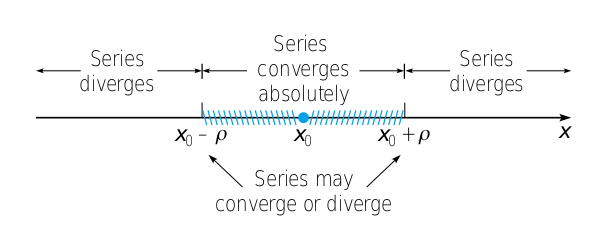
\includegraphics[scale=0.5]{convergence.png}
    
    \item In the following properties we will use two series $a(x) = \sum_{n=0}^{\infty}a_n(x-x_0)^n$ and $b(x) = \sum_{n=0}^{\infty}b_n(x-x_0)^n$
    
    where both $a(x)$ and $b(x)$ converge for some $x$ such that $|x-x_0| < \rho$, $\rho > 0$. We will be considering only values of $x$ in the radius of convergence:
    
    We can add and subtract two series term wise:
    
    $$a(x) \pm b(x) = \sum_{n=0}^{\infty}(a_n \pm b_n)(x-x_0)^n  $$
    
    \item We can multiply two series:
    
    $$
    a(x)b(x)
    = \left[\sum_{n=0}^{\infty}a_n(x-x_0)^n \right] \left[\sum_{n=0}^{\infty}b_n(x-x_0)^n \right]
    = \sum_{n=0}^{\infty}c_n(x-x_0)^n
    $$
    
    where $c_n$ can be formed by collecting coefficients of common exponents $c_n = a_0b_n + \dots + a_nb_0$
    
    If $b(x_0) \neq 0$, i.e.$b_0 \neq 0$ then we can also divide two series:
    
    $$
    \frac{a(x)}{b(x)}
    = 
    \frac{
    \sum_{n=0}^{\infty}a_n(x-x_0)^n }{ \sum_{n=0}^{\infty}b_n(x-x_0)^n}
    = 
    \sum_{n=0}^{\infty}d_n(x-x_0)^n}
    $$
    
    You can find $d_n$ by equating coefficients.
    
    Note: In the case of division, the radius of convergence of the two series may decrease from $\rho$.
    
    \item We can take an infinite amount of derivatives of a power series around our radius of convergence:
    
    $$
    f(x)
    = \sum_{n=0}^{\infty}a_n(x-x_0)^n 
    = a_0 + a_1(x-x_0) + a_2(x-x_0)^2 + \dots
    $$
    $$
    f'(x)
    = a_1 + 2a_2(x-x_0) +
    \dots
    =  \sum_{n=1}^{\infty}na_n(x-x_0)^{n-1}
    $$
    $$
    f''(x)
    = 2a_2 + 6a_3(x-x_0) + 
    \dots
    =  \sum_{n=2}^{\infty}n(n-1)a_n(x-x_0)^{n-2}
    $$
    $$\vdots$$
    
    
    
    
    
    
    
    
    \item The value of $a_n$ can be given by:
    
    $$a_n = \frac{a^{(n)}(x_0)}{n!}$$
    
    where $a^{(n)}(x_0)$ is the $n
    th$ derivative of $x$ evaluated at $x_0$
    
    This is called the \textbf{Taylor Series} about the point $x_0$
    
    \item If we have a function $f(x)$ such that we can create a Taylor expansion about some point $x_0$:
    
    $$f(x) = 
    \sum_{n=0}^{\infty}\frac{f^{(n)}(x_0)}{n!}(x-x_0)^n$$
    
    we call this function $f(x)$ \textbf{analytic} around $x_0$. If $f$ and $g$ are analytic, then $f\pm g$, $fg$ and $\frac{f}{g}$ (where $g(x_0) \neq 0$ are all analytic around $x_0$
    \end{itemize}


Okay, that's enough review, let's start solving some differential equations!

\section{Series solution Ordinary Points}
Say we have the linear homogeneous second order differential equation:

$$P(t)y'' + Q(t)y' + R(t)y = 0$$

We assume here and in the future that the functions $P(t), Q(t), R(t)$ are all continuous.

Let's say that we're trying to solve this differential equation around a neighborhood around a point $t_0$

If $P(t_0) \neq 0$, then we know that there is some interval where $P(t) \neq 0$ since $P(t)$ is assumed to be continuous (no holes). We call the point $t_0$ an ordinary point if this is true.


Thus, within this interval, we can divide by $P(t)$ to get:

$$y'' + p(t)y' + q(t)y = 0$$

where $p(t) = \frac{Q(t)}{P(t)}$ and $q(t) =\frac{R(t)}{P(t)} $


In the case of $P(t_0) = 0$, we cannot just divide by $P(t)$ and use the same method we discuss in this section. We call such a point a \textbf{singular point}. There are ways to solve the differential equation, provided we satisfy some conditions. 


By the Existence and Uniqueness theorem, we know that for initial conditions
$y(t_0) = y^0$ and $y'(t_0) = y^0'$ we should always be able to find a unique solution.

Let's try to find a solution in the form of a power series of the form:

$$y(t) 
= \sum_{n=0}^{\infty}a_n(t-t_0)^n 
= a_0 + a_1(t-t_0) + a_2(t-t_0)^2 + \dots$$

Within the radius of convergence, this is "easy" to divide and manipulate. Thus, we can use this formulation to help solve differential equations.

This is best exemplified by an example:


Let's consider the problem:

$$y'' - ty = 0$$

Since $P(t) = 1$ for all $t$, we know that this every point is ordinary. Thus, let's put in our our series into the differential equation:

$$y(t) 
= \sum_{n=0}^{\infty}a_n(t-t_0)^n $$

$$y''(t) 
= \sum_{n=2}^{\infty}n(n-1)a_n(t-t_0)^{n-2} $$

Putting these into our original differential equation:

$$
\sum_{n=2}^{\infty}n(n-1)a_n(t-t_0)^{n-2}
-t\sum_{n=0}^{\infty}a_n(t-t_0)^n = 0
$$

Let's first try to get both series to be combinations of the same powers.

To do this, for the $y''$ series, let's substitute $k = n-2$. This is equivalent to $n = k+2$


$$
\sum_{k=0}^{\infty}(k+2)(k+1)a_{k+2}(t-t_0)^{k}
-t\sum_{n=0}^{\infty}a_n(t-t_0)^n = 0
$$

Let's consider $t_0 = 0$:
$$
\sum_{k=0}^{\infty}(k+2)(k+1)a_{k+2}t^k
-\sum_{n=0}^{\infty}a_nt^{n+1} = 0
$$

Let's replace the second series by $k = n +1$ or $n = k-1$:

$$
\sum_{k=0}^{\infty}(k+2)(k+1)a_{k+2}t^k
-\sum_{k=1}^{\infty}a_{k-1}}t^{k} = 0
$$

Let's get them to the same starting point so we can add the two series together:

$$
(0+2)(0+1)a_2t^0 +
\sum_{k=1}^{\infty}(k+2)(k+1)a_{k+2}t^k
-\sum_{k=1}^{\infty}a_{k-1}t^{k} = 0
$$
$$
2a_2 +
\sum_{k=1}^{\infty} [(k+2)(k+1)a_{k+2} - a_{k-1}]t^{k} = 0
$$

Since all terms of this equation must be 0 in order to satisfy this equation we have:

$$2a_2 = 0$$
and
$$(k+2)(k+1)a_{k+2} - a_{k-1} = 0$$

The first condition can only be satisfied if $a_2 = 0$. The second condition is satisfied when we have the recurrence relationship:

$$a_{k+2} = \frac{a_{k-1}}{(k+2)(k+1)}$$

In terms of $a_0$, we can find the solutions for $n= 0, 3, 6, 9,\dots$

$$a_3 = \frac{a_0}{3\vdot2}$$

$$a_6 = \frac{a_3}{5\vdot6} = \frac{a_0}{2 \vdot 3 \vdot 5 \vdot 6}$$
$$\vdots$$

This is just:

$$a_{3n} = \frac{a_0}{2 \vdot 3 \vdot 5 \vdot 6 \vdot \dots \vdot (3n-4) \vdot (3n-3) \vdot (3n-1) \vdot (3n)}$$

for $n = 1,2,3, \dots$

Similarly, we can find solutions in terms of $a_1$ for $a_4, a_7, a_10, \dots$:

$$a_{3n + 1} = \frac{a_1}{3 \vdot 4 \vdot 6 \vdot 7 \vdot \dots \vdot (3n-3) \vdot (3n-2) \vdot (3n) \vdot (3n+1)}$$

Since $a_2 = 0$ all values of $a_{3n+2}$ are also 0. Thus $a_5, a_8, a_11, \dots = 0$

Thus, our entire solution can be summarized as:

$$y(t) 
= \sum_{n=0}^{\infty}a_nt^n $$

$$
= a_0\left[ 1 + \frac{t^3}{3\vdot 2} + \frac{t^6}{2\vdot3\vdot 5 \vdot 6}  + \dots + \frac{t^{3n}}{2 \vdot 3 \vdot 5 \vdot 6 \vdot \dots \vdot (3n-4) \vdot (3n-3) \vdot (3n-1) \vdot (3n)} + \dots \right]
$$
$$
+ a_1\left[ 1 + \frac{t^4}{3\vdot 4} + \frac{t^7}{3\vdot4\vdot 6 \vdot 7}  + \dots + \frac{t^{3n+1}}{3 \vdot 4 \vdot 6 \vdot 7 \vdot \dots \vdot (3n-3) \vdot (3n-2) \vdot (3n) \vdot (3n+1)} + \dots \right]
$$
$$
= 
a_0\left[ 1 + \sum_{n=1}^{\infty} \frac{t^{3n}}{2\vdot3\dots(3n-1)\vdot(3n)}\right]
+ a_1\left[ 1 + \sum_{n=1}^{\infty} \frac{t^{3n+1}}{3\vdot4\dots(3n)\vdot(3n+1)}\right]
$$

Thus we have a linear combination of two series. Do the two series converge? We can easily check that yes, for all $x$, both of the series converge. 

We can easily verify that for a point $t_0 = 0$, that the Wronskian formed by the two series and their derivatives is non-zero. Thus, we have found two linearly independent solutions to our differential equation.





\subsection{Justification of Analytic Solutions}
In the past example, we guessed that the answer was going to be in the form of a series solution. However, for an ordinary point, how do we know for sure that the solution is indeed an analytic function?


Say we have the differential equation:


$$P(t)y'' + Q(t)y' + R(t)y = 0$$

and let's consider some interval around $t_0$ such that $P(t_0) \neq 0$:

$$y'' + p(t)y' + q(t)y = 0$$

Say we have a solution of the form:
$$y(t) = \phi = \sum_{n=0}^{\infty}a_n(t-t_0)^n$$

if we can show that it is possible to always find coefficients that satisfy our differential equation in an interval around an ordinary point, we should be done with our proof.

Let's take the m'th derivative of $\phi$:

$$\phi^{(m)}(t) = \sum_{n=m}^{\infty}\frac{n!}{(n-m)!}a_n(t-t_0)^{n-m}$$

When we evaluate this at $t = t_0$, we see that all the terms of the infinite sum become 0 except for when $n=m$:

$$\phi^{(m)}(t_0) = \frac{m!}{(m-m)!}a_m(0)^{0} + 0 + 0 + \dots = m!a_m$$

$$a_m = \frac{\phi^{(m)}}{m!}$$

If we are given the initial conditions $y(t_0) = y^0$ and $y'(t_0) = y^0'$, we can see that this corresponds to:

$$a_0 = \frac{y^0}{0!} = y^0$$
$$a_1 = \frac{y^0'}{1!} = y^0'$$

How do we find the other coefficients?

We know that $\phi$ satisfies our original differential equation:

$$\phi'' + p(t)\phi' + q(t)\phi = 0$$
Rearranging, we see that:

$$\phi'' = - p(t)\phi' - q(t)\phi$$

and thus:

$$a_2 = \frac{- p(t)\phi'(t_0) - q(t)\phi(t_0)}{2!}$$

which we can solve for since we know $\phi(t_0)$ and $\phi'(t_0)$ from our initial conditions.

We can continue our analysis by taking the derivative of our original expression:

$$\phi''' = - p(t)\phi'' - (p'(t) + q(t))\phi' - q'(t)\phi$$

If we evaluate this at $t_0$, we can form an expression for $a_3$ as well.

We can continue this tedious process to compute the coefficients for an arbritrarily large $a_n$. This is not a recommended way of solving a series problem, but it is useful in showing the existence of solutions.

The only thing that is necessary to find $a_n$ for an arbritrarily large $n$ around an ordinary point is just that we can calculate an arbritrarily large derivative for our power series and for $p$ and $q$. 


We can always calculate arbritrarily large derivatives for power series so that should not be a problem. However, it turns out that we need to condition our $p$ and $q$ to also in fact be \textbf{analytic} (have a convergent Taylor Series around $t_0$ in order to guarantee a solution. Note that this is a stronger condition than simply being infinitely differentiable, as one might initially assume (WHY?)

Thus:

$$
p(t) = \sum_{n=0}^{\infty}p_n(t-t_0)^n
$$

$$
q(t) = \sum_{n=0}^{\infty}q_n(t-t_0)^n
$$


Therefore we can establish the following theorem:

\begin{mytheo}{Existence of Power Series Solution}{powSolExist}
    Given a differential equation of the form:
    $$P(t)y'' + Q(t)y' + R(t)y = 0$$
    where $P(t), Q(t), R(t)$ are all continuous functions
    
    If we can find a $t_0$ such that $P(t_0) \neq 0$ (an ordinary point) there is an interval around $t_0$ such that the differential equation simplifies to:
    
    $$y'' + p(t)y' + q(t)y = 0$$

    where $p(t) = Q(t)/P(t)$ and $q(t) = R(t)/Q(t)$.
    
    Furthermore, if both $p(t)$ and $q(t)$ are analytic around $t_0$ (i.e. they have convergent Taylor Expansions) it is possible to find the complete solution of the differential equation in the form of a power series:
    
    $$\phi(t) = \sum_{n=0}^{\infty}a_n(t-t_0)^n = a_0y_1(t) + a_1y_2(t)$$
    
    where $a_0$ and $a_1$ are determined by the initial conditions and $y_1$ and $y_2$ are linearly independent analytic solutions around $t_0$
    
    Furthermore, the radius of convergence of this solution is at least as large as the maximum of the radius of convergence of $p$ and $q$
    
\end{mytheo}



\section{Regular Points and Euler Equation Solutions}

Say we have the differential equation we considered before:

$$P(t)y'' + Q(t)y' + R(t)y = 0$$

If we have points $t$ such that $P(t)$ is 0, it turns out that we cannot use the methods we discussed earlier for finding power series solutions.

This is because the corresponding $p(t)$ and $q(t)$ become unbounded when we approach singular points and thus do not have convergent Taylor series. Thus, we may get bounded or unbounded solutions that may or may not be convergent power series.

However, there is a class of singular points that we will discuss in detail where it is in fact possible to find solutions.

We call these points regular singular points. They are defined as having the property:

\begin{mytheo}{Regular Singular Points}{regSing}
    For the differential equation:
     $$P(t)y'' + Q(t)y' + R(t)y = 0$$
     If the point $x_0$ is a singular point, but both the limits below
     
     $$\lim_{t \to t_0}\frac{Q(t)}{P(t)}(t-t_0)$$
     $$\lim_{t \to t_0}\frac{R(t)}{P(t)}(t-t_0)^2$$
     
     are analytic functions (have convergent Taylor Series around $t_0$)
\end{mytheo}


These conditions will make a lot more sense in our discussion of solutions of Euler Equations:

\subsection{Euler Equations}

Euler Equations are a class of differential equations in the form:

$$t^2y'' + aty' + by = 0$$

We know that at $t_0 = 0$ is a singular point since $t_0^2 = 0$

However, we can also verify that $t_0 = 0$ is a regular singular point since:


$$\lim_{t \to 0}\frac{at}{t^2}t = a$$
$$\lim_{t \to 0}\frac{b}{t^2}t^2 = b$$

which are in fact (constant) analytic functions.


Let's try a solution of the form:

$$y = t^r$$

(The reason we're trying this solutionis because at each derivative $y' = rt^{r-1}$ and $$y'' = r(r-1)t^{r-2}$$ when plugged in will give equal powers of $t$)

When we plug this in, we get:

$$t^2r(r-1)t^{r-2} + at rt^{r-1} + bt^r = 0$$
$$r(r-1)t^r + art^r + bt^r = 0$$
$$[r(r-1) + ar + b]t^r = 0$$

Since we're looking for solutions around $t=0$ and not $t=0$, we can divide both sides by it:

$$F(r) = r^2 + (a-1)r + b = 0$$

This is just a quadratic we can solve for using the quadratic formula:

$$r_1, r_2 = \frac{-(a-1) \pm \sqrt{(a-1)^2-4b}}{2}$$

Thus a root that satisfies this quadratic will make $t^r$ a solution.

We're going to get three cases similar to like we did in the case of our discussion of second order differential equations.

We will only consider the interval $t > 0$ for right now, however, we will extend our results in the end.

\subsubsection{Real Distinct Root}
In this case, we have two solutions: $y_1(t) = t^{r_1}$ and $y_2(t) = t^{r_2}$. If we take the Wronskian of the two solutions, we get $t^{r_1}(r_2t^{r_2-1}) - t^{r_2}(r_1t^{r_1-1}) = (r_2-r_1)t^{r_1+r_2-1}$ which is never 0 for $t > 0$ and $r_2 \neq r_1$.

Thus, our full solution is:

$$y = c_1t^{r_1 t} + c_2t^{r_2 t}$$

\subsection{Repeated Roots}

Let's look at our differential equation again:

$$t^2y'' + aty' + by = 0$$

we know that this simplifies to

$$F(r)t^r = 0$$

for $y = t^r$

If we have $F(r) = (r-r_1)^2$ (a repeated root), we have:

$$(r-r_1)^2t^r = 0$$

Let's derive both sides of this expression using the product rule and the fact that $\pdv{x^r}{r} = x^r\ln x$:

$$2(r-r_1)t^r + (r-r_1)^2t^r\ln t = 0$$

We can see that $r = r_1$ also satisfies this equation as well.

Since we know that our original differential equation is equal to $(r-r_1)^2t^r$ if we plug in our solution, we can also take the derivative of it with respect to $r$:

$$\pdv{}{r} t^2\pdv[2]{y}{t} + a\pdv{y}{t} + by = \pdv{(r-r_1)^2t^r}{r}$$

Using the fact that we can rearrange the order of partial derivatives, we see that the LHS simplifies to:

$$t^2\left(\pdv{y}{r}\right)'' + a\left(\pdv{y}{r}\right)' + b\left(\pdv{y}{r}\right) = 2(r-r_1)t^r + (r-r_1)^2t^r\ln t$$

Putting in $y=t^r$ into the LHS:

$$t^2\left(\pdv{t^r}{r}\right)'' + a\left(\pdv{t^r}{r}\right)' + b\left(\pdv{t^r}{r}\right) = 2(r-r_1)t^r + (r-r_1)^2t^r\ln t$$

which simplifies further to:


$$t^2(t^r\ln t)'' + a(t^r\ln t)' + b(t^r\ln t) = 2(r-r_1)t^r + (r-r_1)^2t^r\ln t$$

At $r=r_1$, we know that the RHS of the equation is 0. Thus:


$$t^2(t^{r_1}\ln t)'' + a(t^{r_1}\ln t)' + b(t^{r_1}\ln t) = 0$$

Looking at the above equality we see that $y_2 = t^{r_1}\ln t$ solves our original differential equation!

Thus, we can form two solutions:

$$y(t) = c_1y_1(t) + c_2y_2(t) = c_1t^{r_1} + c_2t^{r_1}\ln t$$



\subsubsection{Complex Roots}
We know that complex roots always come in conjugate pairs. Thus, let's consider the roots $r_1 = \lambda + i\mu$ and $r_2 = \lambda - i\mu$

We can get complex valued solutions by $y_1 = t^{\lambda + i\mu}$ and $y_2 = t^{\lambda-i\mu}$

We know that $x^a = e^{a\ln{x}}$

Thus,

$$y_1, y_2 = t^{\lambda \pm i\mu} = e^{(\lambda \pm i\mu)\ln t}$$
$$e^{\lambda\ln t}e^{\pm i\mu \ln t} = e^{\lambda\ln t}[\cos(\pm \mu \ln t) + i\sin(\pm \mu \ln t)]$$

Simplifying further, we see that our two solutions are given by:

$$y_1, y_2 = e^{\lambda\ln t}[\cos(\mu \ln t) \pm i\sin( \mu \ln t)]$$

The real and imaginary part of this expression are linear combinations of these two solutions so we can find two real valued solutions by:

$$
y_1 = e^{\lambda\ln t}\cos(\mu \ln t)
$$
and
$$
y_2 = e^{\lambda\ln t}\sin(\mu \ln t)
$$

Using the fact that $e^{\lambda\ln t = t^{\lambda}$, we can get our final solutions as:
$$
y_1 = t^{\lambda}\cos(\mu \ln t)
$$
and
$$
y_2 = t^{\lambda}\sin(\mu \ln t)
$$

\subsection{When t is less than 0}
For the past solutions we have both $t^\lambda$ and $\ln t$. However, when $t < 0$ and $\lambda$ is not an integer, these values are hard to interpret (or in the second case, not even defined).

However, it turns out when we make a substitution in our original Euler equation, we can solve for the case when $t < 0$.

Our original Euler Equation was of the form:

$$t^2y'' + aty' + by = 0$$

where we guessed $y = t^r$

Let's define a new variable $x = -t$ where $t < 0$ and $x > 0$.

We know from the chain rule that:

$$\dv{y}{t} = \dv{y}{x} \dv{x}{t}$$
Since $x = -t$
$$\dv{x}{t} = -1$$
This gives us:
$$\dv{y}{t} = -\dv{y}{x}$$

What is the second derivative with respect to t?

$$\dv[2]{y}{t} = \dv{}{t} \left[\dv{y}{t}\right]= \dv{}{t} \left[-\dv{y}{x}\right] =\dv{}{x} \left[-\dv{y}{x}\right]\dv{x}{t} $$
$$=-\dv[2]{y}{x}\dv{x}{t} = \dv[2]{y}{x}$$


We can put these equalities in our original differential equation to get:


$$t^2\dv[2]{y}{x} + at\left[-\dv[1]{y}{x}\right] + by = 0$$

Putting in $t = -x$ and $t^2 = x^2$ we get:

$$x^2\dv[2]{y}{x} + ax\dv{y}{x} + by = 0$$

where $x > 0$

We see this is exactly the problem we had before except we interchanged $t$ with $x$. Thus, the solutions will be the same as before:

\[
y(x) =
\begin{cases}
    c_1x^{r_1} + c_2x^{r_2} & \text{if real and unique } \\
    c_1x^{r_1} + c_2x^{r_1}\ln{x}  & \text{if real and repeated } \\
    c_1x^\lambda \cos{\mu \ln x} + c_2x^\lambda \sin{\mu \ln x} & \text{if complex } \\
\end{cases}
\]

To get the solutions in terms of $t$, we can simplify replace $x$ with $-t$

Since $|t| = -t$ when $t < 0$ and $|t| = t$ when $t>0$, we can represent our solutions in the most general form if we just use the absolute value of $t$.

\begin{mytheo}{Solutions to Euler Equations}{solEuler}
    Say we have an Euler Equation of the form:
    $$t^2y'' + aty' + by = 0$$
    
    For the regular point $t_0 = 0$, we can find solutions in an interval around $t_0$ if we solve the roots of the polynomial:
    
    $$F(r) = r^2 + (a-1)r + b = 0$$
    
    If we get \textbf{two real and unique} roots, then the full solution is given by:
    
    $$\phi(t) = c_1|t|^{r_1} + c_2|t|^{r_2}$$
    
    If we get \textbf{real repeated} roots, then the full solution is given by:

    $$\phi(t) = c_1|t|^{r_1} + c_2|t|^{r_1}\ln{|t|}$$
    
    If we get \textbf{two complex} roots, then the full solution is given by:
    
    $$\phi(t) = c_1|t|^\lambda \cos{\mu \ln |t|} + c_2|t|^\lambda \sin{\mu \ln |t|}$$
    where $r_1, r_2 = \lambda \pm i\mu$
\end{mytheo}


% Goal Complete by Feb 7
\section{The Method of Frobenius}
Let's consider now the case of a homogeneous linear second order differential equation around a regular point.

Say we have the differential equation:

$$P(t)y'' + Q(t)y' + R(t)y = 0$$

Say we have a singular point $t_0$ such that the following conditions are satisfied (it is a regular point):

$$\lim_{t \to t_0}\frac{Q(t)}{P(t)}(t-t_0)$$

$$\lim_{t \to t_0}\frac{R(t)}{P(t)}(t-t_0)^2$$


Let's multiply both sides of original sides by $t^2$:

$$t^2P(t)y'' + t^2Q(t)y' + t^2R(t)y = 0$$

Since the limits above exist, we can divide both sides by P(t):

$$t^2y'' + t\left[t\frac{Q(t)}{P(t)}\right]y' + \left[t^2\frac{R(t)}{P(t)}\right]y = 0$$

We know that the things in the brackets have convergent analytic functions, so let's replace them with $p(t)$ and $q(t)$:

$$t^2y'' + tp(t)y' + q(t)y = 0$$

Notice that this looks a lot like Euler Equations, except instead of constants we have analytic functions.

Since the coefficients are Euler coefficient times an analytic function, then we should guess a similar solution:

$$y = t^r\sum_{n=0}^\infty a_{n}t^{n} = \sum_{n=0}^\infty a_{n}t^{n+r}$$

When we solve for a solution, there are three things we are looking for:

\begin{enumerate}
	\item The value of $r$
	\item The coefficients $a_n$ via some sort of recurrence relationship
	\item The radius of convergence of the series solution
\end{enumerate}

We will only consider the cases of $t > 0$ for the next examples, but we can get the answers for $t < 0$ by making a substitution of variables like we did before.

Let's try putting in this solution into our original differential equation:

$$y = \sum_{n=0}^\infty a_{n}t^{n+r}$$
$$y' = \sum_{n=0}^\infty (n+r)a_{n}t^{n+r-1}$$
$$y'' = \sum_{n=0}^\infty (n+r)(n+r-1)a_{n}t^{n+r-2}$$

Let's also represent our convergent analytic functions as series:

$$p(t) = \sum_{n=0}^\infty p_{n}t^{n}$$
$$q(t) = \sum_{n=0}^\infty q_{n}t^{n}$$

In addition, let's constrain ourselves to the condition that $a_0 \neq 0$ (since if it was 0, when $t=0$, we would just get the trivial solution)

Substituting all of these into our original equation, we get:

$$t^2\sum_{n=0}^\infty (n+r)(n+r-1)a_{n}t^{n+r-2} 
+
t\left[\sum_{n=0}^\infty p_{n}t^{n}\right]\sum_{n=0}^\infty (n+r)a_{n}t^{n+r-1}
+
\left[ \sum_{n=0}^\infty q_{n}t^{n} \right]\sum_{n=0}^\infty a_{n}t^{n+r}
= 0
$$

This is equivalent to:

$$\sum_{n=0}^\infty (n+r)(n+r-1)a_{n}t^{n+r} 
+
\left[\sum_{n=0}^\infty p_{n}t^{n}\right]\sum_{n=0}^\infty (n+r)a_{n}t^{n+r}
+
\left[ \sum_{n=0}^\infty q_{n}t^{n} \right]\sum_{n=0}^\infty a_{n}t^{n+r}
= 0
$$

Expanding out each series:

$$r(r-1)a_0t^r + (r+1)ra_1t^{r+1} + (r+2)(r+1)a_2t^{r+2} + \dots$$
$$+(p_0+p_1t+p_2t^2 + \dots)[ra_0t^r + (r+1)a_1t^{r+1} + (r+2)a_2t^{r+2} + \dots]$$
$$+ (q_0+q_1t+q_2t^2 + \dots)[a_0t^r+a_1t^{r+1} + a_2t^{r+2} + \dots]$$


Let's order by powers of $t$:

$$[a_0(r)(r-1)+a_0p_0r+a_0q_0]t^r$$
$$+ [a_1(r+1)(r) + a_1p_0(r+1) + a_1q_0 + a_0p_1r+a_0q_1]t^{r+1}$$
$$[a_2(r+2)(r+1) + a_2p_0(r+2) + a_2q_0 + a_1p_1(r+1) + a_1q_1 + a_0p_2r + a_0q_2]t^{r+2}$$
$$\dots = 0$$

Taking out some $a_i$:
$$[a_0[(r)(r-1)+p_0r+q_0]]t^r$$
$$+ [a_1[(r+1)(r) + p_0(r+1) + q_0] + a_0[p_1r+q_1]]t^{r+1}$$
$$[a_2[(r+2)(r+1) + p_0(r+2) + q_0] + a_1[p_1(r+1) + q_1] + a_0[p_2r + q_2]]t^{r+2}$$
$$\dots = 0$$

You might begin to notice a pattern! We can further simplify our analysis by considering a function:

$$F(r) = (r)(r-1) + p_0r + q_0$$

Using this function our equation simplifies considerably:

$$[a_0F(r)]t^r$$
$$+ [a_1F(r+1) + a_0[p_1r+q_1]]t^{r+1}$$
$$[a_2F(r+2) + a_1[p_1(r+1) + q_1] + a_0[p_2r + q_2]]t^{r+2}$$
$$\dots = 0$$

We can simplify this one last time to get:

$$a_0F(r)t^r
+ \sum_{n=0}^\infty \left[ a_nF(r+n) + \sum_{k=0}^\infty p_{n-k}(r+k) + q_{n-k} \right]t^{n+r} = 0
$$

Since all the entire expression is equal to 0, all the coefficients must also be 0. Thus, we have two conditions:

$$F(r) = 0$$
$$\sum_{n=0}^\infty \left[ a_nF(r+n) + \sum_{k=0}^\infty p_{n-k}(r+k) + q_{n-k} \right] = 0$$


The first condition is just solving for the roots of the polynomial 



$$F(r) = (r)(r-1) + p_0r + q_0$ = 0$$


We have seen this many times. We can use a method such as the quadratic equation to find the roots of this equation. The trouble comes when we get a repeated root $r_1$. We will discuss this case in another section.

For the second condition, each term in the sum must be 0. 

Let's first consider the case where $F(r+n)$ is non-zero for every $n$:

If this is indeed the case, then it is possible to solve for every $a_n$ for $n=0,1,2,3 \dots$ by just knowing the value of $r$ and the previous values of $a_0, a_1, \dots, a_{n-1}$.


Let's now consider the case where $F(r+n)$ is zero. Say that when we initially solved $F(r) = 0$ we got two unique roots $r_1$ and $r_2$ where $r_1 < r_2$. Let's also say that $r_1$ and $r_2$ only differ by some integer.

In the case of $r_1$, since we know that $r_1 > r_2$ we also know that for any $n=0,1,2,\dots$ $F(r+n) \neq 0$ (since there are only two roots to the polynomial and we're considering the bigger one). Thus, we can always find the coefficients $a_0, a_1, a_2, \dots, a_n$ for any $n$ we choose. Therefore we are guaranteed a solution of the form:

$$y_1(t) = t^{r_1} \sum_{n=0}^\infty a_n(r_1)t^n$$

(where we emphasized that $a_n$ was calculated using values of the root $r_1$)

However for the smaller root $r_2$, we know that since $r_2$ is an integer away from $r_1$, there exists some $k$ such that $r_2 + l = r_1$. This means that when we try to solve for the coefficients $a_n$, we may have trouble finding $a_l$ since $F(r_2+l) = F(r_1) = 0$. In certain cases, we may still find our solution if  

$$\sum_{k=0}^{l-1}a_k[ p_{n-k}(r+k) + q_{n-k} = 0$$

since in this particular case $a_l$ may be arbitrarily set. 

In the case of $r_1$ and $r_2$ differing by some non-integer (like a fraction), we can always find two solutions by:


$$y_1(t) = t^{r_1} \sum_{n=0}^\infty a_n(r_1)t^n$$
$$y_2(t) = t^{r_2} \sum_{n=0}^\infty a_n(r_2)t^n$$

In the case of complex conjugate roots, we know that there is no $l$ such that $r_1 = r_2 + l$, so we can find complex-valued solutions this way. We can find real valued solutions by just taking the real and imaginary part of our expression like we did before.


Another very important point to note is that the radius of convergence will be at least as large as the distance from the next singular point (if the function is complex, this means the distance in the complex plane). 



\section{Special Cases}
In this section we will discuss finding the series solutions near regular points in the case where there are repeated roots to the indicial equation, or there are roots that differ by some integer $l$. 

\subsubsection{Repeated Roots}
In the case where we have repeated roots, we know that it is possible to factor our our indicial equation in the form:

$$F(r) = r(r-1) + p_0r + q_0 = (r-r_1)^2$$

Say that we plug in our guess for the differential equation and get the result:

$$a_0F(r)t^r
+ \sum_{n=0}^\infty \left[ a_nF(r+n) + \sum_{k=0}^{n-1} a_k[ p_{n-k}(r+k) + q_{n-k}] \right]t^{n+r} = 0
$$

Say we somehow found all the coefficients $a_1, \dots, a_{n-1}$ such that the second part of this expression is 0. We're then left with:

$$a_0F(r)t^r = 0$$

Thus:
$$a_0(r-r_1)^2t^r = 0$$

Since $a_0 \neq 0 $:

$$(r-r_1)^2t^r = 0$$

Let's take the derivative of both sides with respect to $r$:

$$2(r-r_1)t^r + (r-r_1)^2rt^r\ln t = 0$$


Notice that $r=r_1$ satisfies this equation as well.

Since this was our original differential equation with our guess plugged in (and some clever choosing of coefficients $a_1, \dots, a_{n-1}$).

By the fact that for continuous functions we can interchange the way we take the derivatives, this is equivalent to first taking the partial derivative of $y$ with respect to $r$ and then putting that into our differential equation. Thus:


$$L\left[\pdv{y}{r}\right] = 2(r-r_1)t^r + (r-r_1)^2rt^{r-1}$$

which we know that when this expression is evaluated at $r_1$ solves our differential equation!

Thus:

$$L\left[\pdv{y}{r} \Bigg|_{r=r_1}\right] = 0$$

We know that $y$ is:

$$y = t^r\sum_{n=0}^\infty a_n(r)t^n $$

Taking the partial derivative of this expression with respect to $r$ give us (using the chain rule):

$$\pdv{y}{r}(r) = t^r \ln t\sum_{n=0}^\infty a_n(r)t^{n} + t^r\sum_{n=0}^\infty a_n'(r)t^n$$

where $a_n'(r)$ is the (complicated) derivative we can find by our second condition.

We can simplify this by rearranging coefficients:

$$\pdv{y}{r}(r) = \ln t \left( t^r\sum_{n=0}^\infty a_n(r)t^{n}\right)  + t^r\sum_{n=0}^\infty a_n'(r)t^n$$

$$= y_1\ln t  + t^r\sum_{n=0}^\infty a_n'(r)t^n$$

Let's evaluate this at $r=r_1$ 

$$y_2 = \pdv{y}{r} \Bigg|_{r=r_1} = y_1\ln t + t^{r_1}\sum_{n=0}^\infty a_n'(r_1)t^n$$


Since in practice, it is actually difficult to determine a closed form of $a_n'$, we often use the form described above and find the actual coefficients by equating them.

Thus,

\begin{mytheo}{Repeated Roots in Indicial Equation}{repRootIndicial}
	Say we have a second order homogeneous differential equation:
	
	$$t^2y'' + t[tp(t)]y' + t^2q(t)y = 0$$
	
	where $t = 0$ is a singular point.
	
	Furthermore say that $tp(t)$ and $t^2q(t)$ are both analytic functions for some radius of convergence $\rho$.
	
	Say that we solve for the roots and find two identical roots
	
	$$F(r) = r(r-1) + p_0r + q_0 = (r-r_1)^2 = 0$$
	
	The form of the first solution can be given by:
	
	$$y_1(t) = |t|^{r_1}\sum_{n=0}^\infty a_nt^n$$
	
	and the form of the second solution is given by:
	
	$$y_2(t) = y_1(t)\ln|t| + |t|^{r_2}\sum_{n=0}^\infty b_nt^n$$
	
	
	
\end{mytheo}

\subsection{Roots Differing by an Integer}

\begin{mytheo}{Roots Differing By an Integer}{rootInt}
	Say we have a second order homogeneous differential equation:
	
	$$t^2y'' + t[tp(t)]y' + t^2q(t)y = 0$$
	
	where $t = 0$ is a singular point.
	
	Furthermore say that $tp(t)$ and $t^2q(t)$ are both analytic functions for some radius of convergence $\rho$.
	
	Say that we solve for the roots $r_1$ and $r_2$ of the indicial equation:
	
	$$F(r) = r(r-1) + p_0r + q_0 = 0$$
	
	If $r_1 > r_2$ and $r_1$ differ with $r_2$ by an integer $L$, $r_1 = r_2 + L$, the form of the two solutions are given by:
	
	$$y_1(t) = |t|^{r_1}\sum_{n=0}^\infty a_nt^n$$
	
	and 
	
	$$y_2(t) = cy_1(t)\ln|t| + |t|^{r_2}\sum_{n=0}^\infty b_nt^n$$
	
	where $c$ is a constant that may be 0
	
	
\end{mytheo}


\hyperref[sec:prRootInt]{The (lengthy) proof of this is given in the appendix.}

\section{Summary of Series Solution near Regular Point}

Putting all we know together about regular points, we get something called the \textbf{Method of Frobenius}


	Say we have a second order homogeneous differential equation:
	
	$$P(t)y'' + Q(t)y' + R(t)y = 0$$
	
	where:
	
	$$\lim_{t \to t_0} \frac{Q(t)}{P(t)}(t-t_0)
	$$
	$$\lim_{t \to t_0} \frac{R(t)}{P(t)}(t-t_0)^2
	$$
	
	both exist and are analytic functions. In addition $t_0$ is a singular point such that that $P(t_0)$ is 0.
	
	For convenience, let's consider only $t_0 = 0$ (the origin). If we want to consider another $t_0 \neq 0$, we can just substitute another variable $x_0 = t-t_0$, such that the function will be centered at 0.
	
	
	Since the limits of the functions above exists, we can multiply both sides of our differential equation and divide by $P(t)$ to obtain:
	
	$$t^2y'' + t[p(t)]y' + [q(t)]y = 0$$
	
	where $p(t) = tQ(t)/P(t)$ and $q(t) = t^2R(t)/P(t)$
	
	
	By definition, both $p(t)$ and $q(t)$ are analytic functions with some convergent Taylor Series around $0$. Let's consider the minimum of the radius of convergence of both of them $\rho$.
	$$p(t) = \sum_{n=0}^\infty p_nt^n$$
	$$q(t) = \sum_{n=0}^\infty q_nt^n$$
	
	If we solve for the roots of the polynomial, we may get four cases for how the solution will look like
	
	$$F(r) = r(r-1) + p_0r + q_0 = 0$$
	
	\begin{enumerate}
		\item \textbf{Real and Unique Roots}
		
		If we have two real and unique roots $r_1$ and $r_2$, we will get two solutions:
		$$y_1(t) = |t|^{r_2}\sum_{n=0}^\infty a_nt^n$$
		$$y_2(t) = |t|^{r_2}\sum_{n=0}^\infty a_nt^n$$
		
		\item \textbf{Complex and Unique Roots}
		
		If we solve the equation and get some complex conjugate roots $r_1, r_2 = \lambda \pm i\mu$, we can just solve for one complex valued solution, and just take the real and complex parts of it:
		
		$$y_1(t) = \Re{|t|^{r_1}\sum_{n=0}^\infty a_nt^n}$$
		$$y_2(t) = \Im{|t|^{r_1}\sum_{n=0}^\infty a_nt^n}$$
		
		\item \textbf{Identical Roots}
		
		If we solve for the indicial equation and get identical roots $r=r_1=r_2$, the solutions are in the form:
		
		$$y_1(t) = |t|^{r_2}\sum_{n=0}^\infty a_nt^n$$
		$$y_2(t) = y_1(t)\ln|t| + |t|^{r_2}\sum_{n=0}^\infty b_nt^n$$
		
		\item \textbf{Roots Differing by an Integer}
		
		
		If we solve for the indicial equation and get two roots such that $r_1 > r_2$ and that $r_1$ differ with $r_2$ by an integer $L$, $r_1 = r_2 + L$, the form of the two solutions are given by:
		$$y_1(t) = |t|^{r_2}\sum_{n=0}^\infty a_nt^n$$
		$$y_2(t) = cy_1(t)\ln|t| + |t|^{r_2}\sum_{n=0}^\infty b_nt^n$$
		
		where $c$ is a constant that may be 0
		
	\end{enumerate}
	
Each of these solutions are convergent on some radius of convergence at least the size of $\rho$ around $t = 0$


























\section{Bessel's Equation}
In this section we will look at a particular example of a linear homogeneous differential equation that can be solved using the method of Frobenius. This differential equation, the \textbf{Bessel equation} is found throughout physics and mathematics.

The equation is:

$$x^2y'' + xy' + (x^2-v^2)y = 0$$

We will only consider $x>0$ for simplicity. Also, $v$ is an arbitrary constant that we can set.

Notice that this is in the form of a regular singular point at $x=0$, with:
$$
p = 1
$$
and 
$$
q = x^2-v^2
$$

which are both analytic functions. Let's try a Frobenius type solution:

$$y = x^r\sum_{n=0}^\infty a_nx^n = \sum_{n=0}^\infty a_nx^{n+r}$$

$$y' = \sum_{n=0}^\infty a_n(n+r)x^{n+r-1}$$
$$y'' =  \sum_{n=0}^\infty (n+r)(n+r-1)a_nx^{n+r-2}$$

where $a_0 \neq 0$

Putting these into our original equation, we get:

$$
x^2\sum_{n=0}^\infty (n+r)(n+r-1)a_nx^{n+r-2}
+ x\sum_{n=0}^\infty a_n(n+r)x^{n+r-1}
+ (x^2-v^2)\sum_{n=0}^\infty a_nx^{n+r} = 0
$$
Simplifying,
$$
= \sum_{n=0}^\infty a_n[(n+r)(n+r-1) + (n+r)]x^{n+r}
+ \sum_{n=0}^\infty a_nx^{n+r+2} -v^2\sum_{n=0}^\infty a_nx^{n+r} = 0
$$ 

We can simplify the middle sum:

$$\sum_{n=0}^\infty a_nx^{n+r+2} = \sum_{n=2}^\infty a_{n-2}x^{n+r}$$

and 
$$(n+r)(n+r-1) + (n+r) = (n+r)^2$$

to get:

$$
= \sum_{n=0}^\infty a_n[(n+r)^2-v^2]x^{n+r}
+ \sum_{n=2}^\infty a_{n-2}x^{n+r}  = 0
$$

Let's put the two summations together by expanding out the first two terms:

$$a_0[(0+r)^2-v^2]x^r + a_1[(1+r)^2-v^2]x^{r+1}
+ \sum_{n=2}^\infty [a_n((n+r)^2-v^2)+a_{n-2}]x^{n+r}$$

$$\boxed{
a_0(r^2-v^2)x^r + a_1[(1+r)^2-v^2]x^{r+1} +  \sum_{n=2}^\infty [a_n((n+r)^2-v^2)+a_{n-2}]x^{n+r}
=0} $$

Since each coefficient of $x$ must be 0, we have three conditions:

\begin{enumerate}
	\item $$a_0(r^2-v^2) = 0$$
	\item $$a_1[(1+r)^2-v^2] = 0$$
	\item $$a_n((n+r)^2-v^2)+a_{n-2} = 0$$
\end{enumerate}

Since $a_0 \neq 0$:

$$r^2 - v^2 = 0$$
$$\boxed{r = \pm v}$$

For the second equation, we see that $r = v$ does not make the part in brackets 0. However, since we can arbitrarily set the coefficients, we can choose to set $a_1 = 0$.

Finally, the third expression gives us a recurrence relationship of finding coefficients based on previous values.


Let's first consider the larger value of the roots $r= +v$.

In this case, we get the recurrence relationship:

$$a_n((n+v)^2-v^2)+a_{n-2} = 0$$

We can simplify the expression in the middle using the identity $a^2-b^2 = (a+b)(a-b)$:

$$a_n(n(n+2v))+a_{n-2} = 0$$

Since for any value of $n$, $n(n+2v)$ never equals 0, we can always find an expression for $a_n$ in terms of $a_{n-2}$:


$$a_n=\frac{-a_{n-2}}{n(n+2v)}$$

Since we set $a_1 = 0$, this means that all odd $a_n$ are also 0 due to this recurrence relationship:

$$a_1=a_3=a_5=\dots=0$$

Thus, we can rewrite our recurrence relationship with $n=2m$ for $m=1,2,3,\dots$:

$$a_{2m}=\frac{-a_{2m-2}}{2m(2m+2v)}
= \frac{-a_{2m-2}}{2^2m(m+v)}$$

Thus,
$$a_2 = \frac{-a_{0}}{2^2\vdot1\vdot(v+1)}$$
$$a_4 = \frac{-a_{2}}{2^2\vdot2\vdot(v+2)} = \frac{a_0}{(2^2)^2\vdot2\vdot(v+2)\vdot(v+1)}$$
$$a_6 = \frac{-a_{6}}{2^2\vdot1\vdot3\vdot(v+3)} = \frac{-a_0}{(2^2)^3\vdot3\vdot2\vdot1\vdot(v+3)\vdot(v+2)\vdot(v+1)}$$

We can continue this pattern to see that:

$$a_{2m}=\frac{(-1)^ma_0}{2^{2m}\vdot m! \vdot(v+m)\vdot\dots\vdot(v+2)\vdot(v+1)} $$


Thus, one solution is always given by:


$$\boxed{
	y_1(x) = \sum_{m=0}^\infty \frac{(-1)^ma_0}{2^{2m}\vdot m! \vdot(v+m)\vdot\dots\vdot(v+2)\vdot(v+1)} x^{n+v}
}$$

What about the other root $r = -v$?

Let's have a look at the recurrence relationship again:

$$a_n((n+r)^2-v^2)+a_{n-2} = 0$$

when $r=-v$, making the same simplification we made earlier:


$$a_n[n(n-2v)]+a_{n-2} = 0$$

Hmm, if the term $n-2v$ equals 0 the recurrence relationship would not be satisfied for $a_{n-2} \neq 0$ and we would have to find another form for the solution.

Thus, we need to be wary of the case:

$$n = 2v$$

or 

$$v = \frac{n}{2}$$

when $v$ is a discrete multiple of $1/2$.

Let's consider the case where $n$ is odd, i.e. $v = 1/2, 3/2, 5/2, \dots$. 

We know that $a_1$ is 0. However, we can also set all of $a_1=a_3=a_5=\dots=0$, so that we wouldn't have to deal with the case of finding $a_n$ when $n$ is odd and $v = n/2$.

In other words, when we're trying to find $a_n$ where $n=2v$, our recurrence relationship will look like:

$$a_n[2v(2v-2v)]+0 = 0$$

which will always be satisfied!

Thus, we only have to worry about cases where

$$v=\frac{n}{2}$$

where $n$ is even, or where:

$$v=m$$
where m is a whole number.

In the case of non-whole number, we can do the exact same thing we did before to find our first solution, except replace $v$ with $-v$

In the case of a whole number, we will have to look at the form of the solution specified by the \hyperref[sec:methodOfFrobenius]{Method of Frobenius}, plug it in and find the coefficients in order to find the second solution.

Thus,

\begin{mytheo}{Bessel's Equations}{bessel}
	For a differential equation of the form:
	$$x^2y'' + xy' + (x^2-v^2)y = 0$$
	
	where $v$ is an arbitrarily constant.
	
	For $x>0$, we can always find one solution by:
	$$
	y_1(x) = \sum_{m=0}^\infty \frac{(-1)^ma_0}{2^{2m}\vdot m! \vdot(v+m)\vdot\dots\vdot(v+2)\vdot(v+1)} x^{n+v}
	$$
	
	For non-whole numbers, we can also find the second linearly independent solution by:
	
	$$
	y_2(x) = \sum_{m=0}^\infty \frac{(-1)^ma_0}{2^{2m}\vdot m! \vdot(-v+m)\vdot\dots\vdot(-v+2)\vdot(-v+1)} x^{n-v}
	$$
	
	The solution in the cases where $v$ is a whole number are more complicated and can be found by trying the form of solution specified in the \hyperref[sec:methodOfFrobenius]{section} above.
	
\end{mytheo}

Bessel equations have far more interesting properties and applications then presented here.

[TODO: gamma functions, solve $v=0$, etc.]


\chapter{Laplace Transform}

\chapter{Partial Differential Equations and Fourier Transform}

\chapter{Boundary Value Problems}

\chapter{First-order case}

\chapter{Questions}
\begin{itemize}
    \item Why does an nth order linear equation with n initial conditions need n linearly independent solutions to fully describe the solution space?
    \item Proof of Uniqueness and Existence theorem (or at least intuition)?
    \item What is Bessels equation?
    \item Is there a form of Abel's equation in higher than 2 dimensions?
    \item Why does putting $t, t^2, \dots $ before solution to a constant coefficient differential homogeneous give us another linearly independent solution for any degree?
    \item Why is a generalized eigenvector guaranteed to exist if we have a eigenvalue with multiplicity greater than one.
    \item In systems of equations, to solve for the non-homogeneous case using undetermined coefficient, why do we have both $te^{\lambda t} + e^{\lambda t}$ as solutions instead of just $te^{\lambda t}$
\end{itemize}

\chapter{Proofs}
\section{\hyperref[th:wronLinInd]{Proof of Wronskian implying linear independence}}
\label{sec:prWronLinInd}
Consider the equation 
$$c_1\bm{f(t)} + c_2\bm{g(t)} = 0$$ 
for some interval $t \in I$. 

We know that is we can find non-zero $c_1$ and $c_2$ such that this equation is always true, the functions $\bm{f(t)}$ and $\bm{g(t)}$ are linearly dependent. On the other hand, if we can find some $t_0 \in I$ such that the only way we can satisfy this equation is by setting $c_1 = c_2 = 0$, then the functions are linearly independent.

Say that the functions have their derivatives defined. Thus, we have a set of equations:
$$c_1\bm{f(t)} + c_2\bm{g(t)} = 0$$ 
$$c_1\bm{f'(t)} + c_2\bm{g'(t)} = 0$$ 

In matrix form:
$$
\begin{bmatrix}
    \bm{f(t)} & \bm{g(t)} \\
    \bm{f'(t)} & \bm{g'(t)} \\
\end{bmatrix}
\begin{bmatrix}
    c_1 \\
    c_2 \\
\end{bmatrix}
=
\begin{bmatrix}
    0 \\
    0 \\
\end{bmatrix}
$$

If the determinant of the matrix (which is the Wronskian) is non-zero for some $t_0 \in I$, we know from basic linear algebra, that the only $\begin{bmatrix}
    c_1 \\
    c_2 \\
\end{bmatrix}$ that satisfies the equation is $\begin{bmatrix}
    0 \\
    0 \\
\end{bmatrix}$ (there is no non-zero null space for the matrix).

Thus, when the \textbf{Wronskian} is non-zero for some $t_0$, the functions must be linearly independent since it is impossible to find a non-zero $c_1$ and $c_2$ that satisfy:
$$c_1\bm{f(t_0)} + c_2\bm{g(t_0)} = 0$$
$$c_1\bm{f'(t_0)} + c_2\bm{g'(t_0)} = 0$$.






\section{\hyperref[th:abel_thm]{Proof of Abel's Theorem}}
\label{sec:abel}
Say we have the differential equation.
$$y''(t) + p_1(t)y'(t) + p_0(t)y(t) = 0$$
Say we also have two solutions $y_1(t)$ and $y_2(t)$ that satisfy this equation:
$$y_1''(t) + p_1(t)y_1'(t) + p_0(t)y_1(t) = 0$$
$$y_2''(t) + p_1(t)y_2'(t) + p_0(t)y_2(t) = 0$$

Let's multiply the top equation by $y_2(t)$ and the bottom equation by $y_1(t)$ and subtract to get rid of the term with $p_0(t)$:

$$y_1''(t)y_2(t) + p_1(t)y_1'(t)y_2(t) + p_0(t)y_1(t)y_2(t) = 0$$
$$y_2''(t)y_1(t) + p_1(t)y_2'(t)y_1(t) + p_0(t)y_2(t)y_1(t) = 0$$

Subtracting yields:
$$y_1''(t)y_2(t) + p_1(t)y_1'(t)y_2(t) - (y_2''(t)y_1(t) + p_1(t)y_2'(t)y_1(t)) = 0$$
which after rearranging and simplifying yields:
\begin{equation}
\label{abel_eq}
(y_1''(t)y_2(t)-y_2''(t)y_1(t))+p_1(t)(y_1'(t)y_2(t)-y_2'(t)y_1(t)) = 0
\end{equation}

multiplying by $-1$ and simplifying some more:
$$(y_1(t)y_2''(t)-y_2(t)y_1''(t))+p_1(t)(y_1(t)y_2'(t)-y_2(t)y_1'(t)) = 0$$
The term $y_1(t)y_2'(t)-y_2(t)y_1'(t)$ looks familiar. In fact, it is the Wronskian of $y_1(t)$ and $y_2(t)$:
$$
    W(y_1(t), y_2(t))(t) =
    \text{det}\left(\begin{bmatrix}
        y_1(t) & y_2(t) \\
        y_1'(t) & y_2'(t) \\
        \end{bmatrix}\right)
    = y_1(t)y_2'(t)-y_2(t)y_1'(t)
$$
It also turns out that (by the chain rule):
$$
W'(y_1(t), y_2(t))(t) = y_1'(t)y_2'(t)-y_2(t)y_1''(t)+y_1(t)y_2''(t)-y_2'(t)y_1'(t)
$$
$$=y_1(t)y_2''(t)-y_2(t)y_1''(t)$$

Returning to equation \ref{abel_eq}, we can substitute in the Wronskian and the derivative to get:
$$W'(y_1(t),y_2(t))(t) + p_1(t)W(y_1(t), y_2(t))(t) = 0$$

This is a separable first order equation for $W(t)$. Thus,

$$\frac{W'(y_1(t),y_2(t))(t)}{W(y_1(t), y_2(t))(t)} = -p_1(t)$$
Integrating both sides and simplifying:
$$\int{\frac{dW}{W(y_1(t), y_2(t))(t)} }= \int{-p_1(t)dt}$$
$$=\ln|W(y_1(t), y_2(t))(t)| = \int{-p_1(t)dt} + c$$
$$W(y_1(t), y_2(t))(t)| = \exp{\left[\int{-p_1(t)dt} + c\right]}$$
$$=c\exp{\left[-\int{p_1(t)dt}\right]}$$


\section{\hyperref[th:WrLinDep]{Proof of Wronskian and Linear Dependence Relationship}}
\label{sec:PrWrLinDep}
This theorem says two main things:
\begin{enumerate}
    
    \item$W(y_1(t), y_2(t))(t) = 0 \implies \text{Linear Dependence}$
    
    \item$ \text{Linear Dependence} \implies W(y_1(t), y_2(t))(t) = 0$
\end{enumerate}
We know that the second statement is true from \hyperref[th:wronLinDep]{this theorem.} The challenge in this proof is to prove the first statement.

Let our two solutions be $y_1(t)$ and $y_2(t)$. Say we have the equation:
$$c_1y_1(t) +c_2y_2(t) = 0$$
The constants $c_1$ and $c_2$ can be zero or non-zero to satisfy this equation. If we can find a $c_1$ and $c_2$ such that they are both non-zero and it always satisfies this solution for any $t$ in some interval $I$, then $y_1(t)$ and $y_2(t)$ are linearly dependent.

From our equation we can take derivatives of both sides to get:
$$c_1y_1(t) +c_2y_2(t) = 0$$
$$c_1y_1'(t) +c_2y_2'(t) = 0$$

Which forms the linear equations:
$$
\begin{bmatrix}
    y_1(t) & y_2(t) \\
    y_1'(t) & y_2'(t) \\
\end{bmatrix}
\begin{bmatrix}
    c_1 \\
    c_2 \\
\end{bmatrix}
=
\begin{bmatrix}
    0 \\
    0 \\
\end{bmatrix}
$$

This equation will be satisfied for some $c_1$ and $c_2$ if and only if the determinant of the matrix is 0. That is when:
$$
\text{det}\left(\begin{bmatrix}
        y_1(t) & y_2(t) \\
        y_1'(t) & y_2'(t) \\
        \end{bmatrix}\right)
$$
which is just the Wronskian.

We might think that completes our proof, however, this is not the case. We've proven that we can always find a non-zero $c_1$ and $c_2$, however, they may not be the \textbf{same} $c_1$ and $c_2$ throughout the equation. 

For example, in the case of the functions $t^3$ and $|t|t^2$ we can in fact find a $c_1$ and $c_2$ such that we always satisfy $c_1t^3+c_2|t|t^2=0$ for any t. However, for $t < 0$, $c_1=c_2=1$ satisfies this equation. In the case of $t>0$, $c_1=-c_1$ will satisfy this equation. Therefore these equations are not linearly dependant even though their Wronskian will be 0 everywhere.

So in order to complete our proof, we need to make use of an additional fact, that $y_1(t)$ and $y_2(t)$ are solutions of a differential equation. 

Say that for the differential equation $y_1(t)$ and $y_2(t)$ are the solution to we have the following arbitrarily initial values on the complete solution $\phi(t)$
$$\phi(t_0) = 0$$
$$\phi'(t_0) = 0$$


We also know that $y_1(t)$ and $y_2(t)$ satisfy this differential equation (by definition) and by superposition, any linear combination of them must also satisfy this equation. Thus, let us consider a possible  general solution to be:

$$\phi(t) = c_1y_1(t) +c_2y_2(t)$$

Using the initial constraints,

$$\phi(t_0) = c_1y_1(t_0) +c_2y_2(t_0) = 0$$
$$\phi'(t_0) = c_1y_1'(t_0) +c_2y_2'(t_0) = 0$$

which solves the matrix equation that we had earlier:
$$
\begin{bmatrix}
    y_1(t_0) & y_2(t_0) \\
    y_1'(t_0) & y_2'(t_0) \\
\end{bmatrix}
\begin{bmatrix}
    c_1 \\
    c_2 \\
\end{bmatrix}
=
\begin{bmatrix}
    0 \\
    0 \\
\end{bmatrix}
$$

If the Wronskian is 0, we can always find $c_1$ and $c_2$ that are both non-zero satisfying this equation (a fact we established earlier). 

Therefore, $\phi(t) = c_1y_1(t) + c_2y_2(t)$ is a solution the differential equation with the initial constraints $\phi(t_0) = 0$ and $\phi'(t_0) = 0$. if the Wronskian of $y_1(t)$ and $y_2(t)$ is zero. 

Another interesting fact is that the trivial solution $\phi(t) = 0$ also satisfies our initial constraints $\phi(t_0) = 0$ and $\phi'(t_0) = 0$.

By the  \hyperref[th:Ex&Un]{Existence and Uniqueness theorem}, if we find one solution satisfying the initial value problem, it must be the only solution the differential equation. Since we found two solutions to the differential equation we're considering, they must be equal to each other for all $t \in I$.
Thus,
$$\phi(t) = c_1y_1(t) +c_2y_2(t) = 0$$
for all $t \in I$

Taking derivatives of both sides and putting into matrix form, we see that:

$$
\begin{bmatrix}
    y_1(t) & y_2(t) \\
    y_1'(t) & y_2'(t) \\
\end{bmatrix}
\begin{bmatrix}
    c_1 \\
    c_2 \\
\end{bmatrix}
=
\begin{bmatrix}
    0 \\
    0 \\
\end{bmatrix}
$$

for $c_1, c_2 \neq 0$, $t \in I$

Thus, when the Wronskian is 0 for two solutions of a second order linear homogeneous differential equation, we can find a universal $c_1$ and $c_2$ that are both non-zero such that $c_1y_1(t) +c_2y_2(t) = 0$ is always satisfied. 


\section{\hyperref[th:expLinInd]{Proof of Linear Independence of exponentials of different degrees}}
\label{sec:prExpLinInd}
We know that  if we show that the Wronskian of two functions $y_1(t)$ and $y_2(t)$ is non-zero at any point, \hyperref[th:wronLinInd]{the functions must be linearly independent.}

Thus, if we show that the Wronskian of $e^{r_1t}$ and $e^{r_2t}$ is 0 for $r_1 \neq r_2$ then they must be linearly independent.

Let's do a proof by contradiction. Suppose that the $r_1 \neq r_2$, but the Wronskian is 0.Thus,

$$
    \text{det}\left(\begin{bmatrix}
        e^{r_1t} & e^{r_2t} \\
        r_1 e^{r_1t} & r_2 e^{r_2t} \\
    \end{bmatrix}\right)
    = 0
$$
Thus,by the definition of a determinant,
$$r_2e^{r_2t}e^{r_1t} -r_1e^{r_1t}e^{r_2t} = 0$$
which simplifies to:
$$(r_2-r_1)e^{(r_1+r_2)t} = 0$$
Since $e^{(r_1+r_2)t} \neq 0$, we can divide both sides by it and get:
$$r_2 -r_1 = 0$$
$$r_2 = r_1$$

which contradicts our assumption that $r_1 \neq r_2$

Thus, the Wronskian is in fact non-zero and the functions $e^{r_1t}$ and $e^{r_2t}$ are linearly independent.

\section{\hyperref[sinLin]{Proof that sine and cosine are linearly independent}}
\label{sec:prSinLin}
If we can show that Wronskian of sine and cosine is non-zero at any particular $t_0$, then the functions are linearly independent.

Let's take the Wronskian of $y_1(t) = \sin(bt)$ and $y_2(t) = \cos(bt)$

$$
    \text{det}\left(\begin{bmatrix}
        \sin(bt) & b\cos(bt)\\
        b\cos{bt} & -b\sin(bt) \\
    \end{bmatrix}\right)
$$
$$=-b\sin^2(bt)-b\sin^2(bt)$$
$$=-b(\sin^2(bt) + \cos^2(bt)$$
By the elementary trig identity $\sin^2(bt) + \cos^2(bt) = 1$, we get:
$$W(\sin(bt),\cos(bt))(t)=-b$$
which is non-zero everywhere when $b$ is non-zero.

Because, the Wronskian indeed is 0 everywhere, the functions $\sin(bt)$ and $\cos(bt)$ are linearly independent


\section{\hyperref[repRoot]{Proof of finding Linearly Independent solutions for repeated roots (2nd Order)}}
\label{sec:PrRepRoot}
Say that we have a homogeneous linear differential equation of 2nd order with constant coefficients:

$$y''(t) + a_1y'(t) + a_0y = 0$$

Say that we solve for the characteristic polynomial and get an expression in the form of:

$$r^2 + a_1r + a_0 = 0$$

Furthermore, say that when we solve this polynomial (for example, using the quadratic equation), we get two repeated roots $r_1=r_2$.

We need to find another linearly independent solution if we wish to span the complete solution space.

We know that $y(t) = Ce^{r_1t}$ must be a solution (since it always satisfies the equation. Let's see if we can multiply it by a function $u(t)$ and see if the complete function satisfies our original differential equation.

Thus, another potential solution is:

$$y_2(t) = u(t)e^{rt}$$

Plugging that in gives us:
$$(u(t)e^{rt})'' + a_1(u(t)e^{rt})' + a_0(u(t)e^{rt}) = 0$$

Applying the chain rule gives us:
$$(u''(t)e^{rt}+2u'(t)(re^{rt}) + u(t)(r^2e^{rt})) + a_1(u'(t)e^{rt} + u(t)(re^{rt}))' + a_0(u(t)e^{rt}) = 0$$
Collecting terms:
$$u(t)e^{rt}(r^2+a_1r+a_0) +u''(t)e^{rt} + 2u'(t)(re^{rt}) + a_1 u(t)(re^{rt}) = 0$$
Since we know $r$ satisfies the characteristic polynomial equation, $(r^2+a_1r+a_0)$ must be 0. Thus,
$$u''(t)e^{rt} + 2u'(t)(re^{rt}) + a_1 u(t)(re^{rt}) = 0$$
Simplifying by dividing by $e^{rt}$ (which is never 0) yields,
$$u''(t) + u'(t)(2r+a_1) = 0$$

Hmm, what should we do now?

We know that the roots of a quadratic in the form $x^2 + bx + c = 0$ are given by the quadratic formula:
$$r = \frac{-b \pm \sqrt{b^2-4c}}{2}$$
When we have repeated roots, the discriminant $b^2-4ac$ is 0, giving us:
$$r = \frac{-b}{2}$$


Putting this in our equation yields:
$$u''(t)+u'(t)(2r+a_1) = 0$$
$$u''(t)+u'(t)(2(\frac{-a_1}{2}+a_1) = 0$$
$$u''(t) + u'(t)(-a_1+a_1) = 0$$
$$u''(t) = 0$$

Integrating we get:
$$u'(t) = c$$
$$u(t) = ct + d$$

Plugging back into original equation, we get:
$$y_2(t) = (ct+d)e^{rt}$$

We can remove the $de^{rt}$ part, since that is already a linear multiple of our first solution.

Is the equation, $y_2(t) = te^{rt}$ linearly independent with $y_1(t) = e^{rt}$

We can take the Wronskian and see if it is non-zero at any point in the interval we're considering:


$$
    \text{det}\left(\begin{bmatrix}
        e^{rt} & te^{rt}\\
        re^{rt} & rte^{rt}+ te^{rt} \\
    \end{bmatrix}\right)
$$
$$
    = e^{rt}(rte^{rt}+te^{rt}) - te^{rt}re^{rt}
    = (e^{rt})^2(rt+t-rt)
    = te^{rt}
$$
which is in fact non-zero everywhere where $t$ is non-zero!

\section{\hyperref[th:sinPlusCosin]{Proof of Ssum of Sine and Cosine of same frequency}}
\label{sec:prSinPlusCosin}
First proof:

Consider taking the dot product between two vectors $(a,b)$ and a vector arbritrarily defined on the unit circle $(\cos(\theta),\sin(\theta))$

$$(a,b)\cdot(\cos(\theta),\sin(\theta)) = a\cos(\theta) + b\sin(\theta)$$

We know that by the geometric interpretation of the dot product, that:

$$(a,b)\cdot(c,d) = \lVert(a,b)\rVert*\lVert(c,d)\rVert*\cos(\text{angle b/w vectors})$$

Thus, the dot product of $(a,b)$ and $(\cos(\omega t),\sin(\omega t))$ is just:

$$(a,b)\cdot(\cos(\theta),\sin(\theta)) = \lVert(a,b)\rVert*\lVert(\cos(\theta),\sin(\theta)\rVert*\cos(\text{angle b/w vectors})$$

We know that $\lvert(\cos(\theta),\sin(\theta))\rvert =1$ so this simplifies to 

$$\lVert(a,b)\rVert*\cos(\text{angle b/w vectors})$$

The magnitude of $(a,b)$ is simply $\sqrt{a^2+b^2}$

The angle between both vectors is just going to be the difference between the angle created by the vector $(a,b)$ and $\theta$. 

Using basic trigonometry, the angle of the vector $(a,b)$ is $\phi = \tan^{-1}(b/a)$

Thus we get:

$$(a,b)\cdot(\cos(\theta),\sin(\theta) = A\cos(\theta - \phi)$$

where
$$A = \sqrt{a^2+b^2}$$
$$\phi = \tan^{-1}(b/a)$$

Since both interpretations of the dot product yield the same result, we get:

$$a\cos(\theta) + b\sin(\theta) = A\cos(\theta - \phi)$$

[INSERT PICTURE]

Second proof:

It turns out that

$$a\cos(\theta) + b\sin(\theta) = \Re{(a-bi)*(\cos(\theta) + i\sin(\theta)}$$

(you can quickly verify this!)

We know that the expression $a-bi$ like all complex numbers, can be represented in the form $Ae^{i\phi}$

In this case $A$ is the magnitude of the complex number, which is just $\sqrt{a^2+b^2}$.

In addition, $\phi$ is the angle formed by the real and imaginary part of the complex number. This will be negative since there is a negative imaginary part in the expression we're considering. In this case the angle between these parts is $\phi = \tan^{-1}(b/a)$, but we will be considering $-\phi$ since we want the negative.

We also know that from Euler's identity that:

$$\cos(\theta) + i\sin(\theta) = e^{i\theta}$$

Plugging these substitutions, we get:

$$a\cos(\theta) + b\sin(\theta) = \Re{Ae^{-i\phi}e^{i\theta}}$$
$$=A\Re{e^{(\theta-\phi)t}}$$
which by Euler's Identity is:
$$=A\Re{\cos((\theta-\phi)t)+i\sin((\theta-\phi)t)}$$
$$=A\cos((\theta-\phi)t)$$

where 
$$\phi = \tan^{-1}(b/a)$$
$$A = \sqrt{a^2+b^2}$$




\section{\hyperref[th:nhSol]{Proof of Non-homogeneous Solution}}
\label{sec:prNhSol}
Say we have the differential equation:
 $$L[y] = y^{(n)}(t) + ... + p_1(t)y'(t) + p_0(t)y(t) = g(t)$$
and that we find two independent solutions that satisfy this equation, let's call them $y_1(t) and y_2(t)$.
Thus, $L[y_1]=g(t)$ and $L[y_2]=g(t)$
What happens when we subtract $L[y_1] and L[y_2]$?
we get $L[y_1]-L[y_2] = 0$
We know by linearity that 
$$L[y_1]-L[y_2] = L[y_1-y_2] = 0$$
this means that the combination $y_1(t)-y_2(t)$ solves the homogeneous equation:
$$L[y] = y^{(n)}(t) + ... + p_1(t)y'(t) + p_0(t)y(t) = 0$$
Thus,
$$y_h(t) = y_1(t)-y_2(t)$$
$$y_1(t) = y_h(t) + y_2(t)$$

We find that our two "independent" solutions are actually the same plus a homogeneous solution.

Since all the potential solutions can in fact be decomposed this way, our complete solution is in fact the sum of 1 particular solution and all the homogeneous solutions of the differential equation.


\section{\hyperref[th:polyResp]{NH Form of Solution with Polynomial Response}}
\label{sec:prPolyResp}
Consider a differential equation in the form:

$$y^{(n)}(t) + \dots + c_1y'(t) + c_0y(t) = a_0t^n + a_1t^{n-1} + \dots a_n$$

If we put in a particular solution of the form:

$$y_p(t) = A_0t^n + \dots + A_{n-1}t + A_n$$

into our differential equation, will get a system of equations in which we can equate all the $t, t^2, \dots t^n$ in the LHS with the RHS.

Thus substituting we get something like:

$$[n!A_0] + \dots c_1[A_0nt^{n-1}+\dots+A_{n-1}] + c_0[A_0t^n + \dots + A_{n-1}t + A_n]$$

$$= a_0t^n + a_1t^{n-1} + \dots + a_n$$

We can equate coefficients of the same power of $t$ to get the following system of equations:

$$c_0A_0t^n = a_0t^n$$
$$(c_1A_0n + c_0A_1)t^{n-1} = a_1t^{n-1}$$
$$\vdots$$
$$n!A_0 + \dots + c_0A_n = a_n$$


If we solve for $A_0$ using the first equation, it is possible to solve for $A_1$ in the second equation and so on until $A_n$

However, if we cannot solve for $A_0$, then we cannot find any of the other coefficients and must make some sort of adjustment.

What determines whether or not we can find $A_0$? By looking at the first equation, we can see that $A_0$ can be solved for when $c_0 \neq 0$ ($A_0 = \frac{a_0}{c_0}$).

What should we do when $c_0 = 0$?

If try the solution
$$y_p(t) = t(A_0t^n + \dots + A_{n-1}t + A_n)$$
$$=A_0t^{n+1} + \dots + A_{n-1}t^2 + A_nt$$


Plugging this into our original differential equation and equating coefficients we get:

$$[A_0(n+1)!t+A_1(n+1)!] + \dots + c_1[A_0(n+1)t^n+\dots + A_n]$$
$$= a_0t^n + a_1t^{n-1} + \dots + a_n$$

Equating coefficients like before:

$$c_1A_0(n+1)t^n = a_0t^n$$
$$(c_1A_1n+c_2A_0)t^{n-1} = a_1t^{n-1}$$
$$\vdots$$
$$(n+1)!A_0 + \dots + c_1A_{n} = a_n$$

In this case, if $c_1 \neq 0$, we can solve for $A_0$ and all the rest of the coefficients $A_1, \dots, A_n$ quite easily!

When $c_0=c_1=0$, we can see that in fact, this method does not give us a solution either :(. However, we can repeat what we did earlier by multiplying another $t$ and plug:

$$y_p(t) = t^2(A_0t^n + \dots + A_{n-1}t + A_n)$$
$$=A_0t^{n+2} + \dots + A_{n-1}t^3 + A_nt^2$$

as a potential solution.

We can continue this process arbitrarily large $s$ such that $c_0=c_1=\dots=c_s=0$ and see that this process continues to yield us solutions for $A_0, \dots, A_n$


\section{\hyperref[th:var]{Proof of Variation of Parameters}}
\label{sec:prVar}
We have a differential equation of the form:

$$y^{(n)}(t) + \dots + p_1(t)y'(t) + p_0(t)y(t) = g(t)$$

Say that the n solutions to the homogeneous are:
$y_1(t), y_2(t), \dots, y_n(t)$ respectively.

The method of variation of parameters relies on using these non-homogeneous solutions as "jumping points" to find a non-homogeneous solution of the form:

$$y_p(t) = u_1(t)y_1(t) + u_2(t)y_2(t) + \dots + u_n(t)y_n(t)$$

where $u_1(t), \dots, u_n(t)$ are arbitrary functions of just that we set to satisfy the non-homogeneous equation.

What is the derivative of this function. By the product rule with some rearranging, we get:

$$y_p'(t) = (u_1(t)y_1'(t) + u_2(t)y_2'(t) + \dots
+ u_n(t)y_n'(t)) $$  $$+ (u_1'(t)y_1(t) + u_2'(t)y_2(t) + \dots + u_n'(t)y_n(t))$$

Let's arbitrarily set the second part of this equation to 0:

$$u_1'(t)y_1(t) + u_2'(t)y_2(t) + \dots + u_n'(t)y_n(t) = 0$$

We can do this because we are in fact assigning what $u_1(t), \dots, u_n(t)$ should in fact be. We're doing this because it makes taking subsequent derivatives easier, as we will see.

Thus,

$$y_p'(t) = u_1(t)y_1'(t) + u_2(t)y_2'(t) + \dots + u_n(t)y_n'(t)$$

What is the second derivative?

$$y_p''(t) = (u_1(t)y_1''(t) + u_2(t)y_2''(t) + \dots + u_n(t)y_n''(t))$$ 
$$ +  (u_1'(t)y_1'(t) + u_2'(t)y_2'(t) + \dots + u_n'(t)y_n'(t))$$

We can again arbitrarily set the second expression to 0:
$u_1'(t)y_1'(t) + u_2'(t)y_2'(t) + \dots + u_n'(t)y_n'(t)) = 0$

We can continue this process such that the first $n$ derivatives are:

$$y_p(t) = u_1(t)y_1(t) + u_2(t)y_2(t) + \dots + u_n(t)y_n(t)$$
$$y_p'(t) = u_1(t)y_1'(t) + u_2(t)y_2'(t) + \dots + u_n(t)y_n'(t)$$
$$\vdots$$
$$y_p^{(n-1)}(t) = u_1(t)y_1^{(n-1)}(t) + u_2(t)y_2^{(n-1)}(t) + \dots + u_n(t)y_n^{(n-1)}(t)$$
$$y_p^{(n)}(t) = (u_1(t)y_1^{(n)}(t) + u_2(t)y_2^{(n)}(t) + \dots + u_n(t)y_n^{(n)}(t))$$
$$+ (u_1'(t)y_1^{(n-1)}(t) + u_2'(t)y_2^{(n-1)}(t) + \dots + u_n'(t)y_n^{(n-1)}(t))$$

Notice that we didn't apply our "condition" on the last expression. Our $n-1$ conditions are:

$$u_1'(t)y_1(t) + u_2'(t)y_2(t) + \dots + u_n'(t)y_n(t) = 0$$
$$u_1'(t)y_1'(t) + u_2'(t)y_2'(t) + \dots + u_n'(t)y_n'(t) = 0$$
$$\vdots$$
$$u_1'(t)y_1^{(n-2)}(t) + u_2'(t)y_2^{(n-2)}(t) + \dots + u_n'(t)y_n^{(n-2)}(t) = 0$$


Now let's plug these into our original equation:

$$y^{(n)}(t) + \dots + c_1y'(t) + c_0y(t) = g(t)$$

$$[(u_1(t)y_1^{(n)}(t) + u_2(t)y_2^{(n)}(t) + \dots + u_n(t)y_n^{(n)}(t))$$
$$+ (u_1'(t)y_1^{(n-1)}(t) + u_2'(t)y_2^{(n-1)}(t) + \dots + u_n'(t)y_n^{(n-1)}(t))]$$
$$\vdots$$
$$+ p_1(t)[u_1(t)y_1'(t) + u_2(t)y_2'(t) + \dots + u_n(t)y_n'(t)]$$
$$+ p_0(t)[u_1(t)y_1(t) + u_2(t)y_2(t) + \dots + u_n(t)y_n(t)]$$
$$=g(t)$$

We can rearrange the terms to get:

$$(u_1'(t)y_1^{(n-1)}(t) + u_2'(t)y_2^{(n-1)}(t) + \dots + u_n'(t)y_n^{(n-1)}(t))$$
$$u_1(t)[y_1^{(n)} + \dots + p_1(t)y_1'(t) + p_0(t)y_1(t)]$$
$$\vdots$$
$$u_n(t)[y_n^{(n)} + \dots + p_1(t)y_n'(t) + p_0(t)y_n(t)]$$
$$=g(t)$$

You might be able to notice something from the rearrangement of equations! We see a repetition of $y_i^{(n)} + \dots + p_1(t)y_i'(t) + p_0(t)y_i(t)$
multiple times! In fact, since $y_i$ for $i \in (1,n)$ are in fact our homogeneous solutions, they cancel out, simplifying our expression. thus we get:
$$u_1'(t)y_1^{(n-1)}(t) + u_2'(t)y_2^{(n-1)}(t) + \dots + u_n'(t)y_n^{(n-1)}(t)$$
$$=g(t)$$

Let's list out all of the conditions we have now:


$$u_1'(t)y_1(t) + u_2'(t)y_2(t) + \dots + u_n'(t)y_n(t) = 0$$
$$u_1'(t)y_1'(t) + u_2'(t)y_2'(t) + \dots + u_n'(t)y_n'(t) = 0$$
$$\vdots$$
$$u_1'(t)y_1^{(n-2)}(t) + u_2'(t)y_2^{(n-2)}(t) + \dots + u_n'(t)y_n^{(n-2)}(t) = 0$$
$$u_1'(t)y_1^{(n-1)}(t) + u_2'(t)y_2^{(n-1)}(t) + \dots + u_n'(t)y_n^{(n-1)}(t)$$
$$=g(t)$$

We have $n$ equations and $n$ unknowns for $u_i'(t)$. We can solve this! Let's put it in matrix form:

$$
\begin{bmatrix}
    y_1(t) & y_2(t) & \dots  & y_n(t) \\
    y_1'(t) & y_2'(t) & \dots  & y_n'(t) \\
    \vdots & \vdots & \ddots & \vdots \\
    y_1^{(n)}(t) & y_2^{(n)}(t) & \dots  & y_n^{(n)}(t) \\
    \end{bmatrix}
\begin{bmatrix}
    u_1'(t) \\
    u_2'(t) \\
    \vdots \\ 
    u_n'(t)
\end{bmatrix}
=
\begin{bmatrix}
    0 \\
    0 \\
    \vdots \\ 
    g(t)
\end{bmatrix}
$$


Notice our old friend, the fundamental matrix, again! We know it is in fact invertible since the \hyperref[th:EqLinInd]{Wronskian (the determinant) is non-zero since the homogeneous solutions we selected were linearly independent.}

Thus:

$$
\begin{bmatrix}
    u_1'(t) \\
    u_2'(t) \\
    \vdots \\ 
    u_n'(t)
\end{bmatrix}
=
\begin{bmatrix}
    y_1(t) & y_2(t) & \dots  & y_n(t) \\
    y_1'(t) & y_2'(t) & \dots  & y_n'(t) \\
    \vdots & \vdots & \ddots & \vdots \\
    y_1^{(n)}(t) & y_2^{(n)}(t) & \dots  & y_n^{(n)}(t) \\
\end{bmatrix}^{-1}
\begin{bmatrix}
    0 \\
    0 \\
    \vdots \\ 
    g(t)
\end{bmatrix}
$$

\section{\hyperref[th:wronAbelSys]{Proof of Abel's Theorem for systems}}
\label{sec:wronAbelSys}

Say we have the Wronskian of two solutions to a differential system:

$$
W(t) =
\text{det}\left(
\begin{bmatrix}
    x_1^{(1)} & x_1^{(2)} \\
    x_2^{(1)} & x_2^{(2)} \\
\end{bmatrix}\right)
=x_1^{(1)}x_2^{(2)}-x_1^{(2)}x_2^{(1)}
$$

Let's take the derivative of this and use the chain rule:

$$W'(t) = (x_1'^{(1)}x_2^{(2)}) + (x_1'^{(1)}x_2'^{(2)}) - (x_1'^{(2)}x_2^{(1)}) - (x_1^{(2)}x_2'^{(1)})$$

Rearranging terms:

$$W'(t) = [(x_1'^{(1)}x_2^{(2)}) 
- (x_1'^{(2)}x_2^{(1)})]
+ [(x_1'^{(1)}x_2'^{(2)})  - (x_1^{(2)}x_2'^{(1)})]$$

This is just (verify):

$$
W'(t) =
\text{det}\left(
\begin{bmatrix}
    x_1'^{(1)} & x_1'^{(2)} \\
    x_2^{(1)} & x_2^{(2)} \\
\end{bmatrix}\right)
+
\text{det}\left(
\begin{bmatrix}
    x_1^{(1)} & x_1^{(2)} \\
    x_2'^{(1)} & x_2'^{(2)} \\
\end{bmatrix}\right)
$$

Furthermore, from our initial system:

$$\mathbf{x'} = \mathbf{Px}$$
we see that:
$$x_1' = p_{11}x_1 + p_{12}x_2$$
$$x_2' = p_{21}x_1 + p_{22}x_2$$

Putting this into our initial expression for the derivative of the Wronskian:

$$
W'(t) =
\text{det}\left(
\begin{bmatrix}
    p_{11}x_1^{(1)} + p_{12}x_2^{(1)} & p_{11}x_1^{(2)} + p_{12}x_2^{(2)} \\
    x_2^{(1)} & x_2^{(2)} \\
\end{bmatrix}\right)
$$
$$
+
\text{det}\left(
\begin{bmatrix}
    x_1^{(1)} & x_1^{(2)} \\
    p_{21}x_1^{(1)} + p_{22}x_2^{(1)} & p_{21}x_1^{(2)} + p_{22}x_2^{(2)} \\
\end{bmatrix}\right)
$$

We can break this apart even more by using properties of determinants:

$$
W'(t) =
\text{det}\left(
\begin{bmatrix}
    p_{11}x_1^{(1)} & p_{11}x_1^{(2)} \\
    x_2^{(1)} & x_2^{(2)} \\
\end{bmatrix}\right)
+
\text{det}\left(
\begin{bmatrix}
     p_{12}x_2^{(1)} &  p_{12}x_2^{(2)} \\
    x_2^{(1)} & x_2^{(2)} \\
\end{bmatrix}\right)
$$
$$
+
\text{det}\left(
\begin{bmatrix}
    x_1^{(1)} & x_1^{(2)} \\
    p_{21}x_1^{(1)} & p_{21}x_1^{(2)} \\
\end{bmatrix}\right)
+
\text{det}\left(
\begin{bmatrix}
    x_1^{(1)} & x_1^{(2)} \\
    p_{22}x_2^{(1)} &  p_{22}x_2^{(2)} \\
\end{bmatrix}\right)
$$

The rows of some of the determinants in the expression above are just scalar multiples of other rows and therefore are 0 (because of linear dependence). Thus, the expression simplifies to:

$$
W'(t) =
\text{det}\left(
\begin{bmatrix}
    p_{11}x_1^{(1)} & p_{11}x_1^{(2)} \\
    x_2^{(1)} & x_2^{(2)} \\
\end{bmatrix}\right)
+
\text{det}\left(
\begin{bmatrix}
    x_1^{(1)} & x_1^{(2)} \\
    p_{22}x_2^{(1)} &  p_{22}x_2^{(2)} \\
\end{bmatrix}\right)
$$

We also know that we can take out a constant multiple of a row:
$$
W'(t) =
p_{11}
\text{det}\left(
\begin{bmatrix}
    x_1^{(1)} & x_1^{(2)} \\
    x_2^{(1)} & x_2^{(2)} \\
\end{bmatrix}\right)
+
p_{22}
\text{det}\left(
\begin{bmatrix}
    x_1^{(1)} & x_1^{(2)} \\
    x_2^{(1)} &  x_2^{(2)} \\
\end{bmatrix}\right)
$$

This is just:

$$W'(t) = (p_{11} + p_{22})W$$

When we integrate both sides, we get:

$$W = c\exp{\int{p_{11} + \dots + p_{nn})dt}}$$


\section{\hyperref[sec:center]{Proof that purely imaginary Eigenvalues form Ellipses}}
\label{sec:prCenter}

When we have a purely imaginary conjugate pair of eigenvalues, we know from our \hyperref[th:compEigenvals]{previous discussion} that our two real solutions are given by the real and imaginary parts of:

$$\mathbf{v_1}e^{\lambda t}$$

where $\mathbf{v_1}$ is an eigenvector.

Say that:

$$\lambda = i\mu$$
$$\mathbf{v_1}
= \begin{bmatrix}
    a + bi \\
    c + di \\
\end{bmatrix}$$
Then our complete solution is described by:

$$\mathbf{x(t)} = c_1\Re{\mathbf{v_1}e^{\lambda t}} + c_2\Im{\mathbf{v_1}e^{\lambda t}}$$

Simplifying:

$$\mathbf{x(t)} = c_1\Re{\begin{bmatrix}
    a + bi \\
    c + di \\
\end{bmatrix}
e^{i\mu t}} + c_2\Im{\begin{bmatrix}
    a + bi \\
    c + di \\
\end{bmatrix}
e^{i\mu t}}$$

Applying Euler's formula:

$$\mathbf{x(t)} = c_1\Re{\begin{bmatrix}
    a + bi \\
    c + di \\
\end{bmatrix}
(\cos(\mu t) + i\sin(\mu t))}
$$
$$+ c_2\Im{\begin{bmatrix}
    a + bi \\
    c + di \\
\end{bmatrix}
(\cos(\mu t) + i\sin(\mu t))}$$

which after expanding is just:

$$\mathbf{x(t)} = c_1\Re{
\begin{bmatrix}
    (a\cos(\mu t) - b\sin(\mu t)) + i(a\sin(\mu t) + b\cos(\mu t) \\
    (c\cos(\mu t) - d\sin(\mu t)) + i(c\sin(\mu t) + d\cos(\mu t) \\
\end{bmatrix}}
$$
$$+ c_2\Im{
\begin{bmatrix}
    (a\cos(\mu t) - b\sin(\mu t)) + i(a\sin(\mu t) + b\cos(\mu t) \\
    (c\cos(\mu t) - d\sin(\mu t)) + i(c\sin(\mu t) + d\cos(\mu t) \\
\end{bmatrix}}
$$

$$= c_1
\begin{bmatrix}
    a\cos(\mu t) - b\sin(\mu t) \\
    c\cos(\mu t) - d\sin(\mu t) \\
\end{bmatrix}
+ c_2
\begin{bmatrix}
    a\sin(\mu t) + b\cos(\mu t) \\
    c\sin(\mu t) + d\cos(\mu t) \\
\end{bmatrix}
$$

\hyperref[th:sinPlusCosin]{Since both components are just sums of cosines and sines of the same frequency}, we know that this evaluates to:

$$
\mathbf{x(t)} = 
\begin{bmatrix}
    A_1\cos(\mu t - \phi_1) \\ 
    A_2\sin(\mu t - \phi_2) \\
\end{bmatrix}
$$

(A sine function is just a shifted cosine ).

This is the end of our proof.

\section{\hyperref[sec:matExpProp]{Proof of Matrix Exponential Properties}}
\label{sec:prMatExpProp}
Let's prove all the properties sequentially:
\begin{itemize}
    \item Derivative of a matrix exponential:
    $$\dv{e^{\mathbf{A}t}}{t}
    = \mathbf{A}e^{\mathbf{A}t}
    $$
    
    
    Proof: Consider the Taylor expansion of a matrix exponential:
    
    
    $$e^{\mathbf{A}t} = \mathbf{I} + \sum_{n=1}^\infty \frac{{\mathbf{A}}^nt^n}{n!} = \mathbf{I} + \frac{\mathbf{A}t}{1!} + \frac{\mathbf{A}^2t^2}{2!} + \dots$$
    
    Taking the derivative of this expression with respect to tgives us:
    
    $$\dv{e^{\mathbf{A}t}}{t}
    = \sum_{n=1}^\infty \frac{{\mathbf{A}}^nt^{n-1}}{(n-1)!} = \frac{\mathbf{A}}{0!} + \frac{\mathbf{A}^2t}{1!} + \dots$$
    
    This is just:
    $$\dv{e^{\mathbf{A}t}}{t}
    = \mathbf{A}\sum_{n=1}^\infty \frac{{\mathbf{A}}^{n-1}t^{n-1}}{(n-1)!} = \mathbf{A}\left[\mathbf{I} + \frac{\mathbf{A}t}{1!} + \dots\right]$$
    
    Applying a shift of indices $m = n-1$, gives us:
    $$\dv{e^{\mathbf{A}t}}{t}
    = \mathbf{A}\sum_{m=0}^\infty \frac{{\mathbf{A}}^mt^m}{m!} = \mathbf{A}\left[\mathbf{I} + \sum_{m=1}^\infty \frac{{\mathbf{A}}^mt^m}{m!}\right]$$
    
    The term on the right is just our original matrix exponential:
    
    $$\dv{e^{\mathbf{A}t}}{t}
    =\mathbf{A}e^{\mathbf{A}t}$$
    
    which is what we were trying to prove.
    
    
    \item Matrix exponential of a diagonal matrix:
    $$
    \mathbf{D} = 
    \begin{bmatrix}
        d_{1} & & \\
        & \ddots & \\
        & & d_{r} \\
    \end{bmatrix}
    $$
    $$
    e^{\mathbf{D}} = 
    \begin{bmatrix}
        e^{d_{1}} & & \\
        & \ddots & \\
        & & e^{d_{r}} \\
    \end{bmatrix}
    $$
    
    Proof:
    
    Applying a Taylor expansion of the matrix exponential, we get:
    
    $$e^{\mathbf{D}} = \mathbf{I} + \sum_{n=1}^\infty \frac{{\mathbf{D}}^n}{n!} = \mathbf{I} + \frac{\mathbf{D}}{1!} + \frac{\mathbf{D}^2}{2!} + \dots$$
    
    It turns out taking powers of a diagonal matrix is equivalent to taking powers of the diagonal elements of the matrix:
    
    $$\mathbf{D}^k = 
    \begin{bmatrix}
        d_{1}^k & & \\
        & \ddots & \\
        & & d_{r}^k \\
    \end{bmatrix}
    $$
    
    Thus, when we put this into the Taylor expansion, we get:
    $$e^{\mathbf{D}} = \mathbf{I} + \sum_{n=1}^\infty \frac{{\mathbf{D}}^n}{n!} = \mathbf{I} + \frac{1}{1!}
    \begin{bmatrix}
        d_{1} & & \\
        & \ddots & \\
        & & d_{r}\\
    \end{bmatrix}
    + \frac{1}{2!}
    \begin{bmatrix}
        d_{1}^2 & & \\
        & \ddots & \\
        & & d_{r}^2 \\
    \end{bmatrix}
    + \dots
    $$
    
    $$
    e^{\mathbf{D}} =
    \begin{bmatrix}
        1 + \frac{1}{1!}d_{1}  +  \frac{1}{2!}d_{1}^2 + \dots & & \\
        & \ddots & \\
        & & 1 + \frac{1}{1!}d_{k} + \frac{1}{2!}d_{k}^2 + \dots \\
    \end{bmatrix}
    $$
    
    We see that each element on the diagonal is just the Taylor expansion of taking the exponent of the diagonal element. Thus we have:
    
    $$
    e^{\mathbf{D}} =
    \begin{bmatrix}
        e^{d_1} & & \\
        & \ddots & \\
        & & e^{d_k} \\
    \end{bmatrix}
    $$
    
    which is what we were trying to prove.
    
    
    
    
    \item If we have a matrix $\mathbf{A} = \mathbf{S}\mathbf{D}\mathbf{S^{-1}}$
    where $\mathbf{D}$ is a diagonal matrix:
    
    $$e^{\mathbf{\mathbf{S}\mathbf{D}\mathbf{S^{-1}}}} = \mathbf{S} e^{\mathbf{D}}\mathbf{S}^{-1}$$
    
    Proof:
    
    Again, we can take the Taylor expansion:
    
    $$e^{\mathbf{A}} = e^{\mathbf{SDS^{-1}}} = \mathbf{I} + \sum_{n=1}^\infty \frac{{(\mathbf{SDS^{-1}})}^n}{n!} = \mathbf{I} + \frac{(\mathbf{SDS^{-1}})}{1!} + \frac{(\mathbf{SDS^{-1}})^2}{2!} + \dots$$
    
    
    What is $(\mathbf{SDS^{-1}})^k$?
    
    Let's expand it out:
    
    $$(\mathbf{SDS^{-1}})^k = (\mathbf{SDS^{-1}})(\mathbf{SDS^{-1}})\dots(\mathbf{SDS^{-1}})$$
    
    Using the fact that matrices are associative,we can change the parenthesis:
    
    $$(\mathbf{SDS^{-1}})^k = \mathbf{SD(S^{-1}}\mathbf{S)D(S^{-1}}\dots\mathbf{S)DS^{-1}})$$
    
    which turns into:
        $$(\mathbf{SDS^{-1}})^k = \mathbf{SDIDI \dots IDS^{-1}}$$
        
    This is just:
        
    $$(\mathbf{SDS^{-1}})^k = \mathbf{SDIDI \dots IDS^{-1}}$$ 
        
    $$(\mathbf{SDS^{-1}})^k = \mathbf{SDDD \dots DDS^{-1}}$$ 
    $$(\mathbf{SDS^{-1}})^k = \mathbf{SD^kS^{-1}}$$ 
    
    Putting this into the Taylor Expansion gives us:
    
    
    $$e^{\mathbf{SDS^{-1}}} = \mathbf{I} + \sum_{n=1}^\infty \frac{{(\mathbf{SDS^{-1}})}^n}{n!} = \mathbf{SS^{-1}} + \sum_{n=1}^\infty \frac{{\mathbf{SD^nS^{-1}}}}{n!} = \mathbf{S}\left[\sum_{n=1}^\infty \frac{{\mathbf{D^n}}}{n!} \right]\mathbf{S^{-1}}$$
    $$= \mathbf{S} e^{\mathbf{D}}\mathbf{S}^{-1}$$
    
    QED

    \item If $\mathbf{AB = BA}$, then $\mathbf{A}e^{\mathbf{B}t} = e^{\mathbf{B}t}\mathbf{A}$
    
    Proof:
    
    Let's expand out the Taylor Series:
    $$\mathbf{A}e^{\mathbf{B}t} = 
    \mathbf{A}e^{\mathbf{B}} = \mathbf{A}\left[\mathbf{I} + \sum_{n=1}^\infty \frac{{\mathbf{B}}^n}{n!} \right] = \mathbf{A}\left[\mathbf{I} + \frac{\mathbf{B}}{1!} + \frac{\mathbf{B}^2}{2!} + \dots \right]
    $$
    We can see that since $\mathbf{AB = BA}$: and $\mathbf{AI = IA}$
    $$
    = \left[\mathbf{I} + \sum_{n=1}^\infty \frac{{\mathbf{B}}^n}{n!} \right]\mathbf{A} = \left[\mathbf{I} + \frac{\mathbf{B}}{1!} + \frac{\mathbf{B}^2}{2!} + \dots \right]\mathbf{A}
    = e^{\mathbf{B}t}\mathbf{A}$$
    
    \item  $(e^{\mathbf{A}})^{-1} = e^{-\mathbf{A}}$
    
    Proof:
    
    If we can show that the product of the two exponential matrices  $e^{\mathbf{A}}e^{-\mathbf{A}}$ is just $\mathbf{I}$, then we would be finished since this is the definition of an inverse.
    
    Let's consider the derivative of $e^{\mathbf{A}t}e^{-\mathbf{A}t}$. 
    
    We know by the product rule:
    $$
    \dv{e^{\mathbf{A}t}e^{-\mathbf{A}t}}{t} = \mathbf{A}e^{\mathbf{A}t}e^{-\mathbf{A}t} + e^{\mathbf{A}t}(-\mathbf{A})e^{-\mathbf{A}t}
    $$
    
    We know that scalars can be moved out, and because (somewhat) trivially $\mathbf{AA} = \mathbf{AA}$, then $\mathbf{A}e^{\mathbf{A}} = e^{\mathbf{A}}\mathbf{A}$:
    
    Thus:
    $$
    = \mathbf{A}e^{\mathbf{A}t}e^{-\mathbf{A}t} -\mathbf{A}e^{\mathbf{A}t}e^{-\mathbf{A}t} = \mathbf{0}
    $$
    
    That means that $e^{\mathbf{A}t}e^{-\mathbf{A}t}$ is a constant. At $t=0$, we get:
    
    $$e^{\mathbf{A}0}e^{-\mathbf{A}0} = \mathbf{II} = \mathbf{I}$$
    
    Since the derivative of the product of the exponential matrices is constant, this applies at any value of $t$. Setting $t=1$ gives us:
    
    $$e^{\mathbf{A}}e^{-\mathbf{A}} = \mathbf{I}$$

    
    
    
    \item If $\mathbf{AB = BA}$, then $e^{\mathbf{A+B}} = e^{\mathbf{A}}e^{\mathbf{B}}$
    
    Let's consider the product of three exponential matrices, $e^{(\mathbf{A+B})t}e^{-\mathbf{A}t}e^{-\mathbf{B}t}$. Similar to what we did before, let's evaluate the derivative of this product:
    
    $$
    \dv{e^{(\mathbf{A+B})t}e^{-\mathbf{A}t}e^{-\mathbf{B}t}}{t} = (\mathbf{A+B})e^{(\mathbf{A+B)}t}e^{-\mathbf{A}t} e^{-\mathbf{B}t}
    + e^{(\mathbf{A+B})t}(-\mathbf{A})e^{-\mathbf{A}t}e^{-\mathbf{B}t}
    + e^{(\mathbf{A+B})t}e^{-\mathbf{A}t}(-\mathbf{B})e^{-\mathbf{B}t}
    $$
    
    We know that $\mathbf{AB = BA}$ and $\mathbf{A(A+B) = (A+B)A}$ and $\mathbf{B(A+B) = (A+B)B}$, thus:
    
    $$
    = (\mathbf{A+B-A-B})e^{(\mathbf{A+B})t}e^{-\mathbf{A}t}e^{-\mathbf{B}t} = \mathbf{0}$$
    
    Thus, the product of the three exponential matrices is constant with respect to $t$. At $t=0$, we see that:
    
    $$e^{(\mathbf{A+B})0}e^{-\mathbf{A}0}e^{-\mathbf{B}0} = \mathbf{I} $$
    
    Thus, at $t=1$, it should also be $\mathbf{I}$:
    
    $$e^{(\mathbf{A+B})}e^{-\mathbf{A}}e^{-\mathbf{B}} = \mathbf{I} $$
    
    Using the previous property, we can rearrange an see that:
    
    $$e^{(\mathbf{A+B})} = e^{\mathbf{A}}e^{\mathbf{B}} $$
    
    
\end{itemize}


\section{\hyperref[th:rootInt]{Proof of Form of Solution when Roots Differ by an Integer}}

\label{sec:prRootInt}


We know that when we solve for our indicial equation and get two roots differing by some integer that one solution is given using the larger root $r_1$:

$$y_1 = t^{r_1}\sum_{n=0}^\infty a_nt^n$$

How can we find another solution?

Let's use the method of \textbf{reduction of order} where we assume the form $y_2(t) = u(t)y_1(t)$ and try to find $u(t)$ that satisfies our original equation.

We have:

$$y_2 = uy_1$$
$$y_2' = uy_1' + u'y_1$$
$$y_2''(t) = uy_1'' + 2u'y_1' + u''y_1$$

Let's put this into our original differential equation:

$$t^2y'' + tp(t)y' + q(t)y = 0$$

$$t^2[uy_1'' + 2u'y_1' + u''y_1] + tp[uy_1' + u'y_1] + q[uy_1] = 0$$

Rearranging into brackets of $u$:

$$u[t^2y_1''+tpy_1'+qy_1] + u'[2t^2y_1'+tpy_1] + t^2u''y_1 = 0$$

We know that $[y_1''+py_1'+qy_1 = 0$ since it is a solution of our original differential equation. Thus, we're left with:

$$u'[2t^2y_1'+pty_1] + t^2u''y_1 = 0$$

Dividing both sides by $t^2$:
$$u'[2y_1'+p\frac{1}{t}y_1] + u''y_1 = 0$$

We can solve this if we make a substitution $v = u'$:


$$v[2y_1'+\frac{1}{t}py_1] + v'y_1 = 0$$

Dividing both sides by $y_1$, we see that we have a homogeneous linear first order differential equation that we can solve with an integrating factor:

$$v' + v\left[ 2\frac{y_1'}{y_1} + \frac{p}{t}\right]  = 0$$

Our integrating factor will be:

$$\exp{ \int \left( 2\frac{y_1'}{y_1} + \frac{p}{t} \right) \dd t}$$

The integral inside can be expanded to:

$$\int \left( 2\frac{y_1'}{y_1} + \frac{p}{t} \right) dt 
= \int \left( \frac{2}{y_1}\dv{y_1}{t} + \frac{p}{t} \right) \dd t
= 2\int \frac{1}{y_1} \dd y_1 + \int \frac{p}{t} \dd t$$
$$= 2\ln|y_1| + \int \frac{p}{t} \dd t$$

When we take the exponential of this, we get:
$$\exp{ \int \left( 2\frac{y_1'}{y_1} + \frac{p}{t} \right) \dd t}
= \exp{2\int \frac{1}{y_1} \dd y_1 + \int p\frac{p}{t} \dd t} = y_1^2\exp{\int \frac{p}{t} \dd t}$$


When we multiply both sides by this integrating factor, we get:

$$\dv{}{t} \left( vy_1^2\exp{\int  \frac{p}{t} \dd t}\right) = 0$$


This just means that the expression in the parenthesis is some constant and thus:

$$v = u' = c_1\frac{1}{y_1^2}\exp{-\int \frac{p}{t} \dd t}$$

To find u, we can integrate this expression one more time with respect to $t$:

$$u = -c_1\int\left(\frac{1}{y_1^2}\exp{-\int \frac{p}{t}} \dd t\right) \dd t + c_2 $$


Since we only care about finding a specific $u$, we can arbitrarily choose $c_1=1$ and $c_2 = 0$:

$$u = \int\left(\frac{1}{y_1^2}\exp{-\int \frac{p}{t} \dd t}\right) \dd t $$

Thus:

$$y_2 = uy_1 = y_1\int\left(\frac{1}{y_1^2}\exp{-\int \frac{p}{t} \dd t}\right) \dd t$$

Let's do another simplification. We know that $p$ is a convergent Taylor Series:

$$p = \sum_{n=0}^\infty p_nt^n = p_0 + p_1t + p_2t^2 + \dots$$

Thus,
$$\frac{p}{t} = t^{-1}\sum_{n=0}^\infty p_nt^n = \frac{p_0}{t} + p_1 + p_2t + \dots$$

Integrating the expression gives us:

$$\int \frac{p}{t} \dd t
= \int \left( \frac{p_0}{t} + p_1 + p_2t + \dots\right) \dd t = p_0\ln(t) + p_1t + p_2\frac{t^2}{2} + \dots$$

Taking the exponential of $-\int \frac{p}{t} \dd t$, gives us:

$$\exp{-\int \frac{p}{t} \dd t}
= \exp{-p_0\ln(t) - p_1t -  p_2\frac{t^2}{2} + \dots}
= t^{-p_0}\exp{- p_1t -  p_2\frac{t^2}{2} + \dots}
$$

Using the fact that both $p$ and the exponential are analytic functions and that the composition of two analytic functions is also analytic:

$$\exp{- p_1t -  p_2\frac{t^2}{2} + \dots} = A_0 + A_1t + A_2t^2 + \dots$$

where the coefficients $A_0, A_1, dots$ can be tediously calculating by by expanding out each of the Taylor expansions of the exponentials, multiplying and combining like terms.


Thus:
$$\exp{-\int \frac{p}{t} \dd t} = t^{-p_0}(A_0 + A_1t + A_2t^2 + \dots)$$


Since:

$$y_2 = y_1\int\left(\frac{1}{y_1^2}\exp{-\int \frac{p}{t} \dd t}\right) \dd t = y_1\int\left( \frac{1}{y_1^2}  t^{-p_0}(A_0 + A_1t + A_2t^2 + \dots) \right) \dd t$$

We can also make another substitution:

$$y_1 = t^{r_1}\sum_{n=0}^\infty a_nt^n = t^r_1(a_0 + a_1t + a_2t^2 + \dots)
$$

$$y_1^2 = t^{2r_1}(a_0 + a_1t + a_2t^2 + \dots)^2$$

Thus, we have:

$$y_2 = y_1\int\left( \frac{  t^{-p_0}(A_0 + A_1t + A_2t^2 + \dots)}{t^{2r_1}(a_0 + a_1t + a_2t^2 + \dots)^2} \right) \dd t$$


Since the square of analytic function is also an analytic function and the division of two analytic functions is also analytic, we can simplify this:

$$y_2 = y_1\int\left( \frac{  t^{-p_0-2r_1}(A_0 + A_1t + A_2t^2 + \dots)}{(B_0 + B_1t + B_2t^2 + \dots)} \right) \dd t $$
$$
=  y_1\int\left( t^{-p_0-2r_1}(C_0 + C_1t + C_2t^2 + \dots) \right) \dd t$$

Now what do we do?

Let's look at the case where $r_1 = r_2 + L$. We know that the indicial equation will be:

$$F(r) = r(r-1) + p_0r + q_0 = (r-r_1)(r-r_2) = (r-r_1)(r-r_1+L)$$

If we expand this out, we see that:

$$r^2 + (p_0-1)r + q_0 = r^2 + (-2r_1+L)r + r_1(r_1-L)$$

Thus:

$$-2r_1+L = p_0-1$$

Rearranging this,

$$-p_0-2r_1 = -L-1$$


We can put this into our original expression to get:

$$y_2 = y_1\int\left(   t^{-p_0-2r_1}(C_0 + C_1t + C_2t^2 + \dots) \right) \dd t $$
$$= y_1\int\left(   t^{-(L+1)}(C_0 + C_1t + C_2t^2 + \dots) \right) \dd t $$

Let's rearrange our series a little bit:

$$= y_1\int\left(  t^{-(L+1)}(C_Lt^L + C_0 + C_1t + C_2t^2 + \dots) \right) \dd t $$

$$= y_1\int\left(  \frac{C_L}{t} + \frac{C_0}{t^{L+1}} + \frac{C_1}{t^{L}} + \frac{C_2t^2}{t^{L-1}} + \dots \right) \dd t $$

Evaluating this integral gives us:

$$= C_Ly_1\ln|t| +  y_1\left( \frac{C_0}{-Lt^L} + \frac{C_1}{-(L-1)t^{L-1}} + \frac{C_2}{-(L-2)t^{L-2}} + \dots\right) $$

$$= C_Ly_1\ln|t| + y_1t^{-L}\left(\frac{C_0}{-L} + \frac{C_1}{-(L-1)}t + \frac{C_2}{-(L-2)}t^2 + \dots \right) $$

Notice that the coefficients are just constants. Let's represent these constants with $D_0, D_1, \dots$

$$= C_Ly_1\ln|t| + y_1t^{-L}\left(D_0 + D_1t + D_2t^2 + \dots \right) $$

Let's plug in the value of $y_1$ onto this expression

$$y_1 = t^{r_1}\sum_{n=0}^\infty a_nt^n = t^{r_2+L}\sum_{n=0}^\infty a_nt^n$$

$$= C_Ly_1\ln|t| + t^{r_2+L}\sum_{n=0}^\infty a_nt^nt^{-L}\left(D_0 + D_1t + D_2t^2 + \dots \right) $$
$$= C_Ly_1\ln|t| + t^{r_2}\sum_{n=0}^\infty a_nt^n \sum_{n=0}^\infty D_nt^n $$

The product of a two convergent analytic functions is itself analytic, so:

$$= C_Ly_1\ln|t| + t^{r_2}\sum_{n=0}^\infty b_nt^n $$

Thus, if $C_L$ is 0 then we may be able to get another solution by replacing $r_1$ with $r_2$.





\end{document}